% ======================================== Début Préambule Latex ========================================
% Copyright (c) 2022 Mathis Gauthey
% This source code is licensed under the MIT License found in the
% LICENSE file in the root directory of this source tree.

% ========== Classe du document ==========
\documentclass[a4paper,11pt]{report}    % A4, police taille 11, report pour avoir les chapitres, fleqn pour avoir les équations alignées à gauche

% ========== Langue française pour le document ==========
\usepackage{latexsym}       % Police latex de base
\usepackage{tikz}
\usepackage{circuitikz}
\newcommand{\oeil}[1][] % rouge par dÈfaut 
{
	\draw[#1,thick,rounded corners] (-15:1)--(0,0)--(15:1);
	\draw[#1] (-15:0.8) arc (-15:15:0.8);
	\draw[#1,fill=black] (0:0.75) ellipse(0.05 and 0.1);
} 
\usepackage[french]{babel}  % Dictionnaire français (indentation, caractères spéciaux, tirets...)
\usepackage[utf8]{inputenc} % Encodage d'entrée pour les caractères accentués
\usepackage[T1]{fontenc}    % Affichage correct des caractères accentués notamment

% ========== Géométrie du document ==========
% Gestion des différentes marges du document pour coller avec le séparateur d'en-tête
\usepackage[left=2cm , right=2cm, bottom=2cm, top=2cm, headheight=2cm, headsep=0.5cm,heightrounded=true]{geometry}
% \raggedbottom % This makes the last line of each page be at exactly the same place on the sheet of paper
% \flushbottom  % All pages will not necessarily have exactly the same height, but ‘almost the same height’
\setlength{\parskip}{1em}   % Définition de l'espace entre les paragraphes
\setlength{\parindent}{2em} % Définition de la longueur du "tab" = indentation
\usepackage{setspace}
%\setstretch{1.3}
\usepackage{fancyhdr}       % Permet en-tête et pied de page
\pagestyle{fancyplain}      % Pour avoir le même style sur les pages fancy et sur celles plains comme la toc
\renewcommand\plainheadrulewidth{.4pt}  % Le trait noir sous les logos sur les pages plain
\fancyhead[L]{
\includegraphics[scale=0.05]{logo_iresne.png}}    % Logo gauche
\fancyhead[R]{
\includegraphics[scale=0.05]{polytech.jpg}} % Logo droit
% Redéfinir le style "empty" utilisé par le documentclass "report" pour le titre, résumé et chapitres
\fancypagestyle{empty}
{
    \fancyhf{}
    \fancyhead[L]{
\includegraphics[scale=0.05]{logo_iresne.png}}    % Logo gauche
    \fancyhead[R]{
\includegraphics[scale=0.05]{polytech.jpg}} % Logo droit
}

% ========== Liens dans le document, méta-datas et références ==========
\usepackage{xpatch}     % Permet de patcher certaines fonctionnalités de base comme la toc
\usepackage{float}      % Placement des flottants
%\usepackage{hyperref}   % Liens dans le documents
\usepackage[colorlinks=true,linkcolor=black]{hyperref}
\usepackage{caption}    % Légendes dans les environnements "figure" et "float"
\usepackage[list=true]{subcaption} % Légendes pour les "sous-figures" et "sous-float"
                                   % et affichage des "sous-..." dans la liste des figures
%\def\thechapter{\Alph{chapter}}    % Définition des chapitres avec une lettre
\setcounter{tocdepth}{3}           % Profondeur de numérotation de la toc  (chap > sec > subsec > subsubsec)
\setcounter{secnumdepth}{3}        % Profondeur de numérotation des titres (chap > sec > subsec > subsubsec)
\usepackage{chngcntr}              % Permet de changer les numérotations d'objets
\usepackage[titles]{tocloft}       % Gestion très précise des différentes listes

\hypersetup % Attribution des méta-datas pdf pour reconnaissance automatique Zotero entre autres
{
pdftitle={Validation d'un code CFD couplant hydrodynamique et transfert de masse},
pdfsubject={Stage5APolytech},
pdfauthor={Clément PLUMECOCQ},
	pdfkeywords={keyword1} {keyword2} {keyword3}
}

% ========== Graphique, police, maths ==========
%\usepackage[table,xcdraw]{xcolor}       % Package permettant d'utiliser de la couleur
% \usepackage{color}                      % Rajouter de la couleur au texte
\usepackage{bm}                         % Mettre en gras des maths avec la commande \bm
\usepackage{ragged2e}                   % Meilleure gestion de l'alignement des textes entre autres
\usepackage{tcolorbox}                  % Boite colorées pour texte, images ou équations
\usepackage{textcomp}                   % Symboles et polices
\usepackage{gensymb}                    % Symbole pour le degré entre autre
\usepackage{amsmath,amsfonts,amssymb}   % Écrire des maths
\usepackage{cancel}                     % Barrer des maths
\usepackage{mathtools}                  % Gestion des matrices et de maths complexes
\usepackage{morewrites}                 % Résoud un problème entre les listes équation et codes


\usepackage{lmodern}
\usepackage[Lenny]{fncychap}



\ChNameUpperCase
\ChNumVar{\fontsize{40}{42}\usefont{OT1}{ptm}{m}{n}\selectfont}
\ChTitleVar{\Huge \bfseries}

\usepackage{pifont}
\usepackage{enumitem}       % Gestion des énumérations

% Gestion des espaces avant et après les listes plus agréable à la vue
% \setlist[itemize]{noitemsep, topsep=5pt, before={\vspace*{-\baselineskip}}}
% Si désactivé (commenté), penser à ajouter un \smallskip, \medskip ou \bigskip après un itemize.

\definecolor{bulletcolor}{RGB}{128,128,128}


\usepackage{siunitx}                                    % Pour des unités bien écrites
\newcommand{\nomunit}[1]{%
\renewcommand{\nomentryend}{\hspace*{\fill}#1}}         % Commande pour la nomenclature (unités à droite)
\sisetup{inter-unit-product =\ensuremath{{}\cdot{}}}    % Séparation par un point des unités
\DeclareSIUnit\bar{bar}                                 % Besoin de déclarer les bar car pas pris en charge

\usepackage{contour}
\usepackage[normalem]{ulem}

\renewcommand{\ULdepth}{1.8pt}
\contourlength{0.8pt}

\newcommand{\myuline}[1]{%
	\uline{\phantom{#1}}%
	\llap{\contour{white}{#1}}%
}



% ========== Glossaire ==========
%\usepackage[acronym,toc]{glossaries}    % Gestion d'un glossaire et d'une liste d'acronymes,
%                                        % et ajout dans la toc de la position de ces derniers
%% Pas besoin de points à la fin du document

\newglossaryentry{mot_complexe}{
    name={mot complexe},
    description={Un mot complexe nécessite généralement une explication}}

\newacronym{lfala}{LFALA}{Les Français Aiment Les Acronymes}                        % Récupère les informations du fichier glossary.tex
%\makeglossaries                         % Génère le glossaire avec les informations récupérées

% ========== Nomenclature ==========
\usepackage[intoc]{nomencl}         % Gestion d'une nomenclature avec position dans la toc
\makenomenclature                   % Génère la nomenclature
\usepackage{etoolbox}               % Permet de créer des groupes de nomenclature

% Création de groupes de nomenclature : ATTENTION -> Uniquement des caractères uniques en identifiant
\renewcommand\nomgroup[1]{%
  \item[\bfseries
  \ifstrequal{#1}{A}{Symboles latin}{%
  \ifstrequal{#1}{B}{Symboles grecque}{%
  \ifstrequal{#1}{C}{Indices et exposants}{%
  }}}%
]} % Attention aux accolades lors de la création de groupes



% ========== Gestion des figures ==========
\usepackage{graphicx}               % Plus d'arguments pour la fonction \includegraphics
\graphicspath{{Images/}}            % Path des images

%\counterwithin{figure}{section}     % Numérotation des figures à partir des sections
\setcounter{lofdepth}{2}            % Afficher jusqu'aux sous-figures dans la liste des figures
\cftsetindents{figure}{0em}{3.5em}  % Réglage de l'espace entre le numéro et le nom de la figure dans la liste
\setlength\cftbeforefigskip{5pt}    % Réglage de l'espacement entre les figures dans la liste
\AtBeginDocument{\renewcommand{\listfigurename}{Liste des figures}} % Renommer la liste des figures
% Ajout de la position de la liste des figures dans la toc
\xpretocmd{\listoffigures}{\addcontentsline{toc}{chapter}{\listfigurename}}{}{}
\usepackage{tikz}
% ========== Gestion des tableaux ==========
\usepackage{array,multirow,makecell}                        % Packages utiles pour les tableaux
\setcellgapes{1pt}                                          % Paramètres sympa d'après Xm1Math
\makegapedcells                                             % Paramètres sympa d'après Xm1Math
\newcolumntype{R}[1]{>{\raggedleft\arraybackslash }b{#1}}   % Paramètres sympa d'après Xm1Math
\newcolumntype{L}[1]{>{\raggedright\arraybackslash }b{#1}}  % Paramètres sympa d'après Xm1Math
\newcolumntype{C}[1]{>{\centering\arraybackslash }b{#1}}    % Paramètres sympa d'après Xm1Math

%\counterwithin{table}{section}      % Numérotation des tableaux à partir des sections
\setcounter{lotdepth}{2}            % Afficher jusqu'aux sous-tableaux dans la liste des tableaux
\cftsetindents{table}{0em}{3.5em}   % Réglage de l'espace entre le numéro et le nom du tableau dans la liste
\setlength\cftbeforetabskip{2pt}    % Réglage de l'espacement entre les figures dans la liste
% Ajout de la position de la liste des tableaux dans la toc
\xpretocmd{\listoftables}{\addcontentsline{toc}{chapter}{\listtablename}}{}{}

% ========== Gestion des équations ==========
%\newcommand{\listequationsname}{Liste des équations}    % Renommer la liste des équations
%\newlistof{myequations}{equ}{\listequationsname}
%\newcommand{\myequations}[1]{%
%   \addcontentsline{equ}{myequations}{\protect\numberline{\theequation}#1}
%}
%\counterwithin{equation}{chapter}           % Numérotation des équations à partir des sections
%\cftsetindents{myequations}{0em}{3.5em}     % Réglage de l'espace entre le numéro et le nom de l'équation dans la liste

% Création de la commande \noteworhty pour les équations importantes qui méritent d'être listées
\newcommand{\noteworthy}[2]{
\begin{align} \label{#2} \ensuremath{\boxed{#1}} \end{align}
\myequations{#2}
\begingroup
\centering \small \textit{#2}

\endgroup}
%\makeatletter   % Espacement des équations plus important entre les chapitres
%\xpretocmd{\@chapter}{\addtocontents{equ}{\protect\addvspace{10\p@}}}{}{}{}%
%\makeatother





% ========== Index ==========
\usepackage{imakeidx}   % Package pour créer l'index
\makeindex              % Génération de l'index
% Ajout de la position de l'index dans la toc
\xpretocmd{\printindex}{\addcontentsline{toc}{chapter}{\indexname}}{}{}

% ========== Bibliographie ==========
% Importer un fichier biblatex, sans dépassement des marges, trié par ordre d'apparition
\usepackage[
backend=biber,
style=numeric,
sorting=none
]{biblatex}

\usepackage{csquotes}           % Gestion des caractères " " lors des citations
\addbibresource{biblio.bib}    % Importer le fichier de bibliographie
%\nocite{*}                      % Importer les éléments non cités quand même dans la bibliographie

% ========== Gestion des annexes ==========
\usepackage[toc,page,title,titletoc,header]{appendix}   % Packages indexes importants
\usepackage{pdfpages}                                   % Intégration de pdf dans le document
\renewcommand{\appendixtocname}{Table des annexes}      % Nom de la table des annexes dans la toc
\renewcommand{\appendixpagename}{Annexes}               % Nom du titre de la page des annexes
\usepackage{titletoc}	% Permet de générer une petite table des annexes

% ========== Utilitaires ==========
\usepackage[all,defaultlines=3]{nowidow}    % Macro pour la gestion des lignes seules en bout de page
\usepackage{blindtext}                      % Génération de texte aléatoire pour les exemples
% A utiliser avec https://ctan.mirror.garr.it/mirrors/ctan/macros/latex/contrib/mwe/mwe.pdf pour les images

% Paquets et commande perso clement plumecocq
\usepackage{bm}
\newcommand{\M}{\mathbb}					
\newcommand{\Mb}{\mathbf}									
\newcommand{\Mc}{\mathcal}
\newcommand{\grad}[1]{\nabla #1}
\renewcommand{\div}[1]{\nabla \cdot \left(#1\right)}
\newcommand{\Lapl}[1]{\Delta #1}
\newcommand{\boundary}[1]{\partial \domain{#1}}
\newcommand{\doubleoverline}[1]{\bar{\bar{#1}}} 			% notation matrice
\newcommand{\co}[1]{\text{cos}\left(#1\right)}
\newcommand{\sinus}[1]{\text{sin}\left(#1\right)}
\usepackage[]{tocstyle}
\usetocstyle{standard}
\usepackage{breqn}
\usepackage{pifont}
\usepackage{empheq}
\makeatletter


% ======================================== Fin Préambule Latex ========================================

% ======================================== Début TUTOs ========================================

% ========== Intégrer une image ==========
%\begin{figure}[htbp]
%\centering
%\includegraphics[width=\textwidth]{example-image-a.png}
%\caption{Image A}
%\label{fig:example-image-a} % Bon réflexe de garder le même nom de fichier et de label
%\end{figure}

% ========== Insérer de multiples images ==========
% \begin{figure}[H]
%     \begin{subfigure}[t]{0.475\textwidth}
%         \includegraphics[width=1\textwidth]{example-image-b}
%         \caption{Image B}
%         \label{subfig:example-image-b}
%     \end{subfigure}%
%     ATTENTION, le % est très important ici pour éviter les problèmes de vide
%     \hfill    % Remplissage entre les images
%     \begin{subfigure}[t]{0.475\textwidth}
%         \includegraphics[width=1\textwidth]{example_image_c}
%         \caption{Image C}
%         \label{subfig:example-image-c}
%     \end{subfigure}
%     \caption{Exemple d'utilisation des sous-figures}
%     \label{fig:test_subfigure}
% \end{figure}

% ========== Placement des images ==========
% h Place the float here, i.e., approximately at the same point it occurs in the source text (however, not exactly at the spot)
% t Position at the top of the page.
% b Position at the bottom of the page.
% p Put on a special page for floats only.
% ! Override internal parameters LATEX uses for determining "good" float positions.
% H Places the float at precisely the location in the LATEX code. Requires the float package (\usepackage{float}). This is somewhat equivalent to h!, though some errors may arise if you have too many consecutive floats with [H].

% ========== Intégrer un tableau ==========
% https://www.tablesgenerator.com/

% ========== Intégrer une équation ==========
% https://editor.codecogs.com/
% \noteworthy{equation}{légende} pour l'avoir dans la liste des équations

% ========== Intégrer du code ==========
% \begin{listing}[htbp]
% \begin{minted}{c}
% #include <stdio.h>
% int main() {
%   printf("Hello, World!"); /*printf() outputs the quoted string*/
%   return 0;
% }
% \end{minted}
% \caption{Hello World in C}
% \label{listing:2}
% \end{listing}

% \mint{python}|print("hello")| % Équivalent de \minted mais plus court

% \mintinline{python}|print("hello")|   % Quand t'as qu'une ligne de code

% Remarque : Le séparateur aurait pu être { } ou d'autres ponctuations

% \inputminted[firstline=2, lastline=12]{octave}{BitXorMatrix.m}

% ========== Début de doc classique ==========
% \title{Titre}
% \author{Auteur}
% \date{\today}
% \maketitle
% \begin{abstract}
%     Blablabla
% \end{abstract}

% ======================================== Fin TUTOs ========================================
%---AUTRES PAQUETS---
%%%%% OPTIONS TIKZ
\usetikzlibrary{arrows.meta}
\usetikzlibrary{shapes}
\usepackage{multirow}
\usepackage{booktabs,tabularx}
\usepackage{multirow}
\usepackage{siunitx}
\newcolumntype{Y}{>{\raggedright\arraybackslash}X}
\renewcommand*\frenchtablename{%
	{\scshape Tableau}%
}
\begin{document}

% ======================================== Début Page de Garde ========================================

\hypersetup{pageanchor=false}
\begin{titlepage}
    \begin{center}
        \vspace*{1cm}

        \Huge
        \textbf{Vers la validation d’un modèle CFD multiphasique couplant transfert de masse interphase et hydrodynamique}

        \vspace{0.5cm}
        \LARGE
        Commisariat à l'énergie atomique et aux énergies alternatives \\
        Laboratoire de Modélisation des Accidents Graves, LMAG\\
        \Large Cadarache 13115 Saint-Paul-lèz-Durance\\
         27/02/2023 - 11/08/2023
        \vspace{1.5cm}

        \textbf{\LARGE Clément Plumecocq}

        \vfill

        
\includegraphics[scale=0.15]{logo_iresne.png}
\includegraphics[scale=0.20]{polytech.jpg}
        \vfill
        \Large
        \noindent%\fbox{\begin{minipage}[c][0.3\textwidth]{\textwidth-7pt}%
        %\begin{center}
        POLYTECH Marseille - Mécanique Énergétique \\ \vfill
        %\par\end{center}
        %\begin{center}
	\raggedright 
	\noindent Maître de stage : Romain Le Tellier, Ingénieur-Chercheur - LMAG\\
	Encadrant : Mirantsoa-Aimé Rasolofomanana, Doctorant - LMAG \\
	Tuteur école : Marc Médale, Professeur des universités - Polytech'Marseille 

        %\par\end{center}
        %\end{minipage}}
    \end{center}
\end{titlepage}

% ======================================== Fin Page de Garde ========================================

% ======================================== Début Page Résumé ========================================

% French

\thispagestyle{empty}
\begin{center}
    \Large
    \vspace{0.9cm}
    \textbf{Résumé} 
\end{center}

\textcolor{red}{
Lors d'un accident nucléaire entraînant la fusion du c\oe ur survient plusieurs stratégies de mitigation existent. Pour les réacteurs de faible puissance, la rétention du corium (matériau issu de la fusion des éléments du c\oe ur) dans la cuve avec un refroidissement externe est envisageable. Le comportement thermochimique de ce bain amène à la présence d'un écoulement stratifié avec de la diffusion d'espèces aux interfaces. Le comportement du bain et le nombre de couches de stratification dépendent fortement de ces échanges d'espèces. Une modélisation fine à l'échelle mésoscopique de ces transferts permettrait la validation de modèles intégraux intégrés dans des plateformes logicielles utilisées dans l'industrie nucléaire (PROCOR). Ce travail contribue à la validation d'un modèle champ de phase implémenté dans le code TrioCFD. Ce modèle résout l'équation de Cahn-Hilliard généralisée pour un système multicomposant. En effet, la méthode champ de phase traite naturellement la diffusion d'espèces. Les résultats obtenus seront comparés avec ceux issus d'une expérience de la littérature. Les ressources de calcul étant limitées, seule une validation qualitative sera apportée. L'influence des différents paramètres numériques (maillage, taille de domaine) sera discutée. L'étude permet également de discuter du choix des paramètres champ de phase et leur détermination à partir des paramètres physiques. Enfin, des comportements hydrodynamiques de la littérature seront reproduits, notamment la déformation d'une goutte ascendante et la formation d'instabilités de Rayleigh-Taylor induites par transfert de masse.
}

Lorsqu'un accident nucléaire entraînant la fusion du c\oe ur du récateur survient, plusieurs stratégies de mitigation existent pour limiter les conséquences radiologiques.
\vspace{0.3cm}\\
\noindent\textbf{Mots clés :} CFD, Transfert de masse, Champ de phase, Thermodynamique
\begin{center}
	\Large
	\vspace{0.6cm}
	\textbf{Abstract}
\end{center}

\noindent\textbf{Keywords :} CFD, Mass Transfer, Phase-field, Thermodynamics
% ======================================== Fin Page Résumé ========================================

% ======================================== Début TOC & Co ========================================

\newpage
\hypersetup{pageanchor=true}
%\renewcommand{\baselinestretch}{0.}\normalsize
\tableofcontents
%\renewcommand{\baselinestretch}{1.0}\normalsize
%\newpage
%\listoffigures


\newpage


% ======================================== Fin TOC & Co ========================================

% ======================================== Début Document ========================================

\newpage
%\nomenclature[A]{\(\textbf{u}\)}{Vecteur vitesse [m.s$^{-1}$]}
\nomenclature[A]{\(u_i\)}{Composantes de vitesse selon l'axe $i \in \{x,y,z\}$ [m.s$^{-1}$]}
\nomenclature[A]{\(n\)}{Nombre de composant du système [-]}
\nomenclature[A]{\(V\)}{Volume du domaine [m$^3$]}
\nomenclature[A]{\(\bm{R}\)}{Matrice de rotation}
\nomenclature[A]{\(\bm{D}\)}{Matrice diagonale de paramétrisation du coefficient de gradient}
\nomenclature[A]{\(a,b\)}{Demi-grand et Demi-petit puits de paraboloïdes [(J.m$^{-3}$)$^{-1/2}$]}
\nomenclature[A]{\(\tilde{f}_0\)}{Densité d’énergie libre homogène  [J.m$^{-3}$]}
\nomenclature[A]{\(\tilde{g}^{liq}\)}{Densité d’énergie libre homogène de Gibbs [J.m$^{-3}$]}
\nomenclature[A]{\(V_m\)}{Volume molaire [m$^3$.mol$^{-1}$]}
\nomenclature[A]{\(L_i\)}{Longueur du domaine dans la direction $i \in \{x,y,z\}$ [m]}
\nomenclature[A]{\(P\)}{Pression [Pa]}
\nomenclature[A]{\(g\)}{Accélération de pesanteur [m.s$^{-2}$]}
\nomenclature[A]{\(d\)}{Coefficient de paramétrisation du coefficient de gradient [-]}
\nomenclature[B]{\(\phi\)}{Paramètre d'ordre [-]}
\nomenclature[B]{\(\rho\)}{Masse volumique [kg.m$^{-3}$]}
\nomenclature[B]{\(\kappa\)}{Coefficient de gradient []}
\nomenclature[B]{\(\lambda\)}{Facteur d'agrandissement [-]}
\nomenclature[B]{\(\varphi\)}{Angle de paramétrisation du coefficient de gradient [rad]}
\nomenclature[B]{\(\theta\)}{Angle de rotation des paraboloïdes [rad]}
\nomenclature[B]{\(\alpha\)}{Coefficient de maintient de cohérence pour la paramétrisation du coefficient de gradient [-]}
\nomenclature[B]{\(\sigma\)}{Tension superficielle [J.m$^{-2}$]}
\nomenclature[B]{\(\tilde{\mu}\)}{Potentiel de diffusion [J.m$^{-3}$]}
\nomenclature[B]{\({\mu}\)}{Potentiel chimique [J.mol$^{-1}$]}
\nomenclature[B]{\({\epsilon}\)}{Epaisseur d'interface [m]}
\nomenclature[B]{\({\eta}\)}{Viscosité dynamique [Pa.s]}
\nomenclature[B]{\({\beta}\)}{Coefficient de loi de densité [-]}
\nomenclature[B]{\({\Omega}\)}{Pseudo-grand potentiel thermodynamique [J.m$^{-3}$]}
\nomenclature[B]{\({\bm{\bar{\bar{\kappa}}}}\)}{Matrice des coefficients de gradient []}


\printnomenclature

\section*{Remerciements}
Avant de débuter ce rapport, il me semble important de commencer ce rapport en remerciant ceux qui m’ont aidé pendant ce stage rendant cette expérience enrichissante. Ainsi, j'aimerais remercier : 

Monsieur Laurent Saas, chef du Laboratoire de Modélisation des Accidents Graves (LMAG) de m'avoir accueilli dans son laboratoire et de m'avoir pleinement intégré.

Monsieur Romain Le Tellier pour avoir été un maître de stage disponible et à l'écoute. J'espère que les trois prochaines années en thèse se dérouleront aussi bien.

Monsieur Mirantsoa-Aimé Rasolofomanana, pour m'avoir encadré au jour le jour et avoir toujours pris le temps de répondre à mes questions.

Monsieur Christophe Le Niliot, de m'avoir recommandé pour ce stage et pour ses précieux conseils concernant la recherche de thèse.

Monsieur Marc Médale pour avoir suivi mon stage et apporté un regard critique sur ce travail.

Plus globalement, je souhaite remercier l'ensemble du laboratoire pour son accueil facilitant l'intégration.

\setcounter{page}{1}
\chapter{Introduction et contexte} \label{chap:1}
Ce premier chapitre présente l’équipe d’accueil ainsi que le contexte général de l’étude. Une présentation du parc électro-nucléaire français est faite. Une mise en contexte sur les accidents graves et la rétention du corium en cuve est ensuite présentée. Pour conclure un historique des travaux en lien avec le stage ainsi que l’objectif du stage sont exposés.
\section{Présentation du CEA et du laboratoire d'accueil}
Le Commissariat à l'Énergie atomique et aux énergies alternatives (CEA) est un organisme de recherche au service de l'État et des industriels divisé en quatre directions assurant des missions distinctes :
\begin{itemize}
	\item[$\bullet$] Direction des Applications Militaires (DAM) : mène des travaux sur l'ensemble du cycle de vie des armes nucléaires (conception, fabrication, entretien, démantèlement) ainsi que sur les chaufferies nucléaires des bâtiments de la marine nationale.
	\item[$\bullet$] Direction de Recherche Technologique (DRT) : dont la mission principale est le développement et le transfert de technologies de pointe vers des industriels locaux.
	\item[$\bullet$] Direction de la Recherche Fondamentale (DRF) : conduit des recherches dans des domaines très variés tels que les sciences de l'univers, la biotechnologie ou la fusion nucléaire.
	\item[$\bullet$] Direction des ÉnergieS (DES) : apporte une expertise sur l'ensemble des systèmes de production d'énergie, principalement le nucléaire sur l'ensemble du cycle de vie, de la conception au démantèlement et le traitement des déchets. 
\end{itemize}
Le laboratoire d'accueil est le Laboratoire de Modélisation des Accidents Graves (LMAG) du Département de Technologie Nucléaire (DTN) rattaché à l'Institut de REcherche sur les Systèmes Nucléaires pour la production d’Energie bas carbone (IRESNE) affilié à la Direction des ÉnergieS (DES) sur le centre de Cadarache.
Les travaux du laboratoire portent sur le comportement du c\oe ur fondu, que l'on nomme corium, en situation accidentelle. Les principaux axes de recherche du laboratoire se répartissent ainsi :
\begin{itemize}
	\item[$\bullet$] Pour les réacteurs à neutrons rapides refroidi au sodium (RNR-Na), la propagation de l'accident depuis la dégradation du c\oe ur jusqu'à la stabilisation du corium sur un récupérateur est étudiée avec un intérêt particulier pour l'interaction corium-sodium ; 
	\item[$\bullet$] concernant les réacteurs à eau légère, ce sont les phases avancées qui sont étudiées : la comportement du corium en fond de cuve, l'étalement du corium hors cuve et son interaction avec le béton.
\end{itemize}
Ce laboratoire emploie quinze ingénieurs-chercheurs et quatre doctorants qui travaillent principalement sur la modélisation et la simulation numérique, étant ainsi complémentaire au Laboratoire d'Expérimentation des Accidents Graves (LEAG) qui exploite une plateforme expérimentale (PLINIUS) dédiée au corium prototypique. Le stage a été encadré par Mirantsoa-Aimé Rasolofomanana, doctorant et Romain Le Tellier, ingénieur-chercheur.

\section{Contexte de l'étude}
\subsection{Contexte industriel}
En France, 56 réacteurs nucléaires dispersés sur 18 sites sont actuellement en service. Ce parc est uniquement composé de réacteurs à eau pressurisée (REP) et représente 70\% de la production électrique française. Les puissances fournies par ces réacteurs dit de deuxième génération varient entre 900 MWe et 1450 MWe. Un réacteur de troisième génération d'une puissance de 1650 MWe (EPR - Evolutionary pressurized reactor) est actuellement en construction sur le site de Flamanville. Cette nouvelle génération de réacteur tient compte du retour d'expérience issu de l'exploitation des réacteurs actuels, intégrant notamment plus d'éléments de sûreté. La construction de six nouveaux EPR a été annoncée et huit autres pourraient voir le jour \cite{noauthor_emmanuel_2021}. \\
Les REP sont des réacteurs de la famille des réacteurs à eau légère, de l'eau ordinaire (H$_2$O) est utilisée comme fluide caloporteur et modérateur, de plus cette eau est pressurisée pour éviter un changement de phase liquide-gaz dans le circuit primaire et éviter tout risque d'asséchement, le schéma de principe de fonctionnement est présenté par la figure \ref{fig:schcentrale1}. %, à l'entrée de la cuve la température de l'eau est 290\textdegree C et la température de sortie de cuve en fonctionnement nominal est de 330\textdegree C.
\begin{figure}[H]
	\centering
	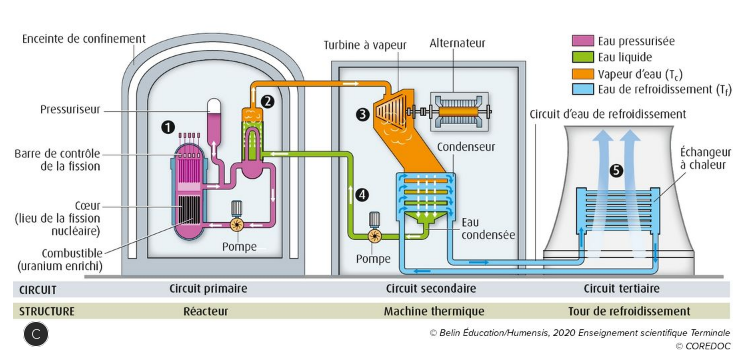
\includegraphics[width=0.9\linewidth]{figure/sch_centrale1}
	\caption[Schéma de principe d'une centrale nucléaire de type REP]{Schéma de principe d'une centrale nucléaire de type REP, d'après \cite{noauthor_manuel_nodate}}
	\label{fig:schcentrale1}
\end{figure} 
\subsection{Généralités sur la sûreté nucléaire}

Les questions relatives à la sûreté sont intrinsèquement liées à l'exploitation d'une centrale nucléaire tant les conséquences d'un éventuel accident peuvent être importantes. Ainsi dès le début des années 1970, le concept de défense en profondeur a été mis en place. ce dernier se matérialise par la mise en place de lignes de défense successives indépendantes. Les REP comptent trois barrières de confinement :
\begin{enumerate}
	\item La gaine combustible, constituée de zircaloy (alliage de zirconium) qui piège les produits radioactifs et notamment les gaz de fission dans les pastilles de combustibles ;
	\item La cuve et l'ensemble du circuit primaire ;
	\item Le bâtiment réacteur placé sous atmosphère dépressurisée, dernière barrière de confinement avant la contamination hors-site.
\end{enumerate}
Les variations par rapport au régime nominal sont classées selon l'échelle INES (International Nuclear Scale Event, figure \ref{fig:echelle-ines-article}), cette échelle permet de classifier les accidents selon les conséquences engendrées. Elle comporte huit échelons allant d'un simple écart (plusieurs centaines de cas par an en France) à l'accident majeur entraînant une contamination hors site. Les accidents correspondent aux paliers 4 à 7 et se différencient de l'incident du fait de la perte d'intégrité de la première barrière à la suite d'une fusion du combustible pour former un bain liquide issu du c\oe ur fondu : le corium.
\begin{figure}[H]
	\centering
	%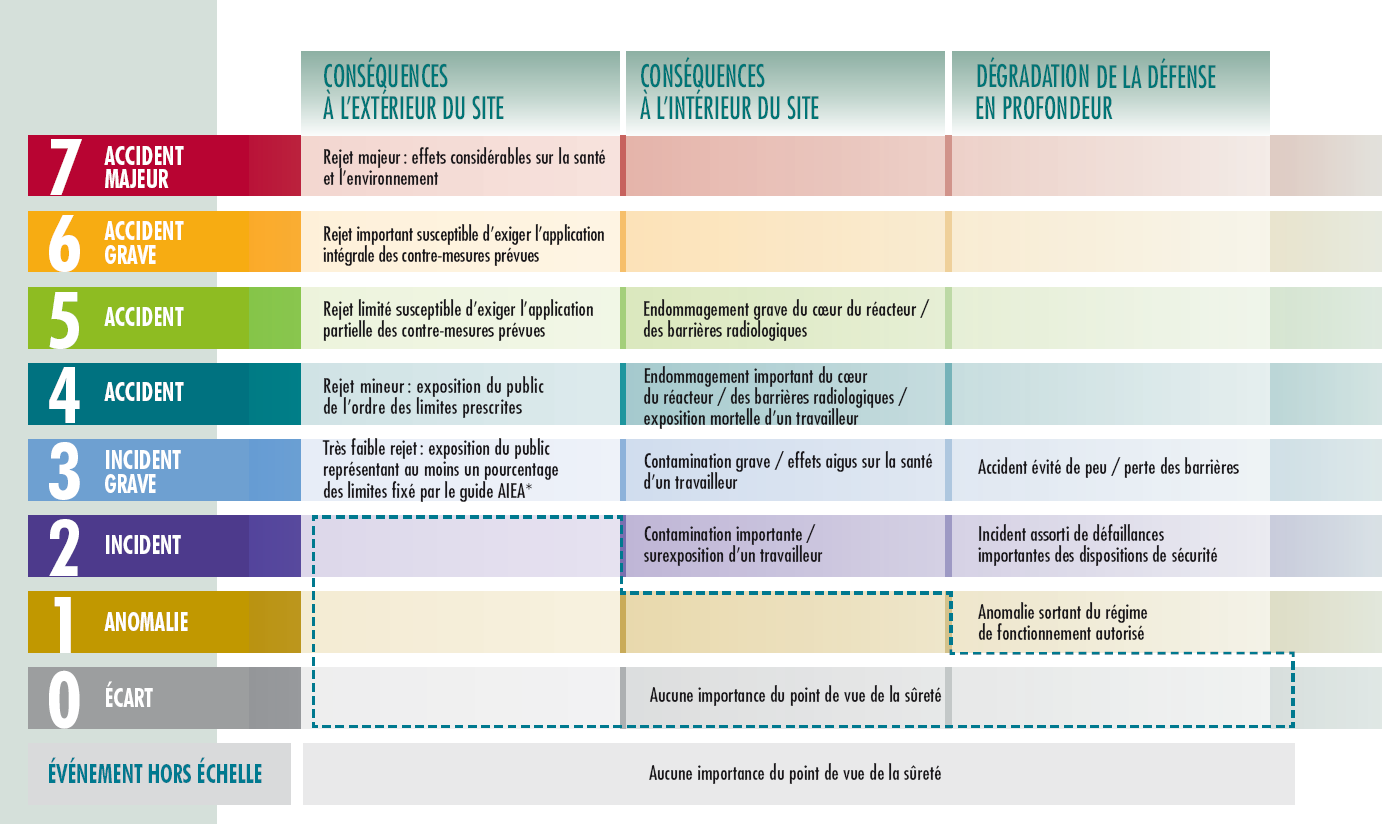
\includegraphics[width=1\linewidth]{figure/echelle-ines-article}
	\includegraphics[width=1\linewidth]{figure/RTN_ines}
	\caption[Echelle de classification des écarts au régime nominal INES]{Echelle de classification des écarts au régime nominal INES, d'après \cite{noauthor_risque_nodate}}
	\label{fig:echelle-ines-article}
\end{figure}
Les accidents possibles dans les REP sont séparés en deux grandes catégories : les accidents de criticité et les Accidents de Perte de Réfrigérant Primaire (APRP). Les accidents de criticité sont dus à une accélération brutale de la réaction en chaîne, le c\oe ur est alors en régime sur-critique ce qui entraîne une augmentation rapide de puissance thermique produite. L'accident de Tchernobyl en 1986, survenu sur un réacteur d'une technologie différente de celle des REP, est un exemple d'accident de criticité.\\ Les Accidents de Perte de Réfrigérant Primaire (APRP) résultent quant à eux d'une fuite dans le circuit primaire ou d'un arrêt de la circulation du fluide caloporteur privant le c\oe ur du refroidissement nécessaire à son fonctionnement, un cas d'accident de ce type est Fukushima Daiichi en 2011 où le tsunami a provoqué la perte d'alimentation électrique de la centrale, neutralisant ainsi l'ensemble des pompes. \\
Lors d'un accident de type APRP, l'élévation de la température dans le c\oe ur provoque l'oxydation fortement exothermique des gaines en zircaloy. La puissance produite par cette oxydation peut être, transitoirement,  supérieure à la puissance résiduelle liée à la désintégration naturelle des radioéléments. Sans refroidissement suffisant l'augmentation de température provoque la fusion du combustible, puis des éléments de contrôle du c\oe ur. Finalement le mélange issu de la fusion du combustible, des gaines partiellement oxydées et des structures internes du réacteur forme un bain liquide appelé corium. Le corium est un matériau fortement radioactif produisant sa propre chaleur, il est constitué d'uranium U, d'oxygène O, de zirconium Zr sous st\oe chiométrique ainsi que d'acier issu des structures.  L'objectif est alors de maîtriser la propagation de ce liquide, pour cela deux stratégies existent : la rétention en fond de cuve avec refroidissement externe, \textit{In-Vessel Retention, IVR} \cites{shi_cap1400_2019}{seiler_etudes_2010}. Pour limiter les conséquences d'un accident cette stratégie vise à maintenir le corium au fond de la cuve réacteur. Pour cela un refroidissement à l'extérieur de la cuve est mis en place. Cette stratégie est étudiée depuis les années 90 et mise en \oe uvre sur des réacteurs de faible puissance.
Une seconde stratégie, préférée pour les réacteurs de forte puissance, consiste à étaler le corium sur un radier en béton réfractaire \cite{bouteille_epr_2006}. Dans le cas de l'EPR, l'ablation du béton est limitée par un refroidissement passif mis en place sous le plancher, une fois le corium partiellement refroidi, celui-ci est finalement recouvert d'eau évitant ainsi une explosion de vapeur.\\
Dans la suite de ce rapport nous traiterons uniquement les cas d'accidents de type APRP et de rétention du corium en cuve \textit{IVR}.
\subsection{Stratégie de rétention du corium en fond de cuve (IVR)}
Le comportement du corium en fond de cuve est alors régi par deux principaux phénomènes \cite{shams_status_2020} : 
la thermochimie détermine le comportement des phases et leurs équilibres, en effet la présence d'une lacune de miscibilité pour la phase liquide du système \{U, O, Zr, Acier\} entraîne une stratification des phases liquides. En effet on distingue alors plusieurs phases dans le bain, une phase oxyde riche en oxygène et une ou plusieurs phases pauvre en oxygène notées métal. Le second phénomène concerne la thermohydraulique du bain, chaque phase est soumise à des mouvements de convection naturelle induite par les conditions aux limites associées (instabilité de Rayleigh-Bénard) et/ou le chauffage volumique associée à la puissance résiduelle.
%\subsubsection{Modélisation stationnaire}
Les premières études du comportement du bain de corium ont été réalisés pour des bains stationnaires. Il a été montré qu'en régime stationnaire la stratification comprend une phase oxyde et une phase métal \cite{theofanous_-vessel_1997}, cependant en fonction de l'accident la couche de métal peut être lourde (i.e plus que l'oxyde, on retrouve alors la configuration \ref{fig:confmetallourd}) ou légère (configuration \ref{fig:confmetalleger}). Les différents cas sont obtenus via des différences de conditions initiales (fraction massique d'acier, degré d'oxydation du zirconium, le rapport molaire entre l'uranium et le zirconium dans la phase oxyde et la température du bain). On distingue également, à certaines interfaces entre la cuve et le bain, la présence d'une croûte réfractaire issue de la solidification de la phase oxyde.
\begin{figure}[H]
	\begin{subfigure}[H]{0.47\textwidth}
		\begin{tikzpicture}[scale=0.60]
		%cuve
		%couche+croute
		\fill[red!50] (0.5,0) arc (180:360:4.5) -- cycle;
		%\fill[blue!10!gray!20] rectangle (9.5, 1);
		\fill[brown!80] (0.5,0) arc (180:360:4.5) -- (9.3,0) arc (360:180:4.3) -- cycle;
		\fill[brown!80] rectangle (9.5,0.1);
		\fill[blue!10!gray!20] (2.5,-3.5) ..controls +(0.9,-1.05)and+(-0.9,-1.05) .. (7.5,-3.5) -- cycle ;
	\fill[black!60] (0,1) -- (0,0) arc (180:360:5) -- (10,1) -- (9.5,1) -- (9.5,0) arc (360:180:4.5) -- (0.5,1) -- cycle;
\fill[brown!80] (0.5,0) arc (180:360:4.5) -- (9.3,0) arc (360:180:4.3) -- cycle;
%cuve
\draw (0,0) arc (180:360:5);
\draw (0.5,0) arc (180:360:4.5);
\draw (0,0) -- (0,1);
\draw (0.5,0) -- (0.5,1);
\draw (10,0) -- (10,1);
\draw (9.5,0) -- (9.5,1);
		
		%\draw (5,0.5) node[ scale=1.3]{couche d'acier};
		\draw (5,-2) node[ scale=1.5]{oxyde};
		\draw (5,-3.8) node[ scale=1.3]{métal lourd};
%		
%		\draw[->,>=latex, red, line width = 2mm] (1.3, 0.5) to (0.1, 0.5);
%		\draw[->,>=latex, red, line width = 2mm] (8.7, 0.5) to (9.9, 0.5);
		
		%FE
%		\draw[black, dashed, thick] (3.2,0.2) circle (0.8);
		%\draw[black, dashed, thick] (9.3,0.5) circle (0.8);
%		\draw[->,>=latex] (0.5, 0.8) to (4, 2);
%		\draw[->,>=latex] (9.3, 0.8) to (6, 2);
%		\draw (5,2.3) node[ scale=1.3]{Focusing Effect};
		
		%cuve
		\draw[->,>=latex] (-0.3, -3) to (1.2, -3);
		\draw (-0.3, -3) node[ scale=1, left]{cuve};
		
		%croute
		
		\draw[->,>=latex] (9, -5.2) to (7.8, -3.3);
		%\draw (1, -4.2) -- (-0.3, -4.2);
		\draw (11.5, -5.5) node[ scale=1, left]{croûte réfractaire};
		
		%echange
		%\draw[->,>=latex,line width = 0.8mm] (3.2, -0.6) to (3.2, -3.8);
		
		
%		\draw[->,>=latex,line width = 0.5mm] (2.8, 0.8) to (2.8, -1.2);
%		\draw (2.2,0.7) node[ scale=1]{(Fe)};
%		\draw[->,>=latex,line width = 0.5mm](3.5, -1.2) to (3.5, 0.8);
%		\draw (4.2,-1) node[ scale=1]{(U,Zr)};
		%\draw (2,0.5) node[ scale=1]{(Fe)};
		%\draw[->,>=latex,line width = 0.5mm](2.7, -1.2) to (2.7, 0.8);
		%\draw (3.4,-1) node[ scale=1]{(U,Zr)};
		%\draw[blue, very thick] (7.3, 0.1) -- (7.3, 1);
		%\draw[blue, thick] (7.2, 0.1) -- (7.4, 0.1);
		%\draw[blue, thick] (7.2, 1) -- (7.4, 1);
		%\draw (7.3, 0.5) node[ scale=1.3, right, blue]{$H$};
		\end{tikzpicture}
			\caption{Première configuration}
			\label{fig:confmetallourd}
	\end{subfigure}
	\hfil
	\begin{subfigure}[H]{0.47\textwidth}
	\begin{tikzpicture}[scale=0.60]
	%cuve
	%couche+croute
	\fill[red!50] (0.5,0) arc (180:360:4.5) -- cycle;
	%\fill[blue!10!gray!20] rectangle (9.5, 1);
	\fill[brown!80] rectangle (9.5,0.1);
	\fill[blue!10!gray!20] (0.5,0) rectangle (9.5, -1.2);
%	\fill[blue!10!gray!20] (2.5,-3.5) ..controls +(0.9,-1.05)and+(-0.9,-1.05) .. (7.5,-3.5) -- cycle ;
	\fill[black!60] (0,1) -- (0,0) arc (180:360:5) -- (10,1) -- (9.5,1) -- (9.5,0) arc (360:180:4.5) -- (0.5,1) -- cycle;
	\fill[brown!80] (0.5,0) arc (180:360:4.5) -- (9.3,0) arc (360:180:4.3) -- cycle;
	%cuve
	\draw (0,0) arc (180:360:5);
	\draw (0.5,0) arc (180:360:4.5);
	\draw (0,0) -- (0,1);
	\draw (0.5,0) -- (0.5,1);
	\draw (10,0) -- (10,1);
	\draw (9.5,0) -- (9.5,1);
	
	%\draw (5,0.5) node[ scale=1.3]{couche d'acier};
	\draw (5,-0.6) node[ scale=1.3]{métal léger};
	\draw (5,-2) node[ scale=1.5]{oxyde};
%	\draw (5,-3.8) node[ scale=1.3]{métal lourd};
	%		
	%		\draw[->,>=latex, red, line width = 2mm] (1.3, 0.5) to (0.1, 0.5);
	%		\draw[->,>=latex, red, line width = 2mm] (8.7, 0.5) to (9.9, 0.5);
	
	%FE
	%		\draw[black, dashed, thick] (3.2,0.2) circle (0.8);
	%\draw[black, dashed, thick] (9.3,0.5) circle (0.8);
	%		\draw[->,>=latex] (0.5, 0.8) to (4, 2);
	%		\draw[->,>=latex] (9.3, 0.8) to (6, 2);
	%		\draw (5,2.3) node[ scale=1.3]{Focusing Effect};
	
	%cuve
	\draw[->,>=latex] (-0.3, -3) to (1.2, -3);
	\draw (-0.3, -3) node[ scale=1, left]{cuve};
	
	%croute
	
		\draw[->,>=latex] (9, -5.2) to (7.8, -3.3);
%\draw (1, -4.2) -- (-0.3, -4.2);
\draw (11.5, -5.5) node[ scale=1, left]{croûte réfractaire};
	
	%echange
	%\draw[->,>=latex,line width = 0.8mm] (3.2, -0.6) to (3.2, -3.8);
	
	
	%		\draw[->,>=latex,line width = 0.5mm] (2.8, 0.8) to (2.8, -1.2);
	%		\draw (2.2,0.7) node[ scale=1]{(Fe)};
	%		\draw[->,>=latex,line width = 0.5mm](3.5, -1.2) to (3.5, 0.8);
	%		\draw (4.2,-1) node[ scale=1]{(U,Zr)};
	%\draw (2,0.5) node[ scale=1]{(Fe)};
	%\draw[->,>=latex,line width = 0.5mm](2.7, -1.2) to (2.7, 0.8);
	%\draw (3.4,-1) node[ scale=1]{(U,Zr)};
	%\draw[blue, very thick] (7.3, 0.1) -- (7.3, 1);
	%\draw[blue, thick] (7.2, 0.1) -- (7.4, 0.1);
	%\draw[blue, thick] (7.2, 1) -- (7.4, 1);
	%\draw (7.3, 0.5) node[ scale=1.3, right, blue]{$H$};
	\end{tikzpicture}
	\caption{Seconde configuration}
	\label{fig:confmetalleger}
\end{subfigure}
\caption{Présentation des différents régimes de stratification possibles}
\end{figure}
L'objectif de la rétention en cuve est alors de maintenir ce bain jusqu’à sa solidification, le refroidissement est assuré par de l'eau dans le puits de cuve et par rayonnement sur la face supérieur de la couche d'acier. Cependant la couche supérieure d'acier étant très conductrice et ayant un contact direct avec la cuve sur une surface très faible (la couche d'acier est haute de quelques dizaines de centimètres), la densité de flux transmise est très importante. Cet effet est appelé \textit{"focusing effect"} et représente la principale menace pour l'intégrité de la cuve.
%\subsubsection{Modélisation du régime transitoire}
Des études plus récentes ont montré que l'épaisseur de la couche d'acier pouvait être plus fine en régime transitoire qu'en régime stationnaire \cite{le_tellier_transient_2015}, diminuant ainsi la surface de contact et aggravant le \textit{"focusing effect"}, c'est pourquoi une modélisation en régime transitoire est désormais privilégiée. Lors du transitoire des phénomènes d'inversion de phase sont observés, une partie du métal de la phase légère s'alourdit sous l'effet d'un transfert de masse et des gouttes tombent, puis sous l'effet d'un même transfert de masse la phase lourde remonte. On observe alors trois couches : une couche d'oxyde, une de métal léger localisée au dessus de la couche d'oxyde et une couche de métal lourd en fond de cuve. Finalement, le schéma associé à l'étude du comportement d'un bain de corium en fond de cuve est présenté en figure \ref{fig:ivrschema}.
\begin{figure}[H]
	\centering
	\begin{tikzpicture}[scale=0.80]
	

	
	%couche+croute
	\fill[red!50] (0.5,0) arc (180:360:4.5) -- cycle;
	\fill[blue!10!gray!20] (0.5,0) rectangle (9.5, 1);
	
	\fill[brown!80](0.5,0) rectangle (9.5,0.1);
	%\fill[blue!10!gray!20] (0.5,0) rectangle (9.5, -1.2);
	\fill[blue!10!gray!20] (2.5,-3.5) ..controls +(0.9,-1.05)and+(-0.9,-1.05) .. (7.5,-3.5) -- cycle ;
	\fill[brown!80] (0.5,0) arc (180:360:4.5) -- (9.3,0) arc (360:180:4.3) -- cycle;
	%cuve
	\fill[black!60] (0,2) -- (0,0) arc (180:360:5) -- (10,2) -- (9.5,2) -- (9.5,0) arc (360:180:4.5) -- (0.5,2) -- cycle;
	%cuve
	\draw (0,0) arc (180:360:5);
	\draw (0.5,0) arc (180:360:4.5);
	\draw (0,0) -- (0,2);
	\draw (0.5,0) -- (0.5,2);
	\draw (10,0) -- (10,2);
	\draw (9.5,0) -- (9.5,2);
	
	\draw (5,0.5) node[ scale=1.3]{métal léger};
	\draw (5,-2.3) node[ scale=1.5]{oxyde};
	\draw (5,-3.8) node[ scale=1.3]{métal lourd};
	%\draw (6,-0.6) node[ scale=1.3]{métal léger};
	
	\draw[->,>=latex, red, line width = 2mm] (1.3, 0.5) to (0.1, 0.5);
	\draw[->,>=latex, red, line width = 2mm] (8.7, 0.5) to (9.9, 0.5);
	
	%FE
	%\draw[black, dashed, thick] (3.2,-1) circle (0.5);
	%\draw[black, dashed, thick] (9.3,0.5) circle (0.8);
	\draw[->,>=latex] (0.5, 0.8) to (4, 2);
	\draw[->,>=latex] (9.3, 0.8) to (6, 2);
	\draw (5,2.3) node[ scale=1.3]{Focusing Effect};
	
	%cuve
	\draw[->,>=latex] (-0.3, -3) to (1.2, -3);
	\draw (-0.3, -3) node[ scale=1, left]{cuve};
	
	%croute
	
	\draw[->,>=latex] (9, -4.2) to (7.8, -3.3);
	%\draw (1, -4.2) -- (-0.3, -4.2);
	\draw (11.5, -4.5) node[ scale=1, left]{croûte réfractaire};
	
	%echange
	\draw[->,>=latex,line width = 0.8mm] (3.2, 0) to (3.2, -3.8);
	
	
	\draw[->,>=latex,line width = 0.5mm] (2.8, -0) to (2.8, -1.3);
	\draw (2.2,-0.7) node[ scale=1]{(Fe)};
	\draw[->,>=latex,line width = 0.5mm](3.5, -1.3) to (3.5, -0);
	\draw (4.2,-1.5) node[ scale=1]{(U,Zr)};
	%\draw (2,0.5) node[ scale=1]{(Fe)};
	%\draw[->,>=latex,line width = 0.5mm](2.7, -1.2) to (2.7, 0.8);
	%\draw (3.4,-1) node[ scale=1]{(U,Zr)};
	%\draw[blue, very thick] (7.3, 0.1) -- (7.3, 1);
	%\draw[blue, thick] (7.2, 0.1) -- (7.4, 0.1);
	%\draw[blue, thick] (7.2, 1) -- (7.4, 1);
	%\draw (7.3, 0.5) node[ scale=1.3, right, blue]{$H$};
	\end{tikzpicture}
	\caption[]{Schéma du comportement du corium en fond de cuve en régime transitoire}
	\label{fig:ivrschema}
\end{figure}
La couche de métal lourd se forme à partir d'un transfert de masse à l'interface des phases oxyde et métal léger créant des gouttes de métal lourd se relocalisant en fond de cuve. Il existe peu de données expérimentales sur le comportement du corium en cuve du fait de la difficulté de réalisation expérimentale liée aux conditions de température supérieures à 2000K. MASCA RCW \cite{tsurikov_main_nodate} est une des rares expériences sur la stratification ayant mis en jeu une quantité suffisante de matière pour retranscrire la cinétique d'un accident. Cet essai utilise du corium prototypique (non radioactif) chauffé par induction. Lors de l'essai 45kg de corium ont été mis en contact avec 4kg d'acier, cette configuration permet d'obtenir un régime stationnaire caractérisé par la présence d'une phase métallique lourde (figure \ref{fig:confmetallourd}). L'essai a été arrêté avant que le système n'atteigne le régime stationnaire. Une photo de la découpe du lingot est présentée en figure \ref{fig:masca}. On y observe la présence de gouttes formées par des instabilités de Rayleigh-Taylor issus de la couche métallique légère. Aucune expérience similaire n'a permis d'observer le phénomène de remontée de la phase métallique lourde.

 \begin{figure}[H]
	\centering
	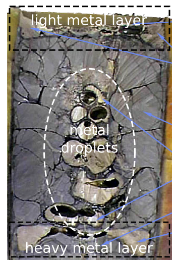
\includegraphics[width=0.3\linewidth]{figure/MASCA_RCW.png}
	\caption[Résultat MASCA-RCW 100]{Résultat MASCA-RCW, d'après \cite{tellier_interfaces_2019}}
	\label{fig:masca}
\end{figure}


\section{Objectif du stage}
Le LMAG s'intéresse à la modélisation du transfert de masse mis en jeu lors de transitoires de stratification pour mieux comprendre le comportement d'un bain de corium en fond de cuve. Pour permettre une meilleure compréhension des phénomènes le laboratoire développe deux types d'outils. Le premier est un modèle intégral implémenté dans la plateforme logicielle PROCOR \cite{le_tellier_phenomenological_2015}, développée au LMAG et utilisé par les industriels pour l’étude de la propagation du corium. Simultanément, des recherches sont également menées pour obtenir une modélisation à des échelles CFD (\textit{Computional Fluid Dynamic}) plus fines. Dans ce cadre une partie du laboratoire s'intéresse à la modélisation champ de phase pour considérer le transfert de masse aux interfaces lors de transitoires de stratification.\\ Les recherches ont commencé avec la thèse de C. Cardon \cite{cardon_modelisation_2016} sur la diffusion d'espèce dans un système multicomposant diphasique et le paramétrage associé en lien avec les bases thermodynamiques. Dans le cadre du contrat post-doctoral de R. Zanella l'étude de la faisabilité d'un modèle pseudo-binaire couplé à l'hydrodynamique a pu être menée. L'objectif était de reproduire qualitativement l'expérience MASCA-RCW \cites{zanella_two-_2020}{zanella_three-dimensional_2021} en utilisant un code pseudo-spectral. Finalement dans la thèse de M.A. Rasolofomanana \cite{rasolofomanana_modelisation_nodate} le couplage entre un système multicomposant multiphasique et l'hydrodynamique est réalisé au travers de l'implémentation de l'équation de Cahn-Hilliard généralisée dans TrioCFD  \cite{angeli_overview_2015} (code CFD Open-source CEA).\\
L'objectif général de ce stage est de tester ce modèle et son implémentation et de fournir des premiers éléments de validation. Pour ce faire, on s'intéressera en premier lieu au cas d'une goutte isolée dans une phase continue au travers d'une expérience de la littérature \cite{rao_influence_2015}. Cette expérience montre l’influence du transfert de masse sur la trajectoire d’une goutte multicomposant. En l'état du code, les simulations peuvent difficilement être quantitive, dans notre cas, on se limitera à une étude paramétrique et à des éléments de comparaison qualitatifs. Ensuite, de manière complémentaire, des simulations ont été réalisées afin d'évaluer la capacité de ce modèle à reproduire différents régimes de gouttes. Pour finir, en revenant vers l'objectif général associé à la simulation d'un bain de corium, une simulation de l'inversion de stratification d'un bain stratifié a été réalisée. \\
Le deuxième chapitre se concentre sur les notions théoriques liées à la méthode champ de phase et sur les choix de paramétrage du modèle. Le troisième chapitre présente les résultats pour une goutte isolée et non déformée soumise à du transfert de masse et la comparaison avec \cite{rao_influence_2015}. Dans le chapitre 4 certains régimes de déformation d'une goutte non soumise à du transfert de masse sont retrouvés. Le cinquième chapitre présente des simulations proche du cas d'intérêt du corium, avec des calculs d'instabilités de Rayleigh-Taylor entraînant l'inversion de stratification dans un bain. Finalement, au terme de ce rapport, une courte conclusion ainsi que des perspectives sont apportées.

% Le développement de ce type de code nécessite une compréhension des phénomènes à des échelles plus fine. Sans données expérimentales, la modélisation à l'échelle CFD (\textit{Computional Fluid Dynamic}).
%
%
%L'objectif du stage est de réaliser une validation qualitative d'un modèle CFD (\textit{Computional Fluid Dynamic}) implémenté dans TrioCFD, code Open-Source du CEA, par M.A Rasolofomanana lors de sa thèse \cite{rasolofomanana_modelisation_nodate}. Ce modèle est une généralisation de la méthode champ de phase pour un système multicomposant. Cette implémentation fait suite aux thèses de Clément Cardon \cite{cardon_modelisation_2016} et de Vaishnvi Tiwari \cite{tiwari_consistent_2019} sur la modélisation par la méthode de champ de phase pour un système multicomposant. L'expérience reproduite est présentée dans \cite{rao_influence_2015}, on y trouve une goutte qui sous l'effet d'un transfert de masse va subir une inversion de densité. Cette validation nécessite une paramétrisation cohérente du système pour obtenir des simulations consistante vis-a-vis d'un système binaire et du comportement thermodynamique. Le développement de ce type de code CFD a pour but de permettre la vérification et l'amélioration des lois de fermetures présente dans des codes intégraux, comme par exemple PROCOR développé au laboratoire.
\chapter{Éléments théoriques sur la méthode de champ de phase} \label{chap:2}
Ce deuxième chapitre résume l'ensemble des notions théoriques liées à la méthode champ de phase. Le couplage avec l'hydrodynamique est présenté puis une description analytique de l'énergie ainsi que les principales hypothèses du modèle sont introduites. 
\section{Présentation des principales méthodes de suivi et de capture d'interface}

Le traitement numérique efficace des interfaces représente un enjeu majeur de la simulation numérique tant les applications faisant intervenir des interfaces sont importantes. On différencie les méthodes de suivi d'interface des méthodes de capture d'interface. Les méthodes de suivi d'interface suivent des marqueurs placés sur l'interface au cours du temps, la position de l'interface est alors explicite. Les méthodes de capture d'interface quant à elle suivent implicitement l'interface au travers de l'évolution d'une fonction couleur. De nombreuses méthodes existent, on présente ici les principales :
\begin{itemize}
	\item[$\bullet$] \textit{\textbf{Volume of fluid (VOF) : }} Cette méthode utilise un maillage fixe découpé en cellule représentant des volumes. On associe alors à chacune de ces cellules une fraction volumique de fluide, cette proportion est alors résolue au cours du temps et la position de l'interface peut être reconstruite. Cette reconstruction a pour désavantage de ne fournir que peu d'informations viables sur l'interface. Cette méthode reste donc peu précise et est également difficile à mettre en \oe uvre en trois dimensions.
	\item[$\bullet$] \textit{\textbf{Méthode Level-Set (LS) : }}	Cette méthode repose sur la résolution implicite de l'interface au travers de la résolution d'une fonction auxiliaire dite fonction ligne de niveau, généralement la distance signée à l'interface. Cette fonction se doit d'admettre une valeur nulle à l'interface, ainsi au travers de la résolution d'une équation d'advection sur cette fonction ligne de niveau, l'interface est résolue. Cette méthode convient pour les problèmes à fort changement topologique mais présente le désavantage d'être non-conservative.
	\item[$\bullet$]\textit{\textbf{Arbitrary Lagrangian-Eulerian (ALE) : }} La méthode repose sur une double description lagrangienne (maillage mobile) et eulérienne (maillage fixe), à chaque itération temporelle, le maillage autour de l'interface est reconstruit pour s'adapter à la forme de l'interface, ainsi chaque maille contient uniquement un fluide. L'ensemble de ces propriétés rend la méthode très précise mais difficile à mettre en \oe uvre en trois dimensions.
	\item[$\bullet$]\textit{\textbf{Front-Tracking (FT) : }} La méthode utilise des marqueurs sans masse positionnés sur l'interface transportée suivant une description lagrangienne sur un maillage eulérien fixe. Ainsi les équations de Navier-Stokes sont résolues sur un maillage fixe tandis que l'équation régissant la position de l'interface est résolue sur un maillage mobile. La principale difficulté réside dans le choix des opérateur de communication entre les deux maillages. Cette méthode nécessite l'implémentation d'algorithme pour les cas de coalescence et rupture d'interface et possède comme désavantage de ne pas être conservative.
\end{itemize}








\section{Méthode champ de phase conservative}
\subsection{Présentation générale}
%Les méthodes de suivi ou de capture d'interface présentées précédemment décrivent toute l'interface comme une discontinuité, cependant il existe un second paradigme traitant l'interface comme une zone de transition continue, on parle alors d'interface diffuse. \\
Le traitement numérique de l'interface présente deux paradigmes : le premier traite l'interface comme une discontinuité. Le second modélise l'interface comme une zone de transition continue, on parle alors d'interface diffuse.
Dans ce second cas l'interface correspond donc à une zone d'épaisseur connue et maîtrisée où cohabitent les deux phases, les gradients à l'interface étant finis le traitement numérique est alors facilité. Ce concept d'interface diffuse date du XIX$^{\text{ème}}$siècle et est introduit par Van Der Walls \cite{rowlinson_translation_1979}.
\begin{figure}[H]
	\centering
	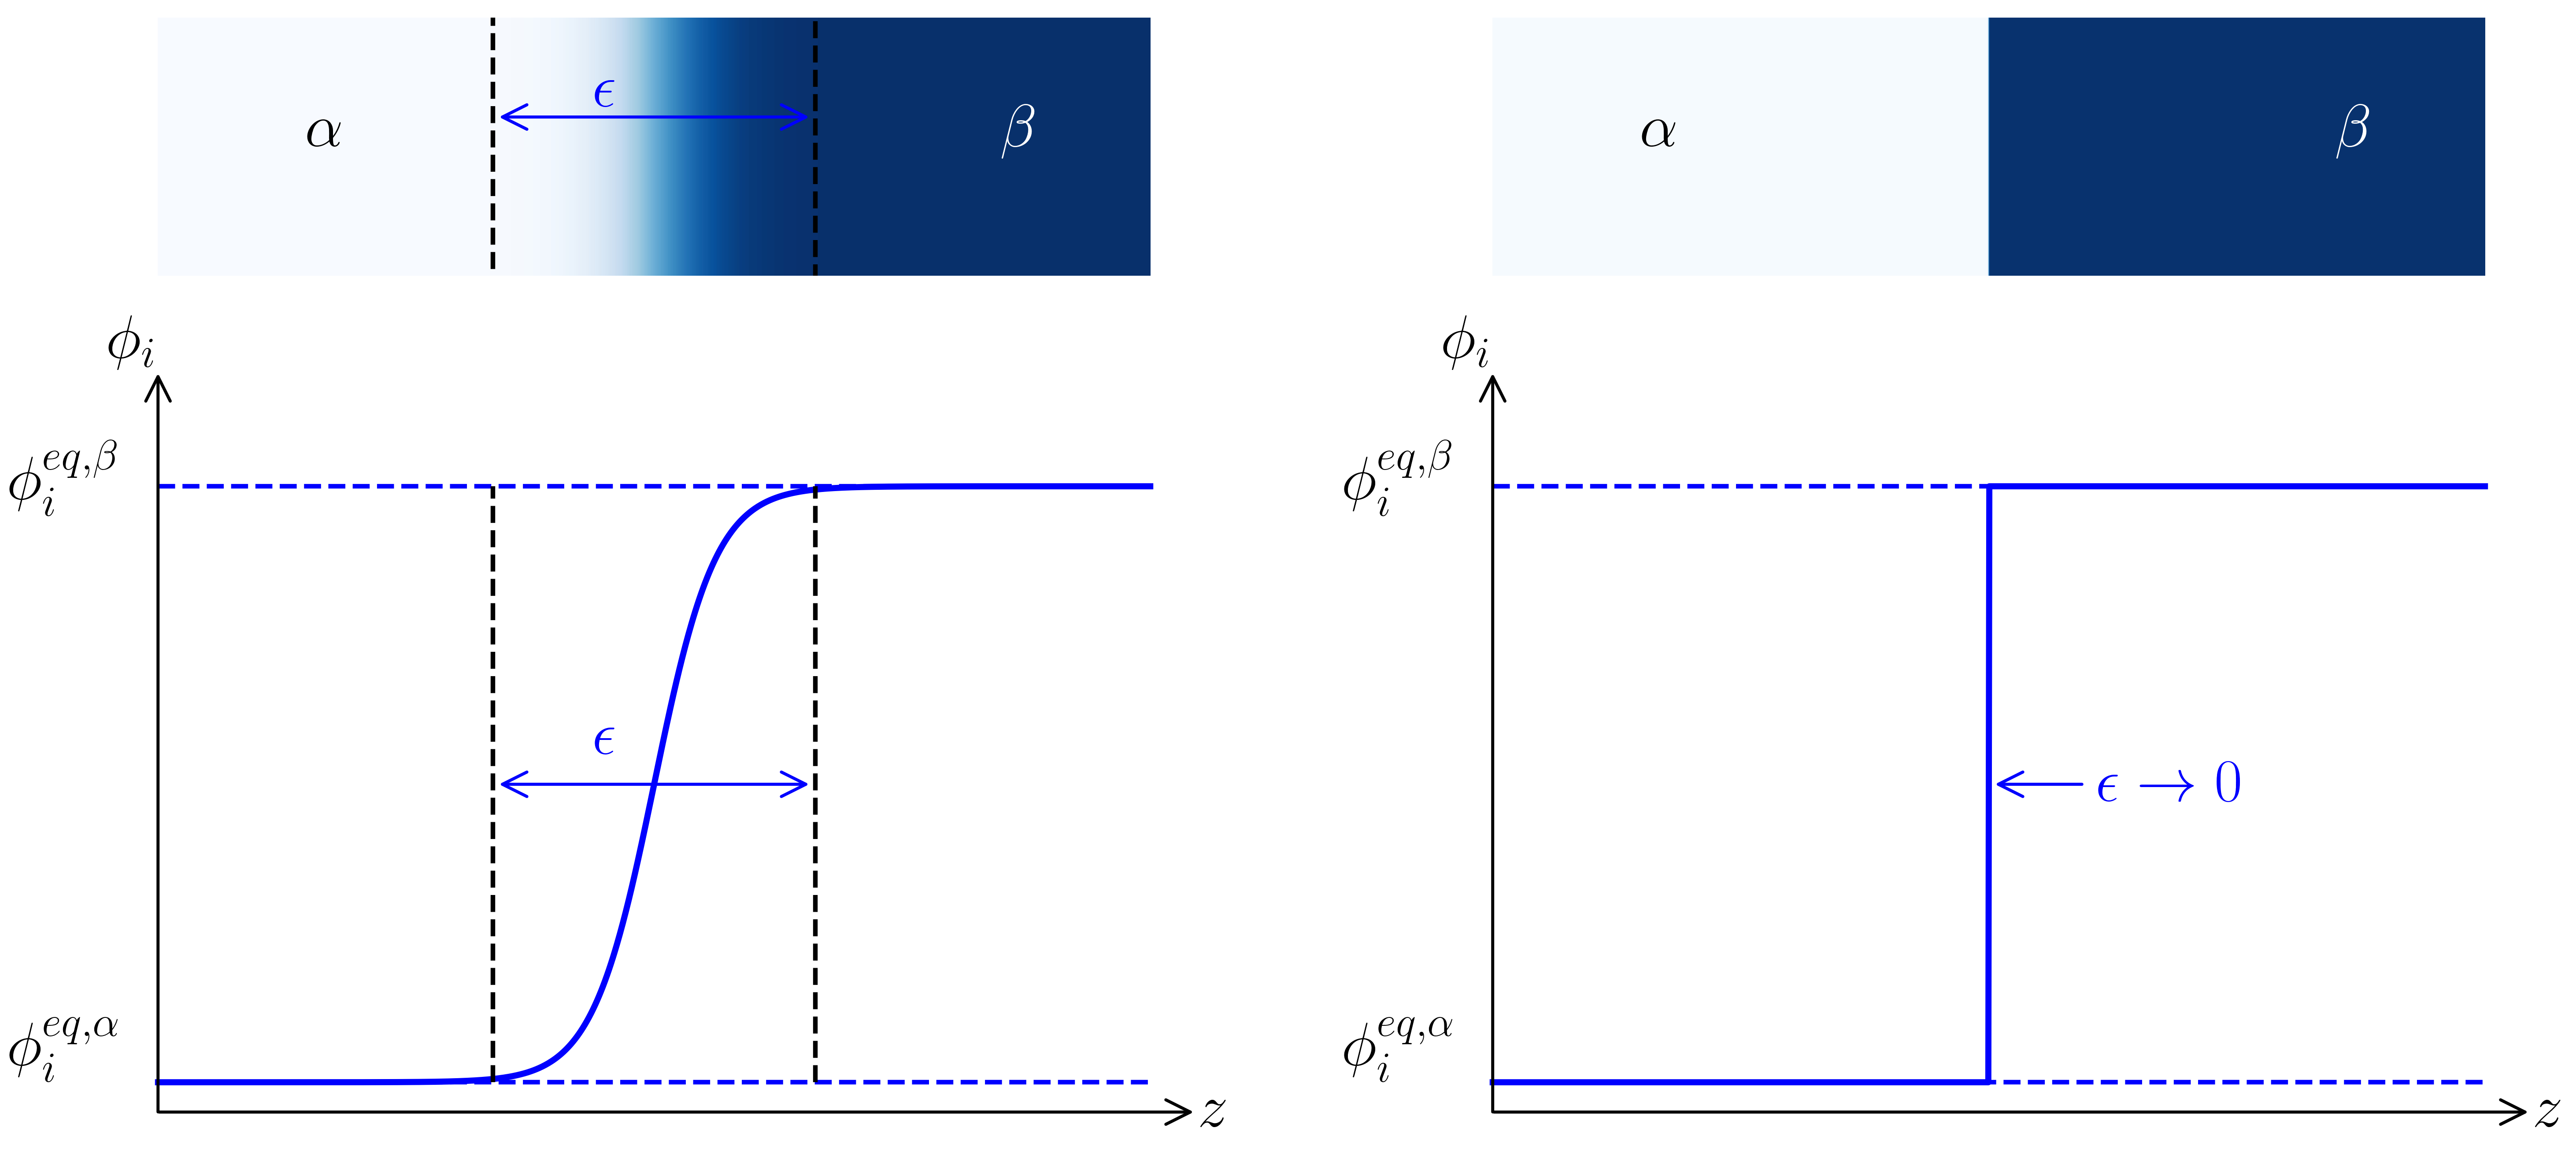
\includegraphics[width=0.5\linewidth]{figure/diffuse_interface}
	\caption{Comparaison entre une interface diffuse (à gauche) et une interface raide (à droite)}
	\label{fig:diffuseinterface}
\end{figure} 
 Le concept d'interface diffuse va gagner l'intérêt de la communauté scientifique avec le développement de la méthode champ de phase. En 1950, Ginzburg et Landau propose une description de l'énergie libre d'un système tenant compte des inhomogénéités spatiales (interfaces) en fonction d'un paramètre d'ordre \cite{landau_physique_1995}. En 1958, Cahn et Hilliard \cite{cahn_free_1958}  introduisent l'utilisation de cette description pour décrire l'évolution de la composition. Ces études sont la base de la méthode champ de phase. En effet la méthode champ de phase est basée sur la représentation d'un système au travers d'une fonctionnelle d'énergie libre, la description diffuse de l'interface et le suivi de paramètres d'ordre $\phi$. La méthode champ de phase est aujourd'hui utilisée dans de nombreux domaines, certains sont présentés en figure \ref{fig:champphase}.
\begin{figure}[H]
	\centering
	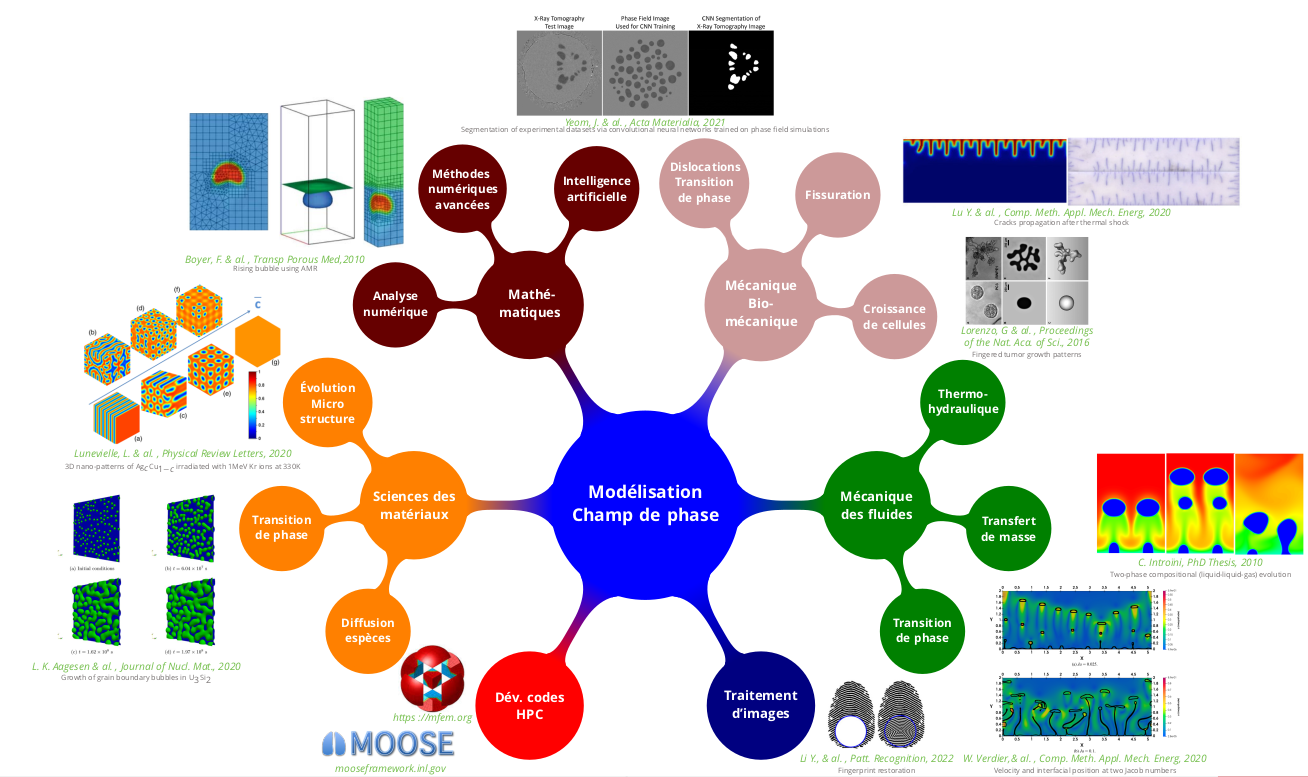
\includegraphics[width=0.9\linewidth]{figure/champ_phase}
	\caption[Domaine d'application de la méthode champ de phase]{Domaine d'application de la méthode champ de phase, tirée de \cite{introini_suivi_nodate}}
	\label{fig:champphase}
\end{figure} 
\subsection{Équation de Cahn-Hilliard généralisée}
Dans le cas n-composants on note $\{\phi_i\}_{i=1,..n}$ \footnote{Par soucis de simplification on pourra également utiliser la notation $\{\phi\}$} l'ensemble des paramètres d'ordre du système. Ces paramètres peuvent représenter la concentration, la fraction massique ou d'autres grandeurs.
Comme expliqué précédemment la méthode de champ de phase repose sur le suivi de ces variables. Ces paramètres d'ordre peut être conservés ou non, dans notre étude les paramètres d'ordres sont conservés. De plus on considère un système fermé, ainsi on obtient la contrainte :
\begin{equation}
\sum_{i=1}^n \phi_i =1 \Rightarrow \phi_n =1 - \sum_{i=1}^{n-1} \phi_i
\end{equation} 
Ainsi pour un mélange à $n$ composants, cette loi de fermeture permet de décrire l'ensemble du système en suivant l'évolution d'uniquement $n-1$ composants. Dans certains cas le système peut également être décrit avec des variables non conservées telles que des indicatrices de phases ou des grandeurs liées à des réactions chimiques. Le comportement de ces variables est alors régis par des équations de réaction-diffusion dites d'Allen-Cahn, non résolue dans cette étude. Dans le cadre de variables conservées les équations de Cahn-Hillard pour $n$ composants, avec $i\in \{1,..,n-1 \}$ s'écrivent sous la forme :
\begin{equation}
	\cfrac{\partial \phi_i}{\partial t} + \left(\mathbf{u} \cdot \nabla\right) \phi_i =  \nabla \cdot \left(\sum_{j=1}^{n-1}{\mathcal{M}_{ij}} \nabla\left( \frac{\delta \mathbb{F}}{\delta \phi_j}\right) \right) 
\end{equation}
avec : $\mathcal{M}_{ik}$ les coefficient de la mobilité (paramètre cinétique),  $\phi_i$ le paramètre d'ordre, $\mathbf{u}$ la vitesse et $\mathbb{F}$ une fonctionnelle de Ginzburg-Landeau généralisée \cite{cardon_modelisation_2016} définit tel que : 
 \begin{equation}
\mathbb{F}[\{\phi\}] = \int_{\mathcal{V}}\lambda\tilde{g}^{}(\{\phi\},\mathbf{x},t)+ \sum_{i=1}^{n-1}\sum_{j=1}^{n-1}\cfrac{1}{2}\kappa_{ij}\nabla \phi_i \cdot \nabla \phi_j dV
\end{equation}
Avec $\mathbf{x}$ le vecteur position et $V$ le volume.
Le premier terme représente la densité d'énergie liée aux valeurs locales de composition, traduisant l'équilibre des phases ainsi que leurs existences ou coexistence. Pour deux phases $\alpha$ et $\beta$, on rappelle les conditions données par l'équilibre thermodynamique \cite{kim_phase-field_1999} :
\begin{subequations}
	\label{eq:all}
	\begin{empheq}[left={\empheqlbrace\,}]{align}
		&\lambda\left.\frac{\partial \tilde{g}^{}}{\partial \phi_i}\right|_{\phi_i^{\alpha,eq}} = \lambda\left.\frac{\partial \tilde{g}^{}}{\partial \phi_i}\right|_{\phi_i^{\beta,eq}} = \tilde{\mu}_i^{eq} \\
& 		\lambda\tilde{g}^{\alpha,eq} - \sum_{i=1}^{n-1}\tilde{\mu}_i^{eq}\phi_i^{\alpha,eq} = 	\lambda\tilde{g}^{\beta,eq} - \sum_{i=1}^{n-1}\tilde{\mu}_i^{eq}\phi_i^{\beta,eq}
	\end{empheq}
\end{subequations}
$\tilde{\mu}_i^{eq}$ représente un potentiel de diffusion de l'élément $i$ à l'équilibre.\\
Le second terme représente la contribution des interfaces, le coefficient $\kappa_{ij}$, dit coefficient de gradient, tient compte du coût énergétique engendré par l'interface, par la suite ce paramètre pourra être relié à la tension de surface. \\
%Dans le cas binaire il est possible de décrire géométriquement l'ensemble des variables : 
%\begin{figure}[H]
%	\centering
%	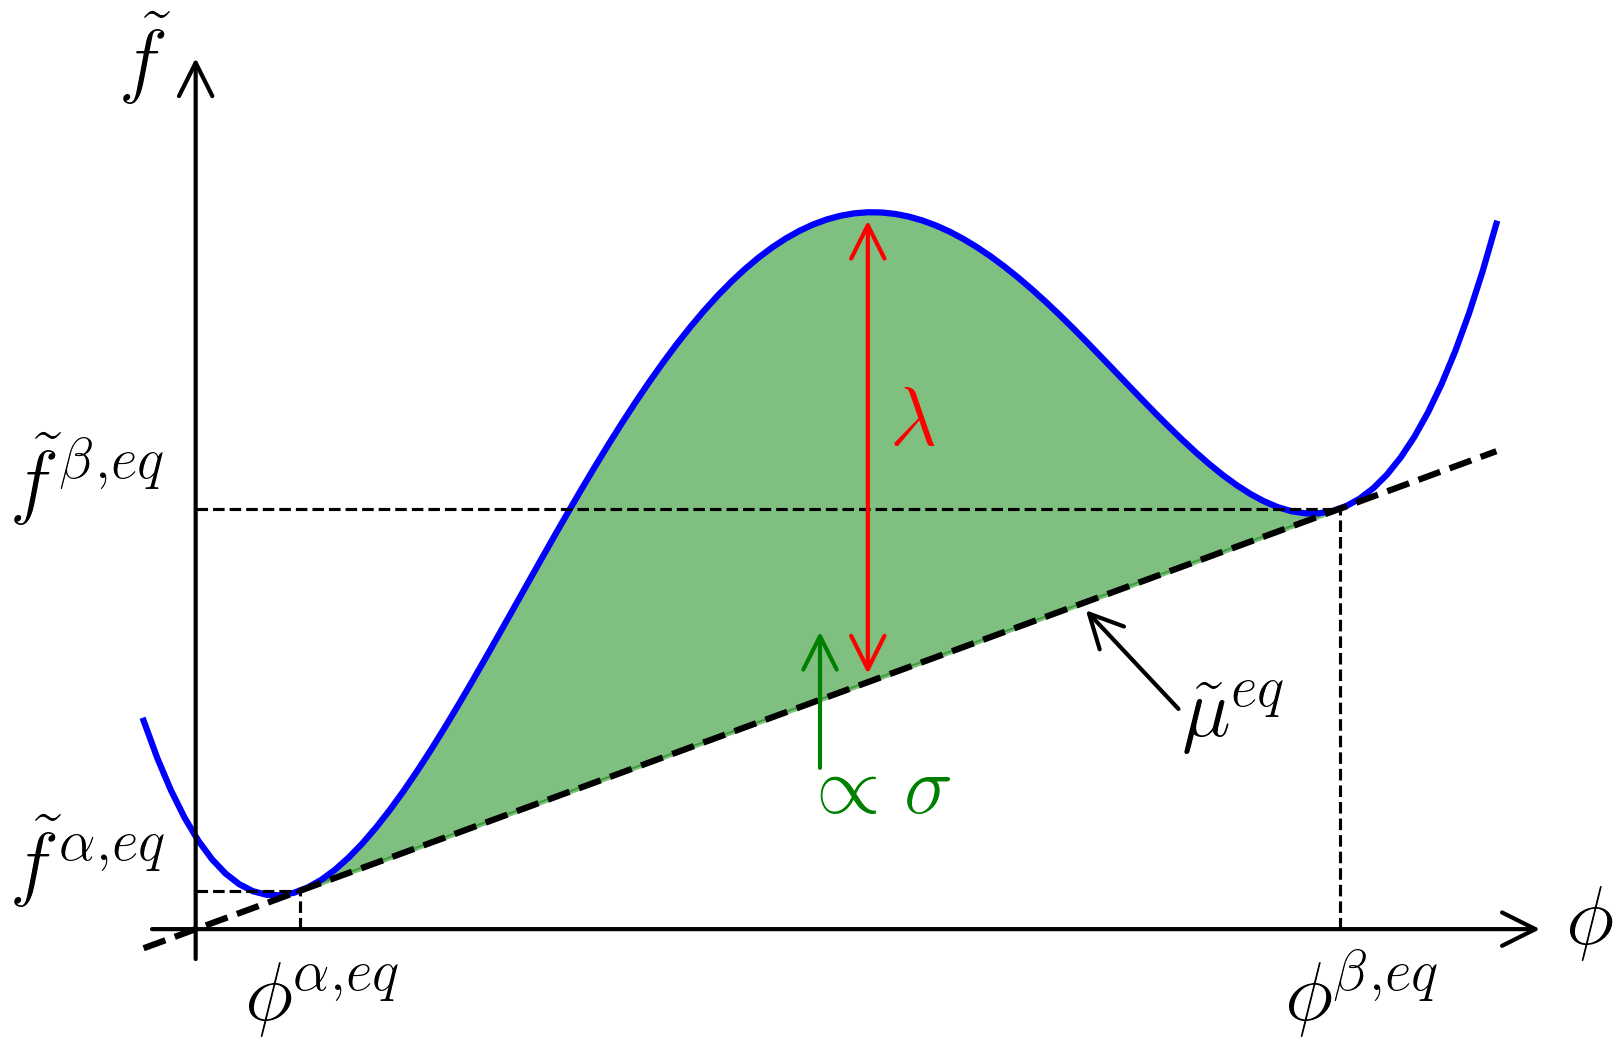
\includegraphics[width=0.45\linewidth]{figure/fig_NRJ}
%	\caption{Description de l'énergie libre pour un système binaire}
%	\label{fig:fignrj}
%\end{figure}
Finalement la dérivée variationnelle de cette fonctionnelle d'énergie libre peut être définie comme un potentiel de diffusion $\tilde{\mu}$: 
\begin{equation}\label{eq_potentiel}
	\frac{\delta \mathbb{F}}{\delta \phi_j} =\lambda \frac{\partial \tilde{g}}{\partial \phi_j} -\sum_{k=1}^{n-1} \kappa_{jk} \Delta \phi_k = \tilde{\mu}_j
\end{equation}
avec $\lambda$ un paramètre d'\textit{upscaling} numérique ajouté pour augmenter l'épaisseur de l'interface. Cet élargissement de l'interface permet d'utiliser des maillages réalistes compte tenu des capacités de calcul actuelles. \\
Le potentiel de diffusion peut être relié au potentiel chimique classique tel que :
%\begin{equation}
%	\tilde{\mu}_i = \frac{\lambda}{V_m}\left(\mu_i - \mu_n\right)
%\end{equation}
\begin{subequations}
	\begin{empheq}[left={\empheqlbrace\,}]{align}
	&\tilde{\mu}_i = \frac{\lambda}{V_m} \hat{\mu}_i \\
		& \hat{\mu}_i = \mu_i - \mu_n
	\end{empheq}
\end{subequations}
Avec $\tilde{\mu}_i$ (en J.m$^{-3}$) représente le potentiel de diffusion volumique de l'élément $i$, $\hat{\mu}_i$ (en J.mol$^{-1}$) le potentiel de diffusion molaire et $V_m$ le volume molaire supposé constant dans tout le système. \footnote{Dans le cadre de ce rapport on note $\tilde{.}$ les grandeurs volumiques}\\
%Le potentiel chimique étant classiquement définit tel que :
%\begin{equation}
%	\mu_i = \left.\frac{\partial G}{\partial n_i}\right|_{P,T,n_{j\neq i }} = \left.\frac{\partial F}{\partial n_i}\right|_{V,T,n_{j\neq i }}
%	  \textrm{                        où           } F = V_m f_0
%\end{equation}
%Avec $F$ (resp. $G$) l'énergie libre d'Helmotz (resp. Gibbs) (en J) et $n_i$ la quantité de matière de l'élément $i$ (en mol). Dans notre cas on se place dans une transformation isobare et isotherme, on privilégiera donc l'énergie de libre de Gibbs.
Dans le cas où $\doubleoverline{\kappa}$ = $\doubleoverline{0}$ on retrouve une équation d'advection-diffusion classique, dans le cas contraire on obtient une équation d'ordre 4. Pour un système binaire le gradient d'energie et le paramètre d'\textit{upscaling} peuvent être déterminés analytiquement. Dans le cas d'une modélisation à n-composants cette approche analytique ne fonctionne plus. Ainsi une des principales difficultés de la mise en place de la méthode champ de phase dans les cas n-aire est l'obtention de ces paramètres.
Dans la suite de ce travail nous utiliserons une proposition de paramétrage introduite par \cite{rasolofomanana_numerical_nodate} et présentée en annexe \ref{ann:parametrage}. Cette paramétrisation permet de déterminer les paramètres d'\textit{upscaling} $\lambda$ et le gradient d'énergie $\bm{\bar{\bar{\kappa}}}$ en fonction des paramètres physiques du système, la tension de surface $\sigma$ et l'épaisseur d'interface $\epsilon$. Ce paramétrage est construit de façon à être consistant vis-a-vis d'un système binaire.
\begin{subequations}
	\label{eq:all}
	\begin{empheq}[left={\empheqlbrace\,}]{align}
	&\bm{\bar{\bar{\kappa}}} = \frac{\sigma \epsilon}{\xi_1 \xi_2}\delta_{ij}
	\label{eq:1} \\
	&\lambda=\frac{\xi_2 \sigma}{2\epsilon\xi_1}
	\label{eq:2}
	\end{empheq}
\end{subequations}
avec $\xi_1 ,\xi_2$ deux constantes dépendantes de la description thermodynamique adoptée, $\delta_{ij}$ le symbole de Kronecker.
\subsection{Couplage avec les équations de Navier-Stokes incompressible}
Dans le cadre de cette étude, les équations de Cahn-Hilliard sont couplées aux équations de conservation de masse et de quantité de mouvement incompressible. Kim J. \cite{kim_phase-field_2012} présente un modèle \textit{one fluid} avec densité variable dans le terme de flottabilité. Les équations de Navier-Stokes s'écrivent sous la forme :
\begin{subequations}
	\label{eq:all}
	\begin{empheq}[left={\empheqlbrace\,}]{align}
	&\nabla \cdot \mathbf{u} = 0\\
	&\rho^* \left (\frac{\partial \mathbf{u}}{\partial t} + (\mathbf{u} \cdot {\nabla})\mathbf{u}\right) = -{\nabla} P +\eta \Delta \mathbf{u}+\sum_{i=1}^{n-1} \tilde{\mu}_i{\nabla} \phi_i + \rho\left(\{\phi_i\}\right) \mathbf{g}
	\end{empheq}
\end{subequations}
avec $\mathbf{u}$ la vitesse, $P$ la pression, $\mathbf{g} = \{ 0,0,-g\}^T $, $\eta$ la viscosité dynamique supposée constante, $\rho^*$ la masse volumique du solvant, $\rho\left(\{\phi_i\}\right)$ une loi de densité fonction du paramètre d'ordre. \\
L'hypothèse du volume molaire constant nous impose que la loi de densité soit une combinaison linéaire des masses volumiques des corps purs que l'on écrit sous la forme : 
\begin{equation}
	\rho\left(\{\phi_i\}\right) = \rho(\phi_n)\left(1+\sum_{i=1}^{n-1}\beta_i \phi_i\right)
\end{equation}
Les paramètres $\beta_i$ sont à déterminer en fonction du système étudié, $\rho(\phi_n)$ correspond à une masse volumique de référence, généralement celle du solvant.
\section{Paysage thermodynamique analytique}
\subsection{Introduction d'un pseudo-grand potentiel}
L'objectif présenté dans \cite{rasolofomanana_numerical_nodate} est d'obtenir une formulation analytique du terme homogène de la fonctionnelle de Ginzburg-Landau. Dans le cas binaire, cette contribution est de la forme d'un double puits, généralement un polynôme de degré 4.
L'objectif est de généraliser ce double puits pour un système n-aire, ainsi on introduit un pseudo grand potentiel correspondant à la hauteur énergétique nécessaire pour changer de minimum d'énergie \cite{cardon_modelisation_2016}.
\begin{equation}
\Omega^{\star} =\Omega - \Omega^{eq} =  {g} - \sum_i \hat{\mu}_i^{eq}\phi_i - \left(  {g}^{eq} -  \sum_i \hat{\mu}_i^{eq}\phi_i^{eq} \right) 
\end{equation}
avec ${g}^{}$ l'énergie libre de Gibbs (J.mol$^{-1}$)\footnote{En utilisant l'hypothèse du volume molaire constant il est possible d'écrire $\tilde{g} = {g}/{V_m}$}, utilisé comme grandeur d'intérêt ici puisque le système est supposé isotherme et isobare.
	\subsection{Application pour un cas diphasique ternaire}
Comme présenté au chapitre \ref{chap:1} le cas d'intérêt de l'étude est le corium. Ce système comprend deux phases à l'équilibre et donc deux points d'équilibre distinct.  Ainsi \cite{rasolofomanana_numerical_nodate} introduit une formulation sous la forme d'un double puits de la forme :
\begin{equation}\label{double_puit}
	\Omega^{\star}  = P^{dis} \times P^{cont}
\end{equation}
Où $P^{dis}, P^{cont}$ représentent deux paraboloïdes correspondant aux deux phases en présence à l'équilibre notées dispersée (ou drop) et continue. Dans le cas ternaire, en considérant les éléments d'intérêt notés miscible ($misc$)  et immiscible ($immi$)  : 
\begin{multline}
P^{k}=\left(\frac{\co{\theta^{k}}(\phi_{misc}-\phi_{misc}^{eq,k}) + \sinus{\theta^{k}}(\phi_{immi}-\phi_{immi}^{eq,k})}{a_{misc}^{k}}\right)^{2}+\\ \left(\frac{-\sinus{\theta^{k}}(\phi_{misc}-\phi_{misc}^{eq,k}) + \co{\theta^{k}}(\phi_{immi}-\phi_{immi}^{eq,k})}{a_{immi}^{k}}\right)^{2}
\label{eq:paraboloid_general_}
\end{multline}
Avec $k = \{disp,cont\}$ la phase (dispersée ou continue), $a_{misc}^k$ (resp. $a_{immi}^k$) le demi-petit (resp. demi-grand) puits, $\theta^k$ l'angle de rotation associé au puits de la phase $k$.\\
On trace alors en exemple le cas le plus simple de paysage :
\begin{figure}[H]
	\centering
	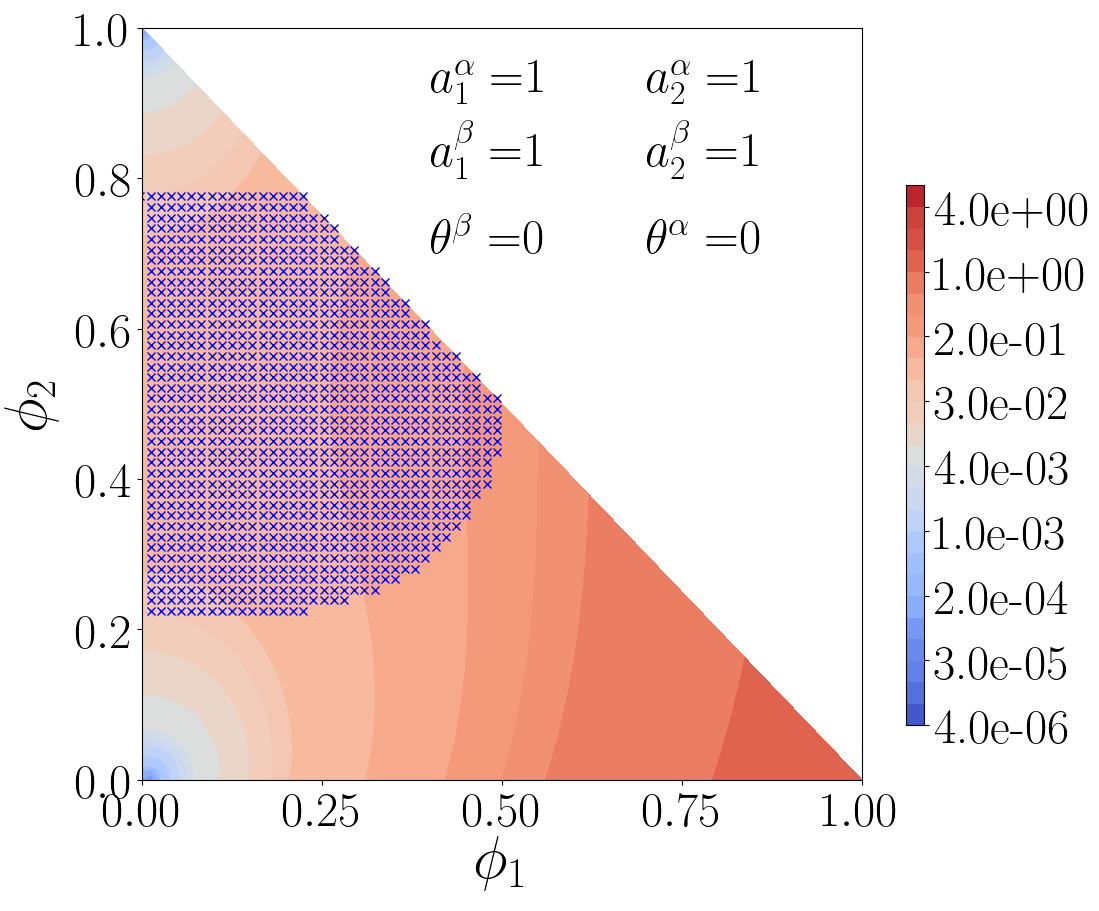
\includegraphics[width=0.6\linewidth]{figure/landscape}
	\caption{Exemple de paysage thermodynamique, la zone bleu représente la zone instable}
	\label{fig:landscape}
\end{figure}
%Les éléments de calculs pour la détermination de la zone instable sont présentés en annexe \ref{ann:stabphase}, cette zone correspond à des compositions pour lesquels le système subit une séparation de phase, ainsi il est primordiale que cette zone n'englobe pas les conditions initiales. Une représentation dans le plan est possible pour le cas ternaire, pour les cas comprenant un nombre plus important de paramètres d'ordre la visualisation semble plus complexe. Ainsi cette formulation possède l'avantage d'éviter un couplage entre le code CFD et un solveur d'équilibre thermodynamique (Open-Calphad par exemple) réduisant significativement le temps de développement. En effet pour les cas ou le paysage est connu il est alors possible de calibrer les paramètres des paraboloïdes pour obtenir une forme analytique proche du paysage réel. Dans le cas d'un paysage inconnu, par manque d'information thermodynamique, ce paysage permet d'avoir une description cohérente pour des simulations qualitatives.

La zone instable correspond à la zone où la séparation de phase a lieu, la détermination de cette zone est obtenue d'après \cite{aursand_spinodal_2017}. Une formulation analytique de cette forme permet d'éviter un couplage entre solveur d’équilibre thermodynamique (Open-Calphad par exemple) et le code CFD. Le temps de développement est alors fortement réduit. De plus, dans le cas d'un système sans données thermodynamiques, la formulation permet d'obtenir des simulations qualitatives. Dans le cas d'un système complètement décrit thermodynamiquement il suffit de trouver la formulation analytique qui convient (via un \textit{fit} par exemple). 


%On peut dès lors calculer le potentiel de diffusion homogène grâce à la formulation analytique (\ref{double_puit}) :
%\begin{align}
%	\tilde{\mu}_i & \nonumber= \frac{\partial}{\partial \phi_i}\left\lbrace 
%	\Omega^{\star} + \sum_j \tilde{\mu}_j^{eq}\phi_j + \left( {g}^{liq,eq} -  \sum_j \tilde{\mu}_j^{eq}\phi_j^{eq} \right)\right\rbrace \\
%	&\nonumber = \frac{\partial \Omega^{\star}}{\partial \phi_i} + \frac{\partial g^{liq,eq}}{\partial \phi_i} + \sum_j \frac{\partial \tilde{\mu}_j^{eq}\left(\phi_j - \phi_j^{eq}\right)}{\partial  \phi_i}\\
%	\tilde{\mu}_i &=	P^{dis}\frac{\partial P^{cont}}{\partial \phi_i} + P^{cont}\frac{\partial P^{dis}}{\partial \phi_i} + \tilde{\mu}_i^{eq}
%\end{align} 
%%\begin{align*}
%	%& \frac{\partial g^{liq,eq}}{\partial \phi_i} = 0 \\
%		%& \sum_j \frac{\partial \tilde{\mu}_j^{eq}\left(\phi_j - %\phi_j^{eq}\right)}{\partial  \phi_i} = \tilde{\mu}_i^{eq} %+\tilde{\mu}_{j\neq i}^{eq} \frac{\partial \phi_{j\neq i}}{\partial %\phi_i} = \tilde{\mu}_i^{eq}
%%\end{align*}
%L'objectif est alors de déterminer les paramètres des paraboloïdes pour obtenir des résultats consistants thermodynamiquement.



\chapter{Comparaison avec un cas de la littérature}
L'objectif de cette partie est de comparer les résultats obtenus par TrioCFD avec ceux présentés par Rao et al. \cite{rao_influence_2015}. Dans leur article Rao et al. présentent une expérience ainsi qu'un modèle CFD associé à l'experience permettant de modéliser le transfert de masse pour un cas ternaire.
\section{Présentation du cas de référence}
L'objectif de l'expérience est de visualiser la diffusion dans de l'eau de l'acétonitrile (miscible) contenue initialement dans une goutte composée également de chlorobenzène (non miscible). Ainsi à l'instant initial une goutte contenant un mélange d'acétonitrile et de chlorobenzène est formée, cette dernière étant plus légère que l'eau dans laquelle elle se trouve va commencer à monter, puis sous l'effet de la diffusion massique un changement de rapport de densité va subvenir et la goutte va redescendre.  
\begin{figure}[H]
	\centering
	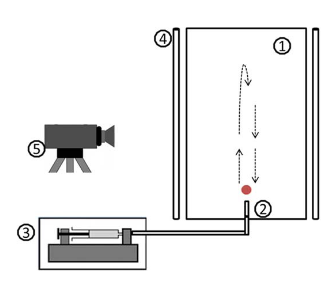
\includegraphics[width=0.3\linewidth]{figure/exp}
	\caption{Schéma de l'expérience, d'après \cite{rao_influence_2015}}
	\label{fig:exp}
\end{figure}
L'article présente également un modèle CFD, dans celui-ci le transfert de masse est calculé semi-empiriquement, à chaque itération la position de la goutte obtenue numériquement est comparée à la position obtenue expérimentalement, puis une régulation est mise en place pour déterminer un coefficient de transfert de masse via des corrélations pour faire diminuer cet écart, le ”modèle” alors obtenu n’est pas prédictible et une expérience physique est toujours nécessaire pour réaliser une simulation. L'algorithme est présenté en figure \ref{fig:algoRao}, 
\begin{figure}[H]
	\centering
	\begin{tikzpicture}[scale=0.75, transform shape]
	\node[draw,aspect=1.3, text centered,text width=3cm] (V) at (0,2.3) {Solution initiale };
	\node[draw,aspect=1.3, text centered,text width=2cm] (T) at (0,1.3) {$n=n+1$ };
	\node[draw,rectangle, text centered,minimum width=2cm,minimum height=1cm] (A)at(0,0){Estimation du transfert de masse à partir de corrélations};
	\node[draw,text centered,minimum width=2cm,minimum height=1cm] (B) at (0,-1.5) {Résolution des équations de Navier-Stokes};
	\node[draw,text centered,text width=10cm,minimum height=1cm] (C) at (0,-3) {Comparaison entre l'altitude de la goutte obtenue par CFD avec l'expérience, res = $f(z_{\text{CFD}},z_{\text{exp}})$};
	\node[draw,rectangle,diamond, aspect=1.3, text centered,text width=1.5cm] (D) at (0,-5) {res $<\varepsilon$ ? };
	
	\node[draw,rectangle,diamond, aspect=1.3, text centered,text width=1.5cm] (E) at (0,-7.3
	) { $t^{f}<t^{n}$ ? };
	\node[draw,aspect=1.3, text centered,text width=1.5cm] (W) at (0,-9) {Fin};
	%\node[draw,text centered,text width=2cm,minimum height=1cm] (E) at (0,-6.8) { $t=t^{n+1}$};
	%\node[draw,text centered,text width=7cm,minimum height=1cm] (Z) at (0,-6.2) { dsq}
	
	\node[draw,rectangle,diamond, aspect=1.3, text centered,text width=1cm,color=white] (H)at(-5,-5.9){ };
	\node[text centered,text width=1cm,color=black] (K1)at(0.5,-5.9){oui};
	\node[text centered,text width=1cm,color=black] (K2)at(-1.5,-4.8){non};
	\node[text centered,text width=1cm,color=black] (K3)at(0.5,-8.3){oui};
	\node[text centered,text width=1cm,color=black] (K4)at(-1.5,-7){non};
	%\node[draw,rectangle, text centered,diamond, aspect=1.3, text centered,text width=1cm] (I)at(6,-6){i=1 to n-1};
	\draw[->] (T.south) -- (A.north);
	\draw[->] (A.south) -- (B.north);
	\draw[->] (B.south) -- (C.north);
	\draw[->] (C.south) -- (D.north);
	\draw[->] (D.south) -- (E.north);
	\draw[->] (V.south) -- (T.north);
	\draw[->] (E.south) -- (W.north);
	\draw[->] (-7,1.3) -- (T.west);
	
	
	
	\draw (D.west)-- (-6,-5);
	\draw (-6,-5)-- (-6.,0);
	%	\draw (F.west)-- (-6.,0);
	\draw[->] (-6.,0) -- (A.west);
	\draw[-] (E.west) -- (-7,-7.3);
	\draw[-] (-7,-7.3) -- (-7,1.3);
	%\draw (G.east)-| (I.south);
	%\draw[->] (I.north)|- (A.east);
	\end{tikzpicture}
	\caption{Algorithme de résolution développé par Rao et al.\cite{rao_influence_2015}}
	\label{fig:algoRao}
\end{figure}
\section{Simulation réalisées}
\subsection{Choix du paysage thermodynamique}
L'objectif est alors d'utiliser un paysage de ce type pour résoudre un problème donné, pour cela quelques règles sont à garder en tête pour le choix d'un paysage thermodynamique. Dans un premier temps il est essentiel que les conditions initiales ne soient pas incluse dans la lacune de miscibilité, ce qui entraînerait une séparation de phase immédiate, un exemple de paysage de ce type est donnée en figure \ref{fig:landscapebase} et les résultats sont présentés par la figure \ref{land_base_sep}, on y observe une séparation de phase dès les premiers instants du calcul .
 \begin{figure}[H]
 	\centering
 	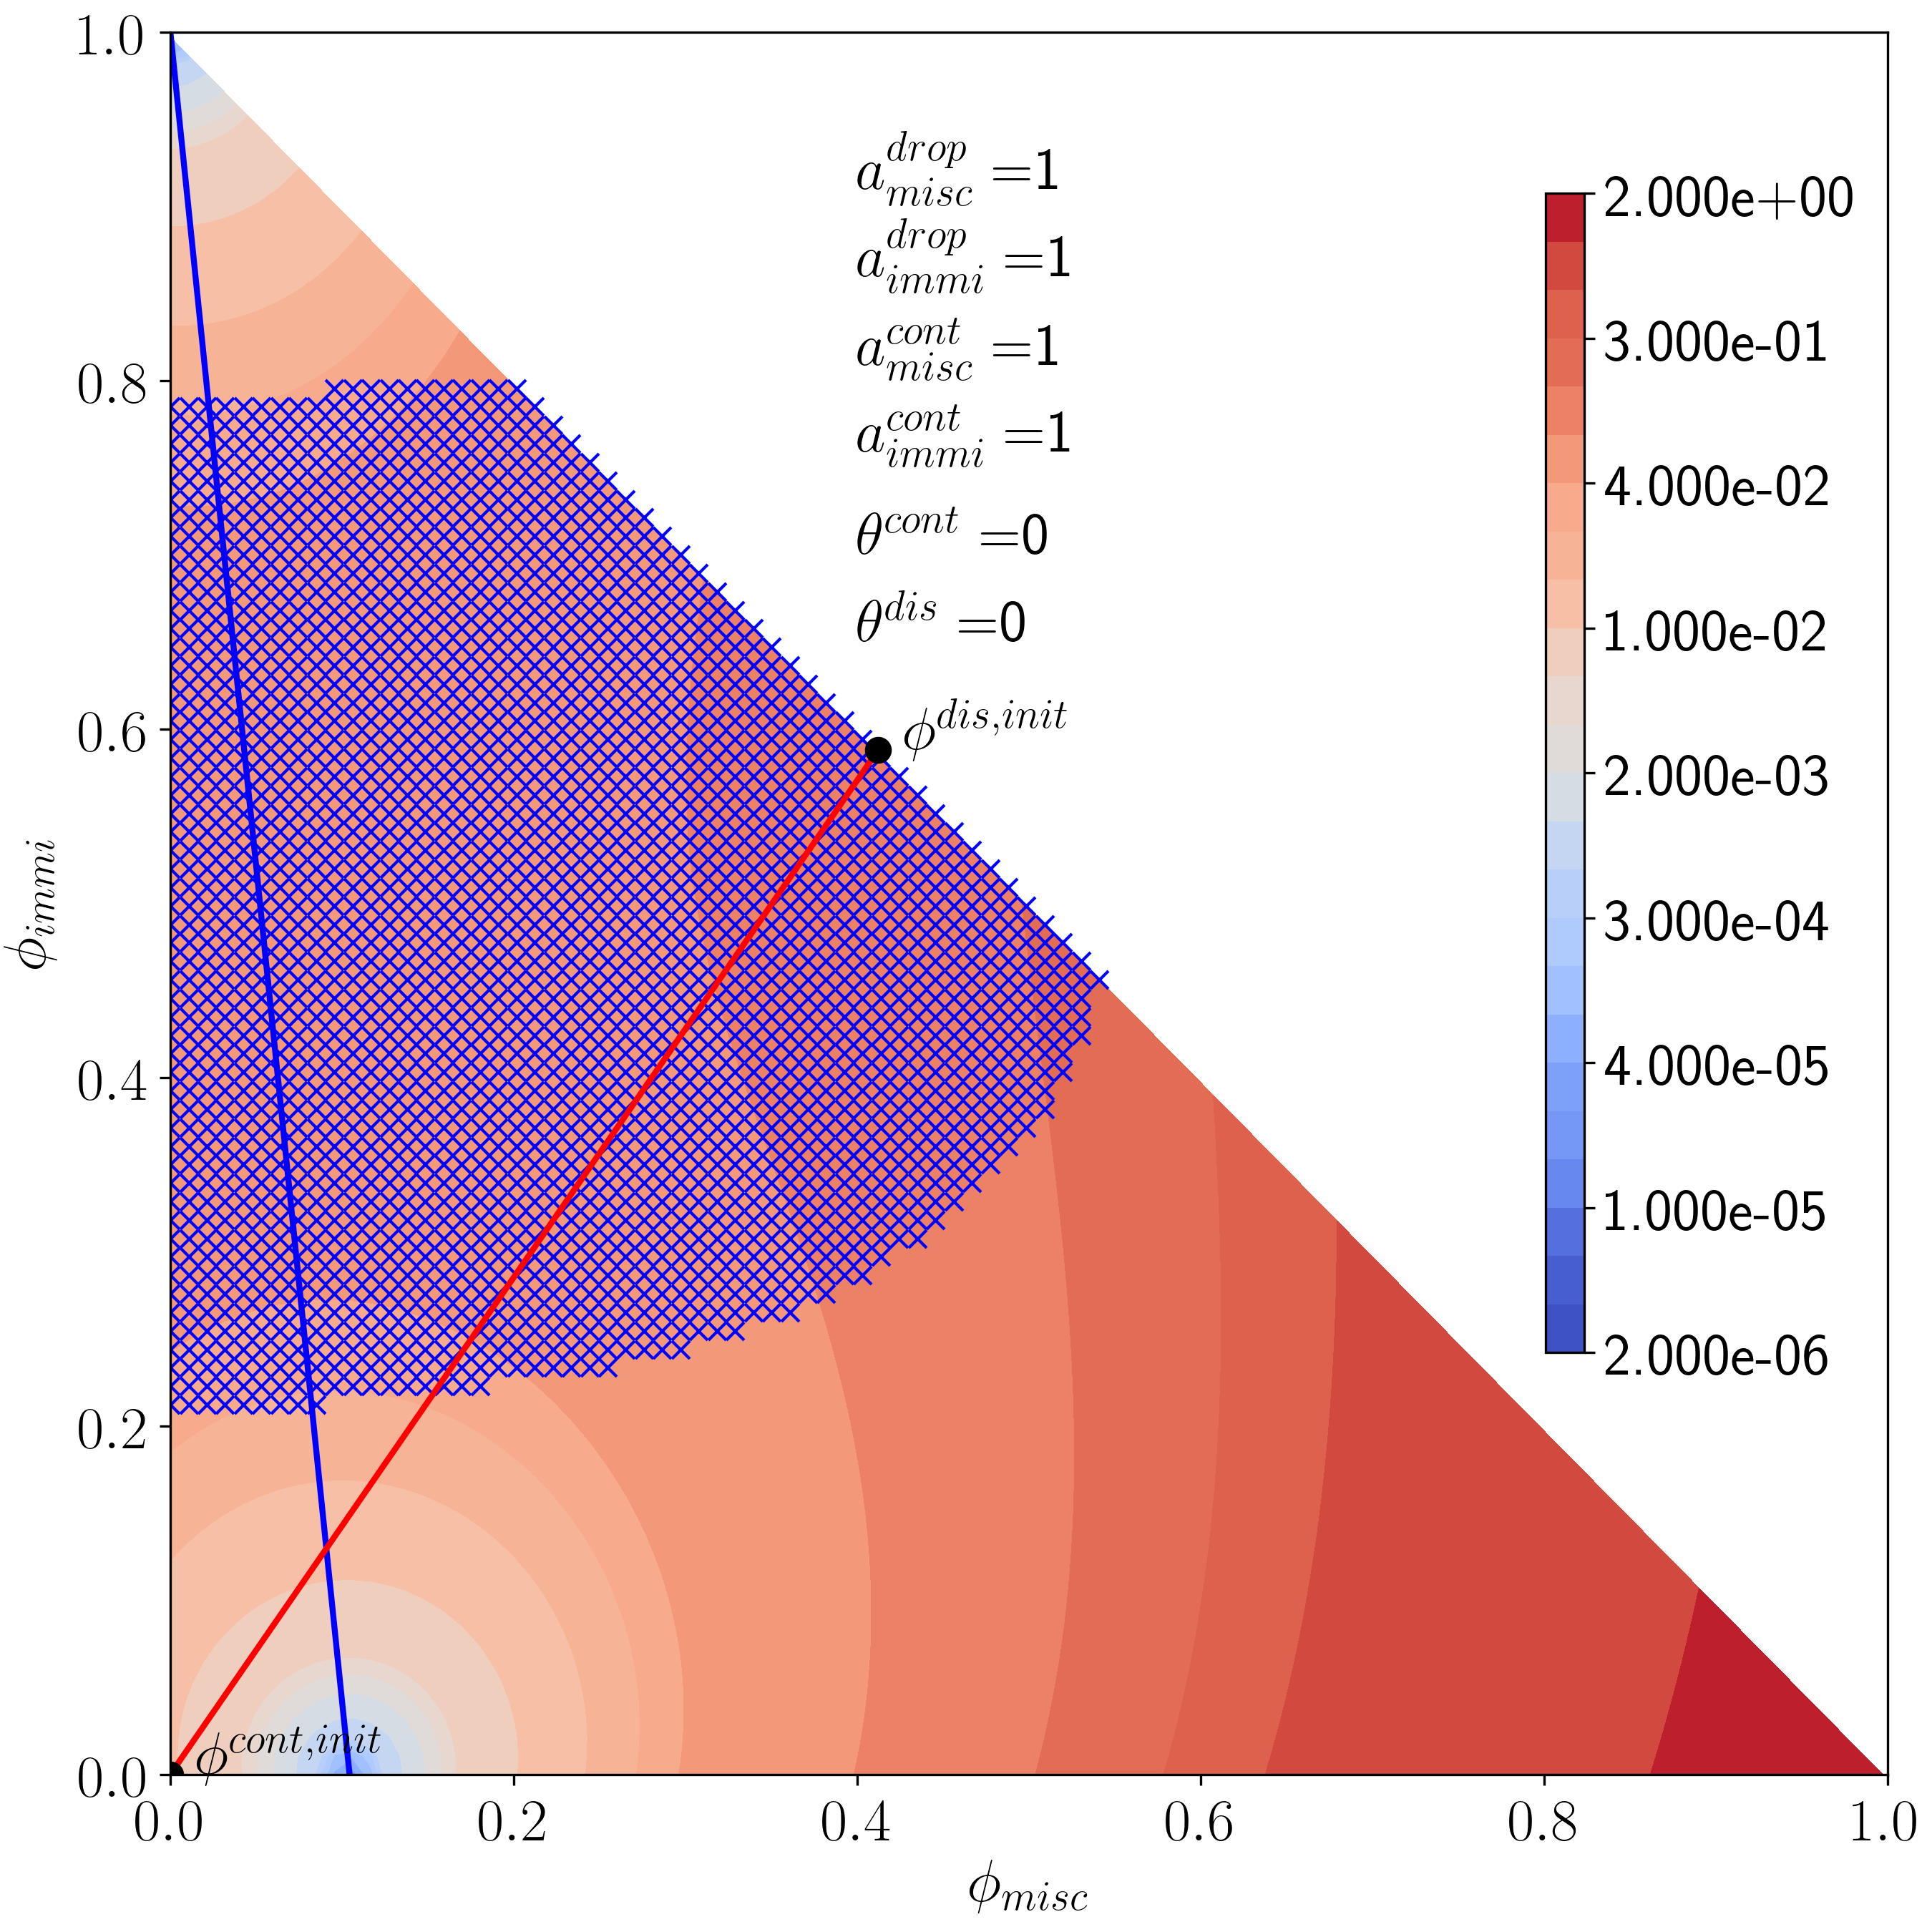
\includegraphics[width=0.4\linewidth]{figure/landscape_base.png}
 	\caption[Paysage thermodynamique]{Paysage thermodynamique, la droite bleu relie les deux  concentrations d'équilibre, la droite rouge relie les deux concentrations initiales}
 	\label{fig:landscapebase}
 \end{figure}
\vspace{-0.5cm}
 \begin{figure}[H]
 	\centering
 	\begin{subfigure}[H]{0.32\textwidth}
 		\centering
 		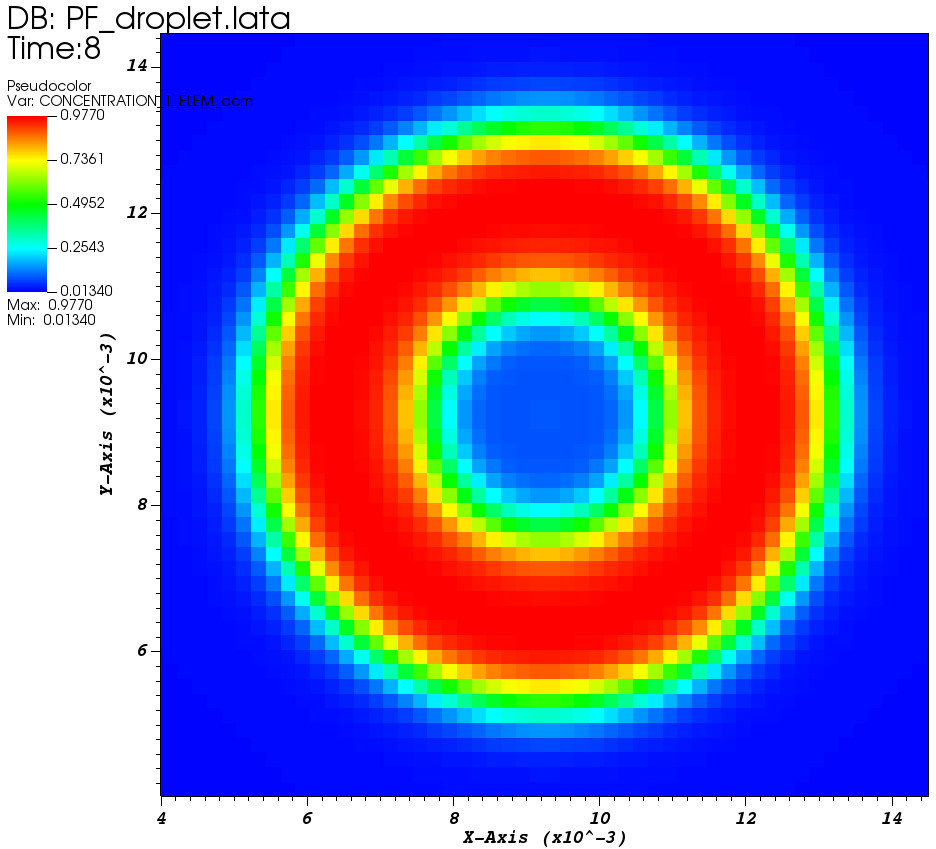
\includegraphics[width=\textwidth]{figure/paysage_base/visit0000.png}
 		\caption{Concentration immiscible}
 		\label{fig:y equals x}
 	\end{subfigure}
 	\begin{subfigure}[H]{0.32\textwidth}
 		\centering
 		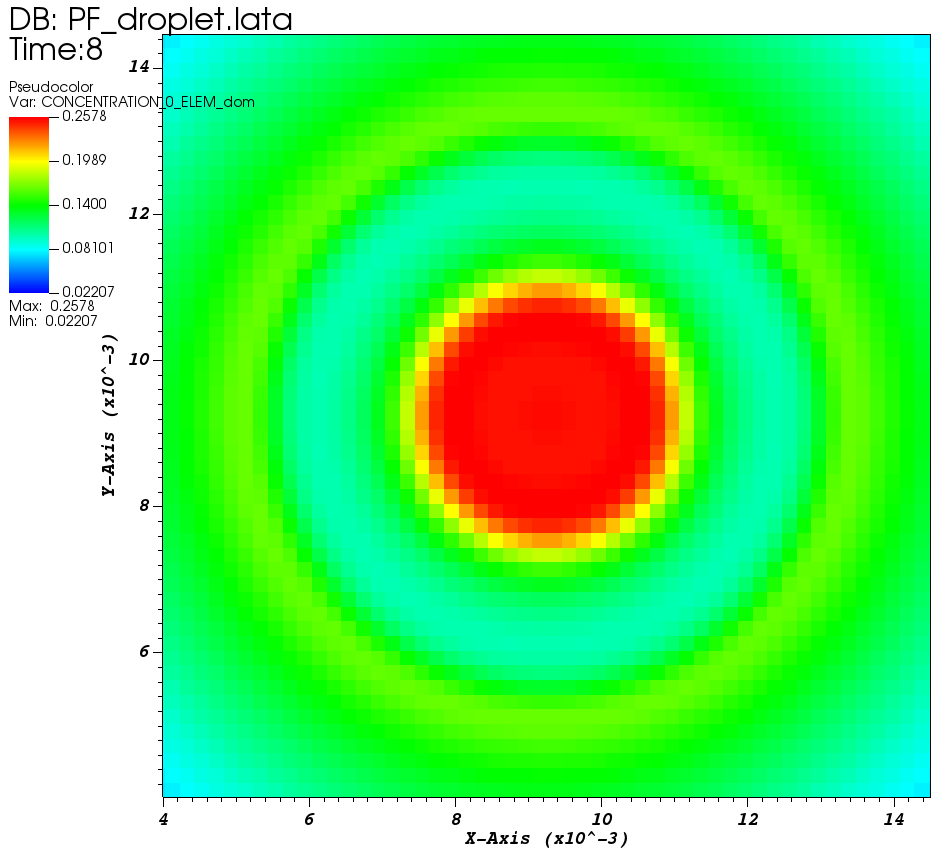
\includegraphics[width=\textwidth]{figure/paysage_base/visit0001.png}
 		\caption{Concentration miscible}
 		\label{fig:y equals x}
 	\end{subfigure}
 	\begin{subfigure}[H]{0.32\textwidth}
 		\centering
 		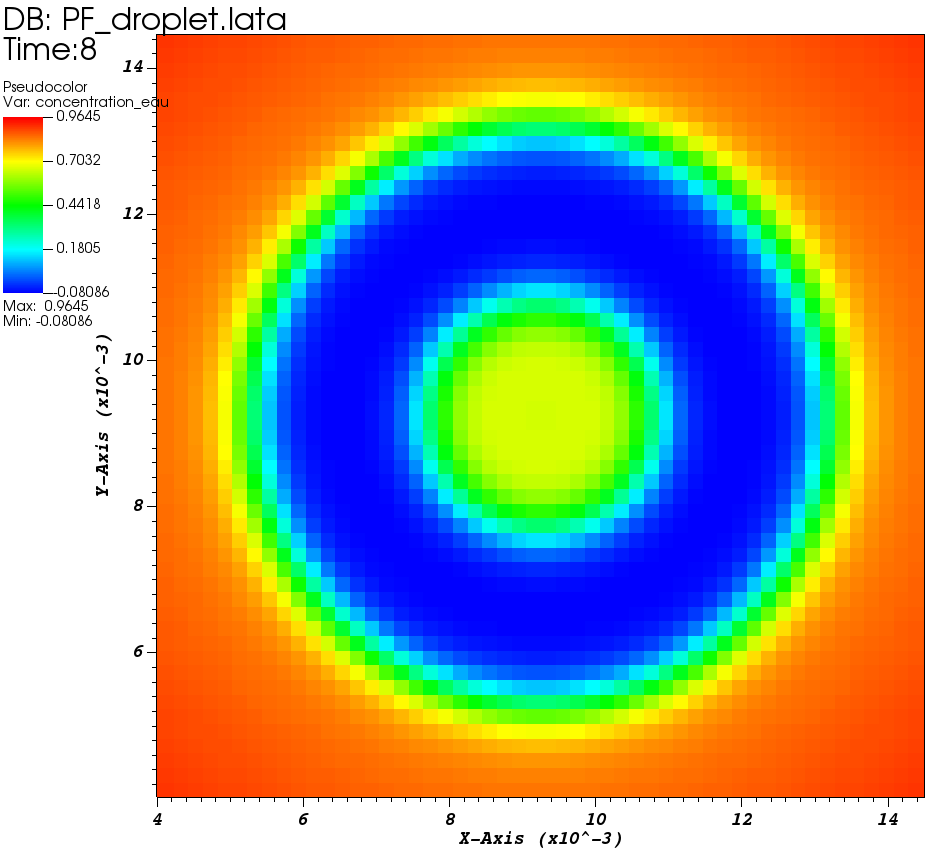
\includegraphics[width=\textwidth]{figure/paysage_base/visit0002.png}
 		\caption{Concentration eau}
 		\label{fig:y equals x}
 	\end{subfigure}
 	\caption{Séparation de phase dans la goutte}
 	\label{land_base_sep}
 \end{figure} \vspace{-0.5cm}
Sur la figure \ref{land_base_sep} on observe la présence de deux phases à l'intérieur de la goutte, une première uniquement composée de l'élément immiscible et la seconde composée d'eau et de l'élément miscible. On présente un deuxième paysage en figure \ref{fig:paysage2}
Comme expliqué précédemment ce paysage représente l'énergie libre volumique liée à l'équilibre des phases, ainsi on cherche à ce que les conditions initiales (ici aux extrémités de la droite rouge) soit hors de la zone instable et que la composition d'équilibre globale (placé a l'intersection des droites bleu et rouge) soit placée dans la lacune de miscibilité. Ainsi ce paysage semble correspondre parfaitement à ces deux critères. On souhaite également limiter l'entrée d'eau dans la goutte en régime transitoire, cette condition ce traduit par égalité entre la somme des deux compositions et l'unité. Hors ici le gradient d'énergie favorise un "chemin" différent. Pour vérifier cette présence d'eau, on considère alors un calcul statique (sans résolution des équations de Navier-Stokes) et on trace les concentrations à différents instants. On observe dès lors une importante intrusion d'eau dans la goutte dès les premiers instants, puis une séparation de phase est observable à l'intérieur de la goutte, phénomène que l'on souhaite absolument éviter.
 \begin{figure}[H]
 	\centering
 	\begin{subfigure}[H]{0.45\textwidth}
 		\centering
 		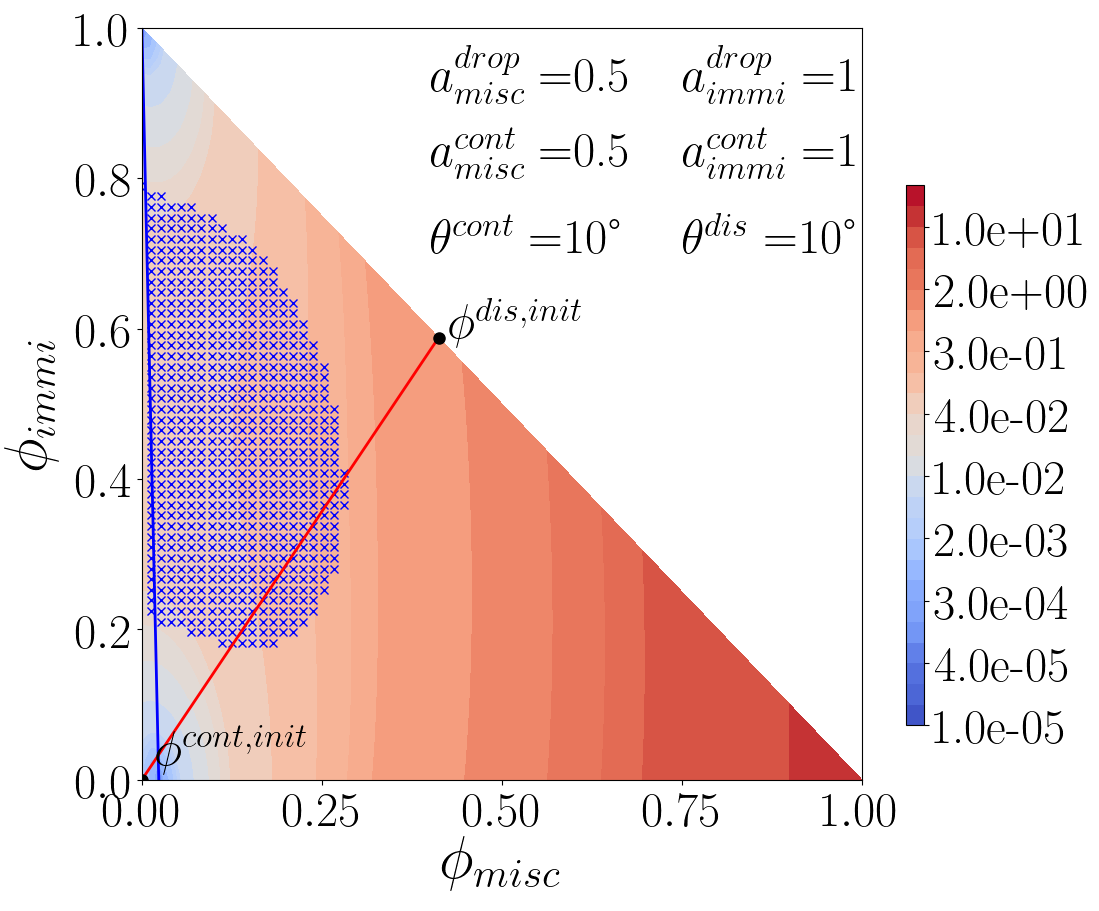
\includegraphics[width=\textwidth]{figure/paysage_neqlocal}
 		\caption{Paysage thermodynamique complet}
 		\label{fig:y equals x}
 	\end{subfigure}
 	\hfill
 	\begin{subfigure}[H]{0.45\textwidth}
 		\centering
 		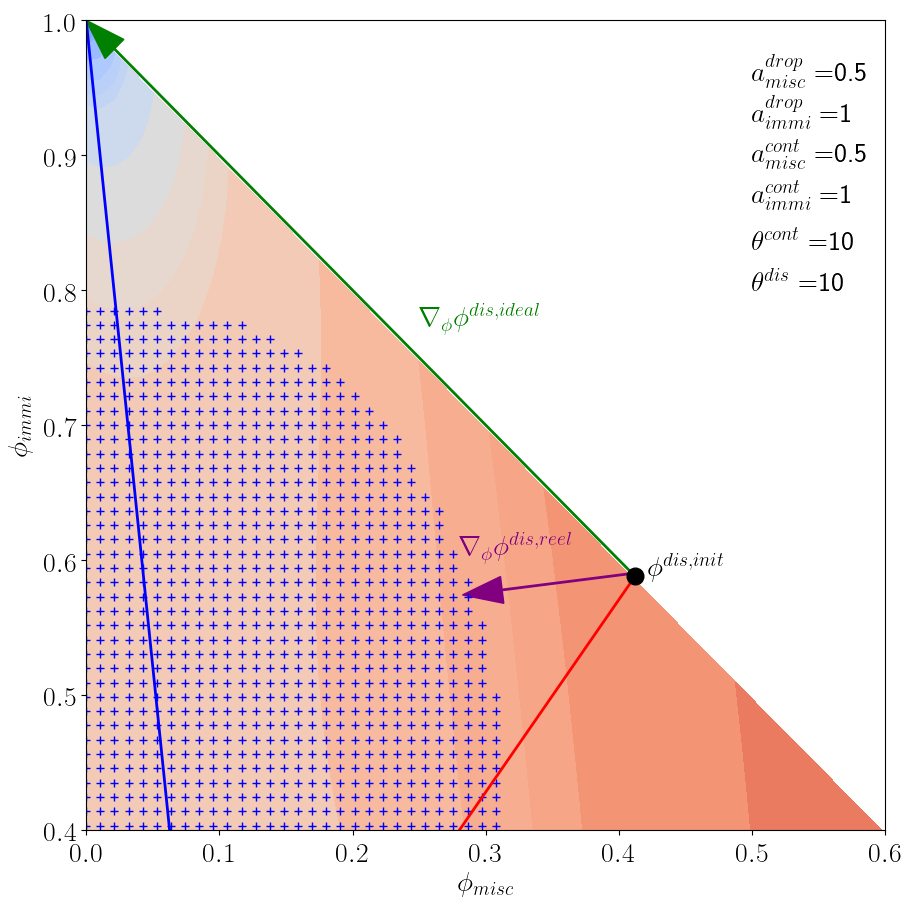
\includegraphics[width=\textwidth]{figure/direction_gradient}
 		\caption{Paysage thermodynamique partiel}
 		\label{fig:y equals x}
 	\end{subfigure}
 	\caption{Paysage thermodynamique et direction privilégiée par le système, la flèche verte représente le cas idéal sans intrusion d'eau et la flèche violette le cas associé au paysage thermodynamique, la zone bleu correspond à la zone instable}
 	\label{fig:paysage2}
 \end{figure}\vspace{-0.9cm}
 \begin{figure}[H]
 	\centering
 	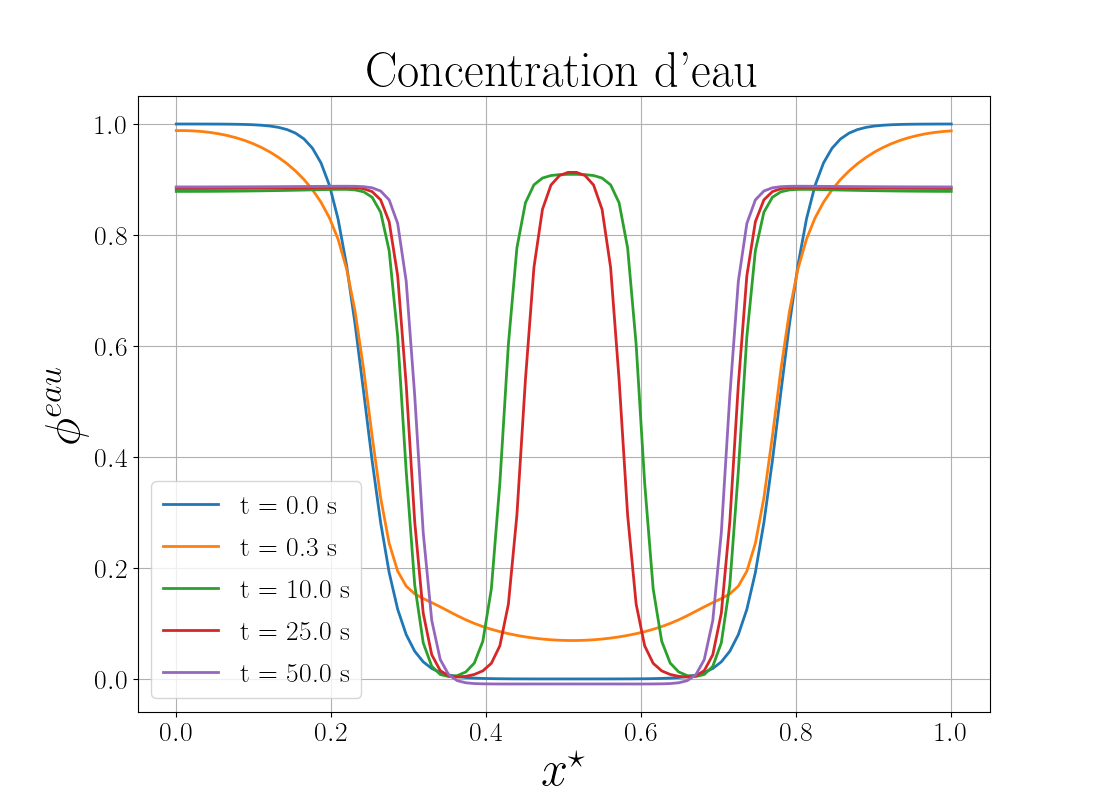
\includegraphics[width=0.7\linewidth]{figure/eau_ref}
 	\caption[Concentration d'eau dans le domaine]{Concentration d'eau dans le domaine, $x^{\star} = x / L_x$ représente une longueur adimensionnée}
 	\label{fig:eauref}
 \end{figure}\vspace{-0.7cm}
Finalement au travers de ces deux exemples, nous avons montré que pour qu'un paysage soit cohérent et potentiellement utilisable certaines conditions sont à remplir. Les critères concerne la position des conditions initiales, qui doivent être en dehors de la zone instable, un second critère concerne l'absence nécessaire de la zone instable sur le "chemin" de chacune des phases et finalement une direction initiale privilégiant une imperméabilité à l'eau dans la goutte.
\subsection{Validation d'un paysage}
Dans la suite on utilisera le paysage présenté en figure \ref{fig:thechoosenone} répondant à l'ensemble de ces critères.
\begin{figure}[H]
		\centering
		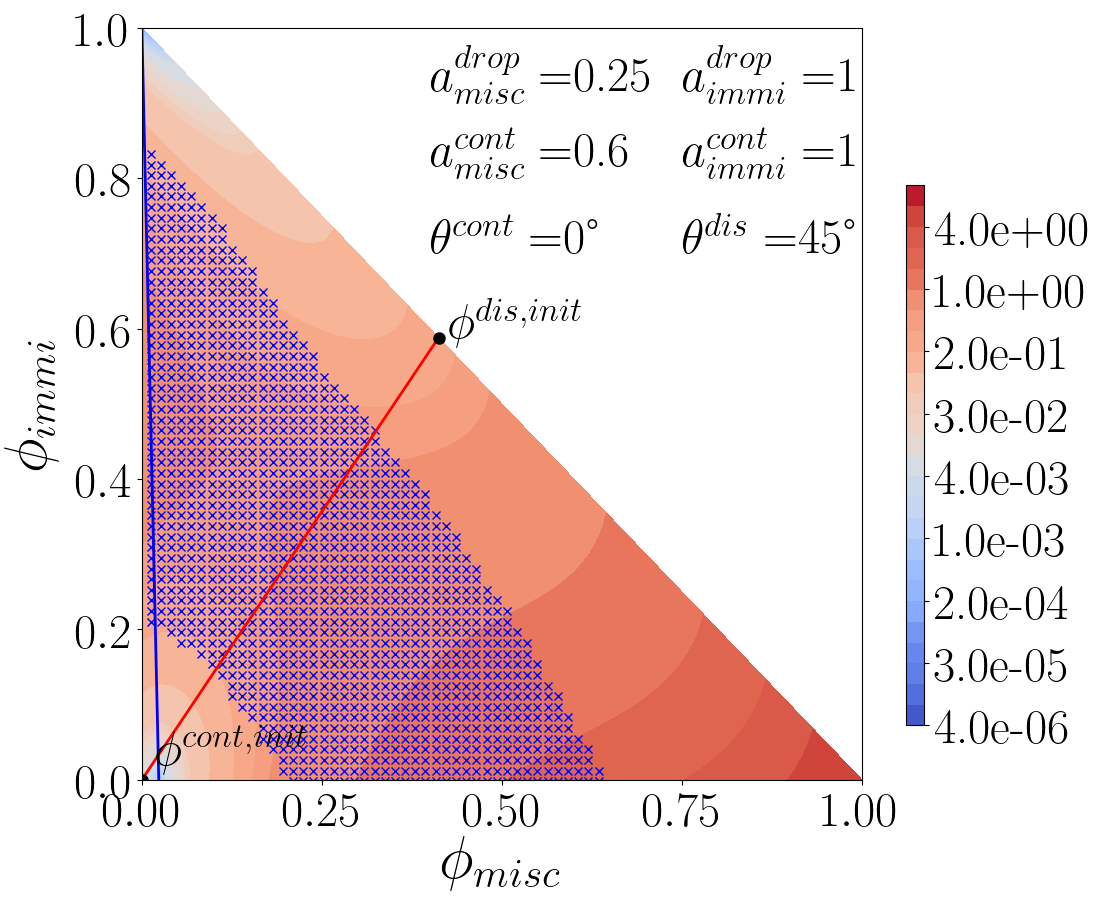
\includegraphics[width=0.45\textwidth]{figure/Paysage_ecriture1.png}
	\caption{Paysage thermodynamique choisit pour la simulation}
	\label{fig:thechoosenone}
\end{figure}

On cherche à tracer la solution stationnaire, sans couplage avec les équations de Navier-Stokes, on observe alors une non-monotonie de l'interface pour le composant miscible, de plus à l'intérieur de la goutte la concentration de composant miscible est négative et la composition d'élément immiscible est quant à elle supérieure à 1, de façon à obtenir une somme des deux concentrations égale à l'unité.
\begin{figure}[H]
	\centering
	\begin{subfigure}[H]{0.45\textwidth}
		\centering
		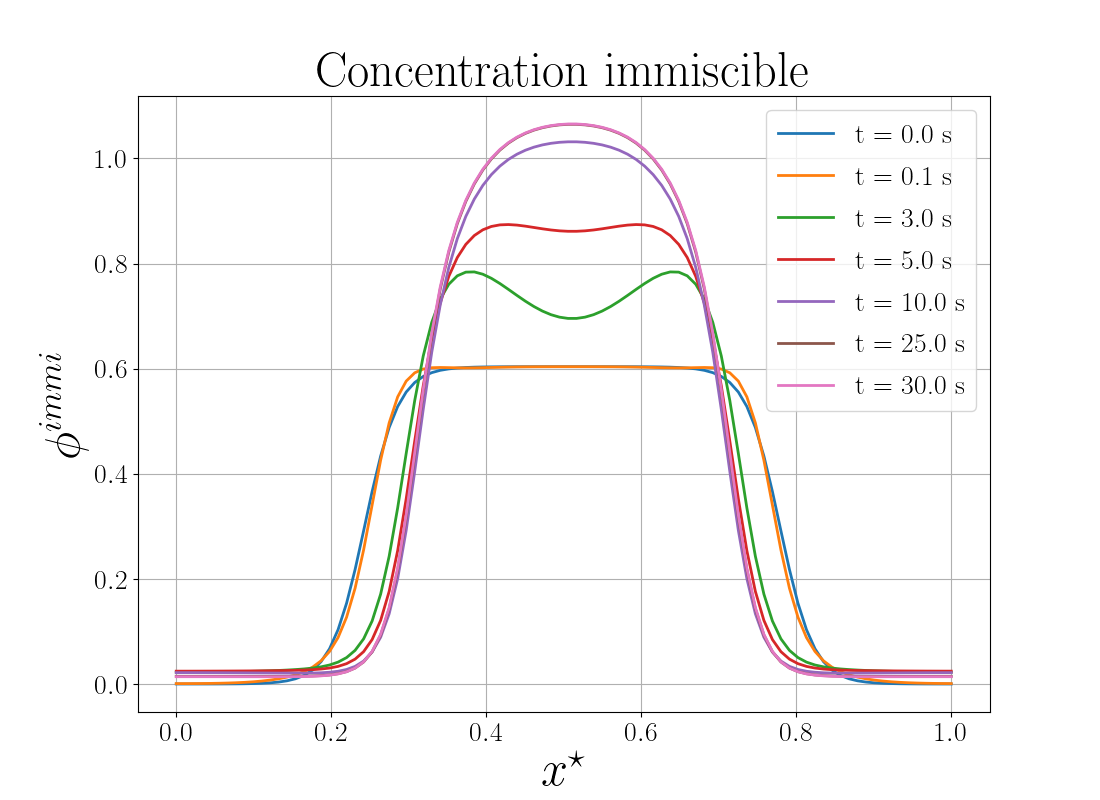
\includegraphics[width=\textwidth]{figure/nouveau_parametrage/immiscible_New_Parametrage.png}
		\caption{Concentration immiscible}
		\label{fig:y equals x}
	\end{subfigure}
	\hfill
	\begin{subfigure}[H]{0.45\textwidth}
		\centering
		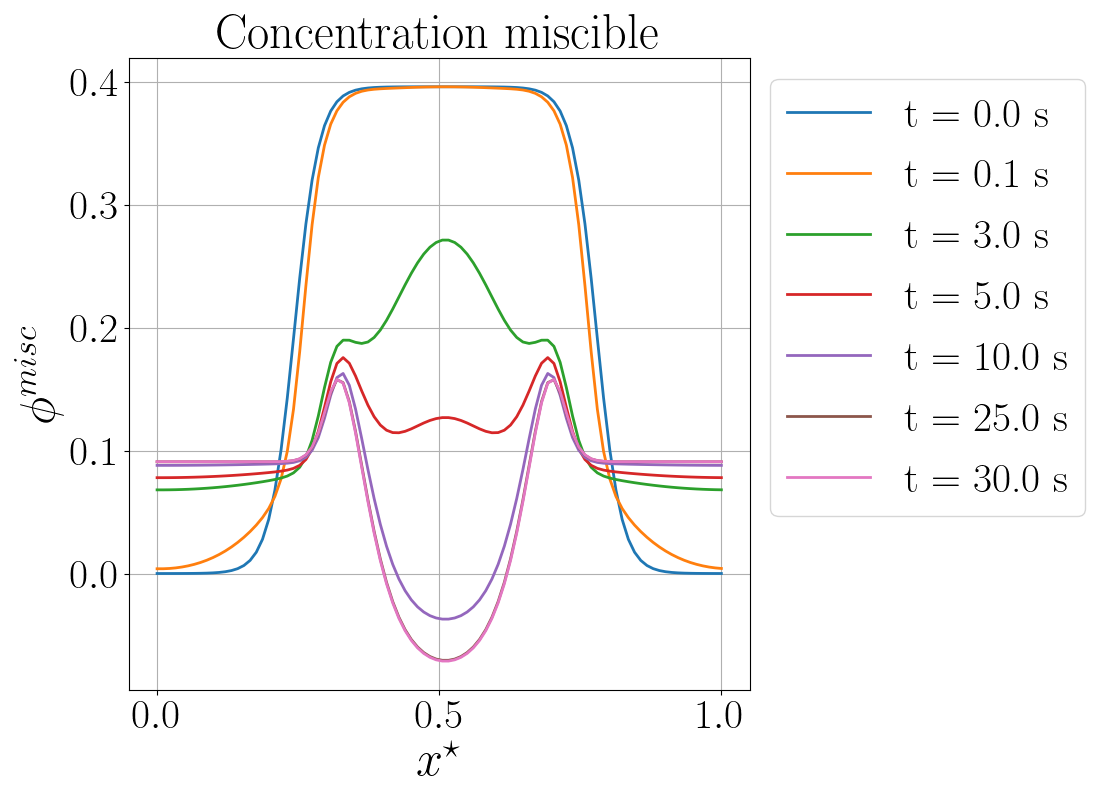
\includegraphics[width=\textwidth]{figure/nouveau_parametrage/miscible_New_Parametrage.png}
		\caption{Concentration miscible}
		\label{fig:y equals x}
	\end{subfigure}
\end{figure} \vspace{-0.8cm}
\begin{figure}[H]
	\centering
	\ContinuedFloat
	\begin{subfigure}[H]{0.45\textwidth}
		\centering
		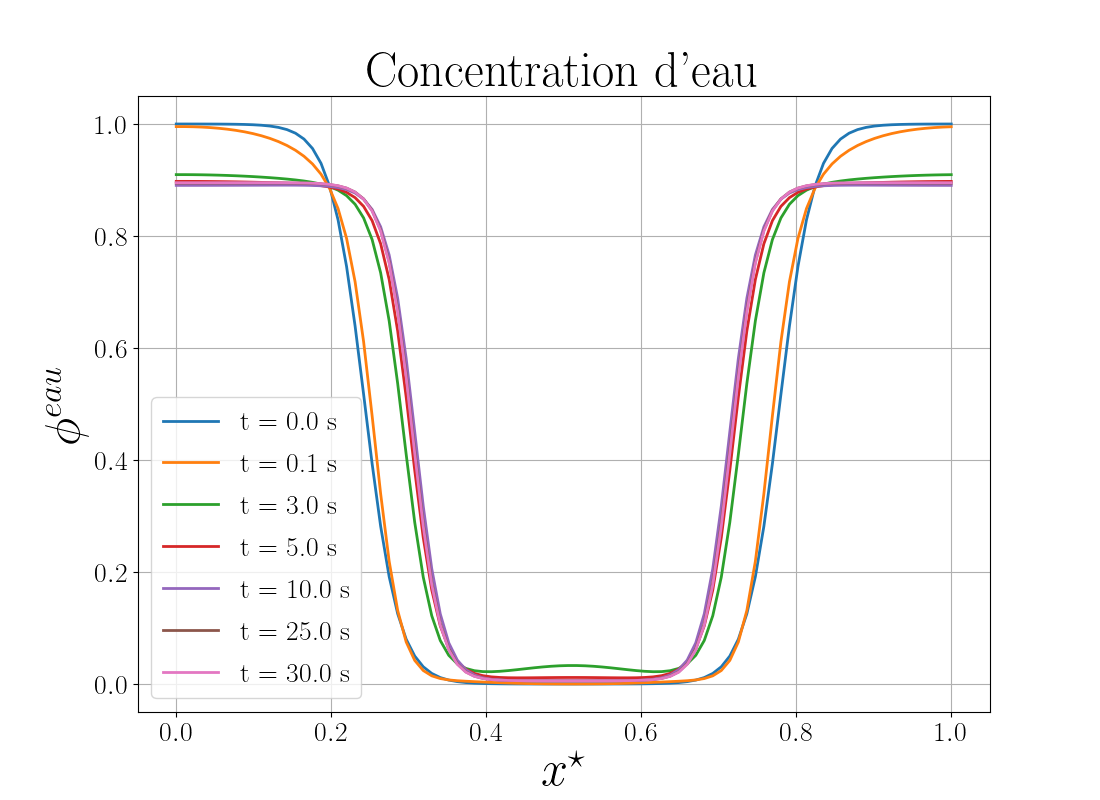
\includegraphics[width=\textwidth]{figure/nouveau_parametrage/eau_New_Parametrage.png}
		\caption{Concentration d'eau}
	\end{subfigure}
	\caption{Variation de la concentration des différents composants au cours du temps}
\end{figure}
On remarque alors une non-monotonie de l'interface. L'article \cite{rasolofomanana_diffuse-interface_2022} présente un paramétrisation du coefficient de gradient pour traiter les non monotonie d'interface, cette paramétrisation utilise la symétrie de la matrice coefficient de gradient pour la réécrire sous la forme :
\begin{equation}
\bar{\bar{\bm{\kappa}}} = \alpha \bm{R}\bm{D}\bm{R}^T
\label{eq:param_kappa}
\end{equation}
avec : $\bm{R}$ une matrice de rotation et $\bm{D}$ une matrice diagonale de la forme :
\begin{equation}
\bm{R} =    \begin{pmatrix} 
\cos\varphi & -\sin\varphi \\ 
\sin\varphi				&  \cos\varphi
\end{pmatrix}
\end{equation}
\begin{equation}
	\bm{D}(d) =    \begin{pmatrix} 
	2 & 0 \\ 
	0 & d
	\end{pmatrix} 
\end{equation}
La cohérence avec le système binaire est assurée par le coefficient $\alpha$ obtenu tel que :
\begin{equation}
\alpha = \frac{\kappa^{bin}}{2\cos^2\varphi + d \sin^2\varphi}
\end{equation}
On présente les différents résultats issus de la paramétrisation du coefficient de gradient : 
\begin{figure}[H]
		\centering
		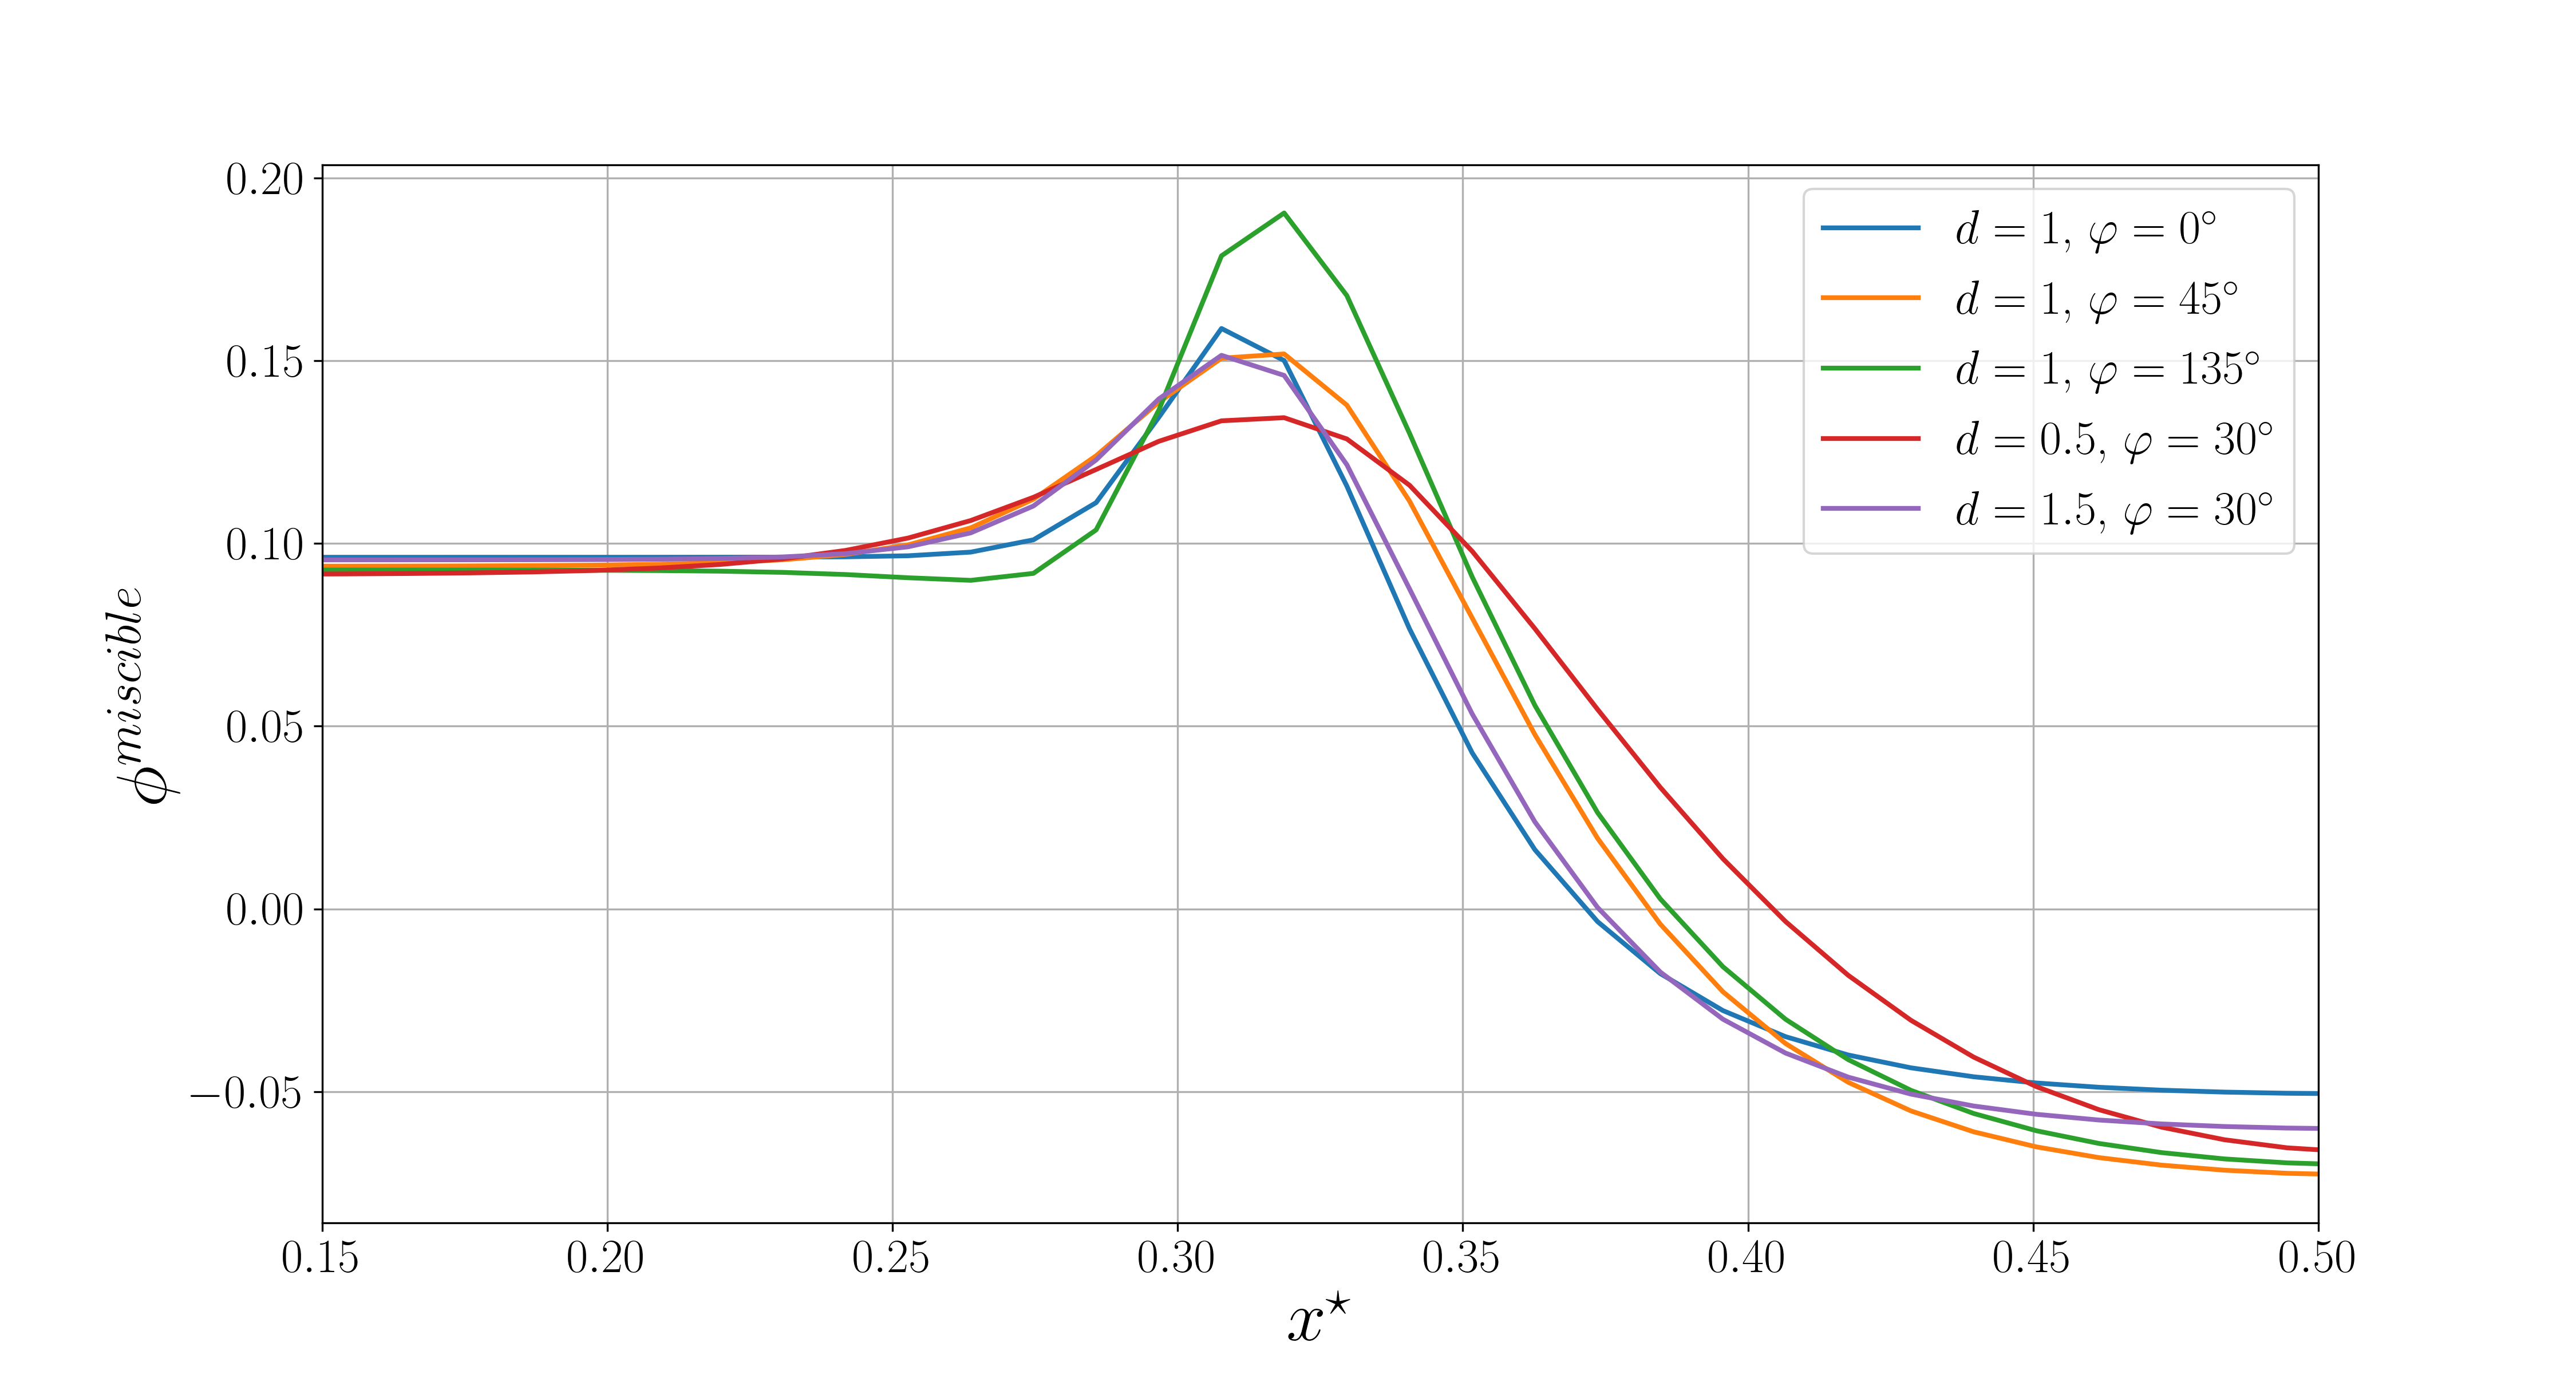
\includegraphics[width=0.7\textwidth]{figure/ProfInterfStatio2.png}
		\caption{Profils de l'interface pour différents paramétrages du coefficient de gradient}
\end{figure}


\chapter{Simulation du cas d'une goutte sans transfert de masse : exploration de différents régimes hydrodynamiques}
L'objectif de ce dernier chapitre est de démontrer la capacité du code à reproduire des comportements hydrodynamiques classique de la littérature. Une étude des différents régimes de déformation d'une goutte sera menée, la comparaison sera faite avec la corrélation de Clift et al. \cite{clift_bubbles_2005}.
\section{Rappel sur les nombres adimensionnés}
D'après Clift et al. \cite{clift_bubbles_2005} la déformation de la bulle est fonction des nombres adimensionnés de Reynolds, d'Eötvös et de Morton. On rappelle les valeurs de ces nombres adimensionnés : 
\begin{align}
\text{Re} &= \cfrac{\rho u D}{\eta}\\
\text{Eo} &= \cfrac{\Delta \rho g D^2}{\sigma}\\
\text{Mo} &= \cfrac{\Delta \rho g \eta^4}{\rho^2 \sigma^3}
\end{align}
avec $\rho$ la masse volumique du fluide porteur, $\Delta\rho = |\rho - \rho^{droplet}|$, $D$ le diamètre de la goutte. \\
L'étude de Clift et al. ayant été faite pour une goutte immiscible nous choisissons d'imposer une mobilité très faible de façon à rendre négligeable la diffusion.
Au vu des capacités de calculs disponible et des problèmes liés au développement présentés en section \ref{sec:difficulte} certains régimes ne sont pas atteignables.

\section{Conditions initiales et paramètres géométrique des simulations}
Les paramètres pour obtenir les différents régimes sont résumés dans le Tableau \ref{table:cas_ref_clift}. Les conditions initiales et la détermination de l'ensemble des coefficients restent inchangées par rapport au chapitre précédent. Le paysage choisit est le paysage présenté en Figure \ref{fig:landscapechap45}, ce paysage est celui utilisé dans \cite{rasolofomanana_numerical_nodate} et possède l'avantage de ne pas présenter de pathologie liée au profil d'interface.


\begin{figure}[H]
	\centering
	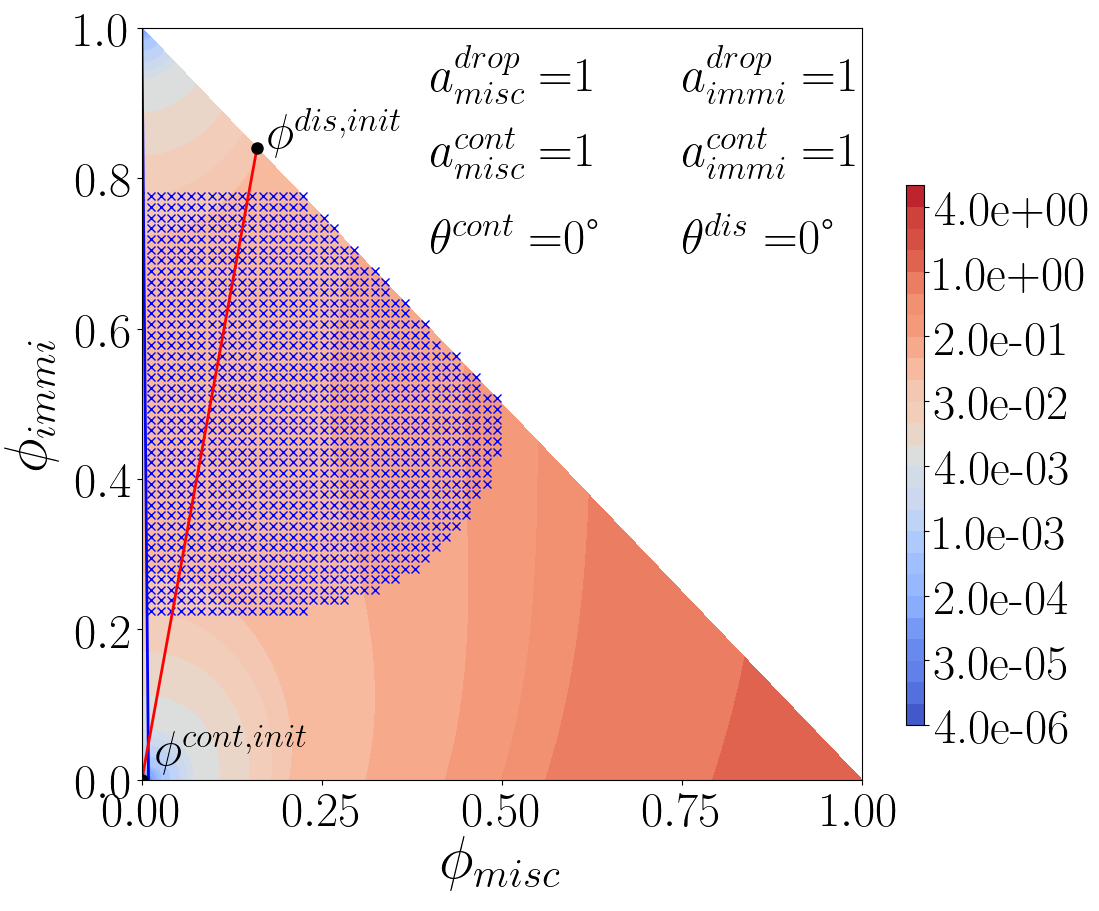
\includegraphics[width=0.5\linewidth]{figure/landscape_chap45}
	\caption{Paysage thermodynamique}
	\label{fig:landscapechap45}
\end{figure}

\begin{table}[H]
	\centering  % not needed, since table is as wide as text block
	\begin{tabularx}{\textwidth}{@{}lYYYYYY@{}}
		\toprule
		&\multicolumn{6}{c}{\bfseries Géométrie et maillage}\\
		%\cmidrule(lr){2-3} \cmidrule(l){4-5} 
		& $L_x$ (m)
		& $L_y$ (m)
		& $dx, dy$ (m)
		& $N_x$
		& $N_y$
		& $D^{drop}$  (m)\\
		\midrule
		Commun  & 7,35.10$^{-2}$ & 20.10$^{-2}$ & 2.10$^{-4}$ & 368 & 1000 & 9,8.10$^{-3}$ \\
		\bottomrule
	\end{tabularx}
\end{table} \vspace{-0.8cm}
\begin{table}[H]
	\begin{tabularx}{\textwidth}{@{}lYYYYYY@{}}
		\toprule
		&\multicolumn{6}{c}{\bfseries Paramètres physiques}\\
		%\cmidrule(lr){2-3} \cmidrule(l){4-5} 
		& $\rho^*$ (kg.m$^{-3}$)
		& $\eta$ (Pa.s)
		& $\beta_{misc}$ (-)
		& $\beta_{immi}$ (-)
		& $\epsilon$ (m)
		& $\sigma$ (N.m$^{-1}$)\\
		\midrule
		Spherical - Sphérique & 999,5 & 10$^{-1}$& -0,42 & 0,05 & 8.10$^{-4}$ & 36.10$^{-3}$ \\
		Ellipsoïdal - Elliptique & - & 14.10$^{-3}$& - & - & - & 2.10$^{-3}$ \\
		Dimpled - Creusé & - & 10$^{-1}$& - & - & - & 10$^{-4}$ \\
		Skirted - Juppé & - & 13.10$^{-3}$& - & - & - & 4.10$^{-5}$ \\
		\bottomrule
	\end{tabularx}
\end{table}\vspace{-0.8cm}
\begin{table}[H]
	\begin{tabularx}{\textwidth}{@{}lYYYYYY@{}}
		\toprule
		&\multicolumn{5}{c}{\bfseries Paramètres "champ de phase" et nombres sans dimension}\\
		%\cmidrule(lr){2-3} \cmidrule(l){4-5} 
		& $\lambda$ (-)
		& $\kappa$
		& $\mathcal{M}$ (m$^2$.s$^{-1}$)
		& Eo
		& log(Mo)\\
		\midrule
		Spherical - Sphérique  & 540 & 4,32.10$^{-5}$ $\delta_{ij}$ & 1.10$^{-13}$ $\delta_{ij}$ & 0,65 & -3\\	
		Ellipsoïdal - Elliptique  & 30 & 2,4.10$^{-6}$ $\delta_{ij}$ & - &12 & -3 \\	
		Dimpled - Creusé  & 1,5 & 1,2.10$^{-7}$ $\delta_{ij}$ & - &235 & 4,3 \\
		Skirted - Juppé  & 0,6 & 4,8.10$^{-8}$ $\delta_{ij}$ & - & 588 & 2 \\
		\bottomrule
	\end{tabularx}
\end{table}\vspace{-0.8cm}
\begin{table}[H]
	\begin{tabularx}{\textwidth}{@{}lYYYYYYYY@{}}
		\toprule
		&\multicolumn{8}{c}{\bfseries Conditions initiales et d'équilibres}\\
		%\cmidrule(lr){2-3} \cmidrule(l){4-5} 
		& $\phi_{misc}^{drop}$ 
		& $\phi_{immi}^{drop}$ 
		& $\phi_{misc}^{cont}$ 
		& $\phi_{immi}^{cont}$
		& $\phi_{misc}^{drop,eq}$ 
		& $\phi_{immi}^{drop,eq}$ 
		& $\phi_{misc}^{cont,eq}$ 
		& $\phi_{immi}^{cont,eq}$ \\
		\midrule
		Commun  & 0,16 & 0,84 & 0 & 0 & 0 & 1 & 8.10$^{-4}$ & 0\\
		\bottomrule
	\end{tabularx}
	\caption{Paramètres des simulations} \label{table:cas_ref_clift}
\end{table}

%\begin{center}
%	\begin{tabular}{|c||c|c|c|c|}
%		\hline 
%		Régime & Spherical & Ellipsoïdal & Dimpled & Skirted \\ 
%		\hline  \hline
%		Viscosité dynamique $\eta$ (Pa.s) & 0,1 & 0,014 & 0,1 & 0,013  \\ 
%		\hline 
%		Tension de surface $\sigma$ (N.m$^{-1}$)& 36.10$^{-3}$ &2.10$^{-3}$ & 1.10$^{-4}$ & 4.10$^{-5}$ \\ 
%		\hline 
%		Coefficient de gradient d'énergie $\kappa$ (N.m$^{-2}$) & 4,32.10$^{-5}$ & 2,4.10$^{-6}$ & 1,2.10$^{-7}$ & 4,8.10$^{-8}$  \\ 
%		\hline 
%		Coefficient d'upscaling (-) & 540 & 30 & 1,5  & 0,6  \\ 
%		\hline 
%		Nombre d'Eötvös & 0.65 & 11,77 & 235,53 & 588,84 \\ 
%		\hline 
%		Logarithme du nombre de Morton & -3 & -3 & 4,4 & 2  \\ 
%		\hline 
%	\end{tabular} 
%\end{center}
\section{Résultats}
Les résultats des simulations sont présentés en Figure \ref{fig:abaque}, on y retrouve 4 régimes de déformation de la goutte. Il est possible d'observer que les différents régimes sont globalement retranscrits. Cependant, il ne faut pas perdre de vue les problématiques liées à la convergence du maillage. Concernant les résultats obtenus, le régime \textit{skirted} est instable. Cette instabilité semble provenir du caractère diffus de l'interface détachant des "poches" de matière lorsque l'épaisseur de la jupe est trop fine. Ce phénomène est présent sur l'ensemble des résultats, en effet la séparation d'échelle entre l'épaisseur de l'interface est la goutte ne permet pas d'avoir des résultats plus cohérents.
\begin{figure}[H]
	\centering
	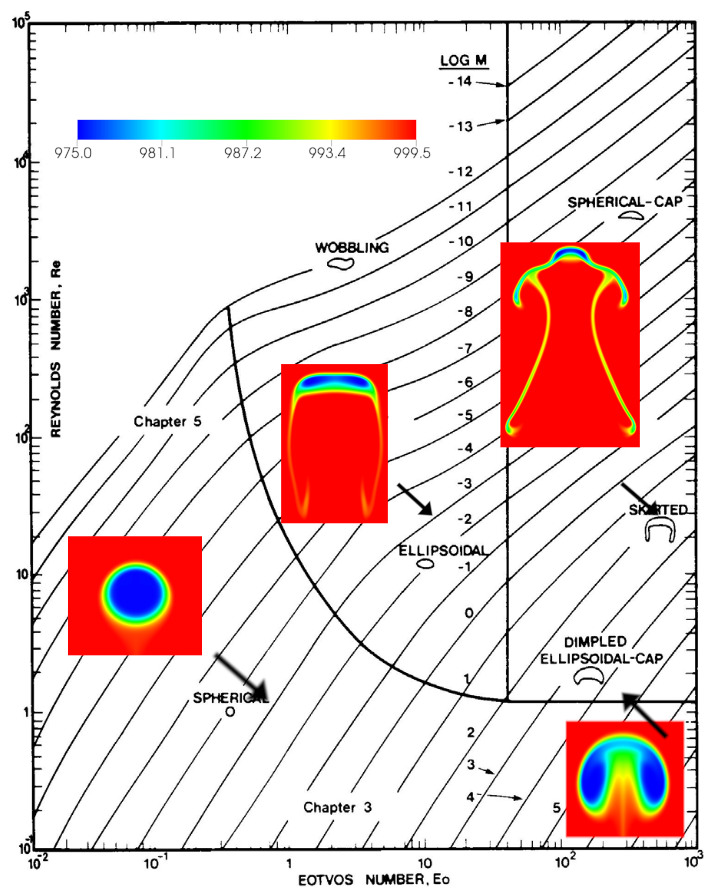
\includegraphics[width=1.0\linewidth]{figure/projet_abaque.png}
	\caption{Déformation du goutte, d'après \cite{clift_bubbles_2005}, \textcolor{blue}{je vais refaire la figure avec une seule colorbar suffisamment grosse}}
	\label{fig:abaque}
\end{figure}




 
\chapter{Simulation d'une inversion de stratification associée au transfert de masse}

Pour conclure l'étude, on cherche à modéliser le détachement de gouttelettes induites par transfert de masse. Le détachement est un cas important d'étude puisque c'est un phénomène déterminant pour l'étude de la stratification du bain de corium (\textit{cf.} Chapitre \ref{chap:1}). L'analyse du régime linéaire d'une instabilité de Rayleigh-Taylor dans TrioCFD a été effectuée dans \cite{rasolofomanana_modelisation_nodate} avec des résultats tout à fait satisfaisants. Ainsi, l'objectif de cette section est simplement d'observer un détachement de gouttelettes dans un système ternaire et une relocalisation en fond de domaine.
\section{Conditions initiales}
Le paysage choisi est la même que celui utilisé au chapitre précédent en notant les phases $\alpha$ et $\beta$, il est représenté en Figure \ref{fig:landchap5}, une fois de plus ce paysage nous conserve de tout problème lié au profil d'interface. Un schéma représentatif des conditions initiales est présenté en Figure \ref{fig:schema_RT}, initialement la phase $\alpha$ est plus légère que la phase $\beta$, puis sous l'effet de la diffusion de l'élément léger de la phase $\alpha$ vers la phase $\beta$, la phase $\alpha$ s'alourdit jusqu'au détachement de gouttelettes.	

\begin{figure}[H]
	\centering
\begin{subfigure}[ht!]{0.45\textwidth}
		\centering
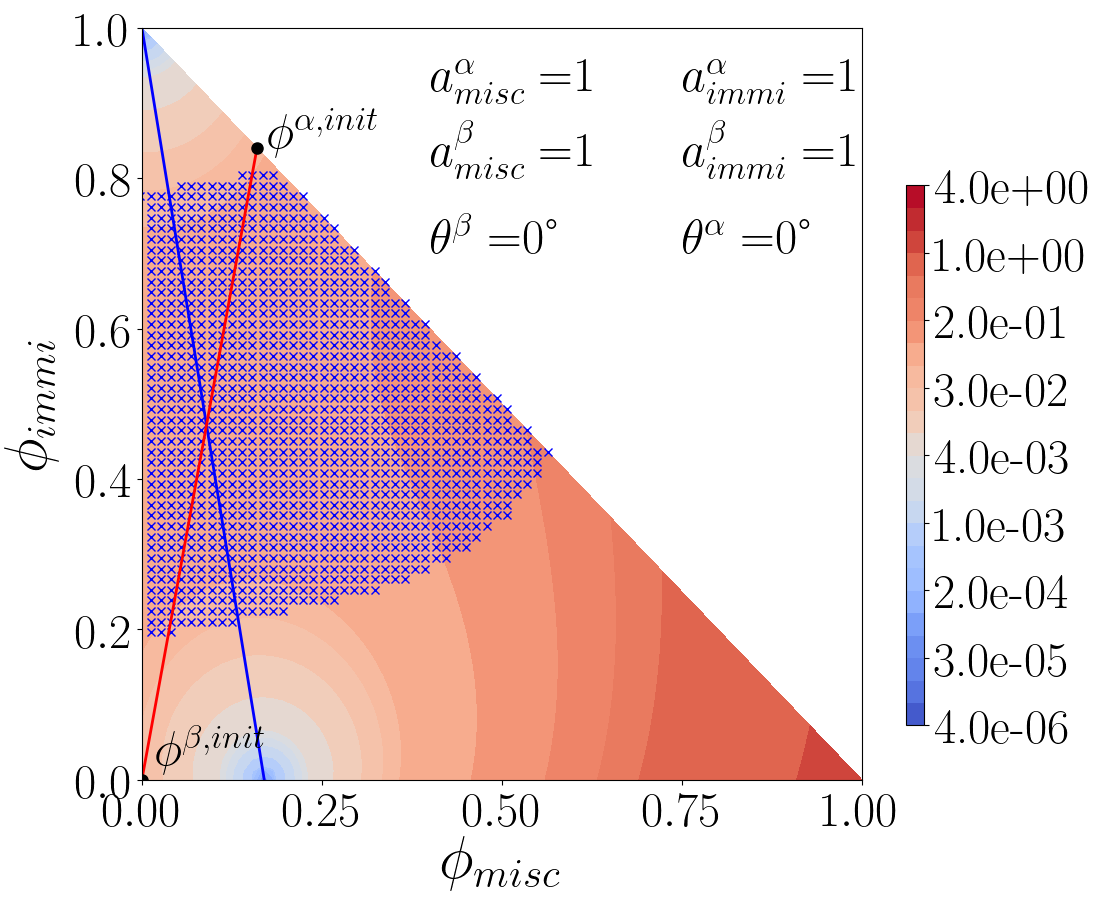
\includegraphics[width=1\textwidth]{figure/landscape_chap5.png}
\caption{Paysage thermodynamique}
\label{fig:landchap5}
\end{subfigure}
\begin{subfigure}[ht!]{0.45\textwidth}
	\centering
\begin{circuitikz}[scale=0.4]
	%		\oeil[shift={(3.5,5.2)},rotate=60,fill=white];
	%		\draw [-triangle 60] (4,6) -- (6,9);
	\begin{scope}[xshift=3cm]
		\draw [scale=1,thick] (0,0) -- (6,0) -- (6,12) -- (0,12) -- cycle;
		\draw [scale=1,thick] (0,9) -- (6,9) ;
		%\draw [scale=1,thick,dashed] (3,8) -- (3,10) ;
		\draw [scale=1,thick,dashed] (3,9) circle (0.8cm) node {};
		\draw [-triangle 60] (4,6) -- (3,9);
		\node (A) at (4,5) {perturb.};
		\node (A) at (3,1.7) {phase $\beta$};
		\node (B) at (3,11) {phase $\alpha$};
	\end{scope}
\end{circuitikz}
\caption{Schéma représentatif des conditions initiales}
\label{fig:schema_RT}
\end{subfigure}
\caption{Schéma représentatif des conditions initiales et paysage thermodynamique}
\label{fig:schema_RTetlandscape}
\end{figure}
Les simulations sont réalisées sur un système non-physique, ainsi, tout comme le paysage, la tension de surface et la viscosité sont choisies arbitrairement, la viscosité est cohérente avec le cas du corium, cependant la tension de surface est cinquante fois plus faible que l'ordre de grandeur de référence du corium. Les dimensions du système sont également fortement réduite par rapport à une cuve. Cependant les dimensions se rapprochent des essais mettant en jeu du corium prototypique en creuset froid MASCA-MA avec un creuset de 7cm de diamètre pour 2kg de corium, au cours desquels les inversions sont très rapide (<30 minutes). Les paramètres de la simulation sont présentés en Tableau \ref{table:cas_ref_RT}.
\begin{table}[H]
	\centering  % not needed, since table is as wide as text block
	\begin{tabularx}{\textwidth}{@{}lYYYYYY@{}}
		\toprule
		&\multicolumn{6}{c}{\bfseries Géométrie et maillage}\\
		%\cmidrule(lr){2-3} \cmidrule(l){4-5} 
		& $L_x$ (m)
		& $L_y$ (m)
		& $dx, dy$ (m)
		& $N_x$
		& $N_y$
		& $y_0$  (m)\\
		\midrule
		Valeurs  & 3.10$^{-2}$ & 5.10$^{-2}$ & 2.10$^{-4}$ & 150 & 500 & 0,037 \\
		\bottomrule
	\end{tabularx}
\end{table} \vspace{-0.8cm}
\begin{table}[H]
	\begin{tabularx}{\textwidth}{@{}lYYYYYY@{}}
		\toprule
		&\multicolumn{5}{c}{\bfseries Paramètres physiques}\\
		%\cmidrule(lr){2-3} \cmidrule(l){4-5} 
		& $\rho^*$ (kg.m$^{-3}$)
		& $\eta$ (Pa.s)
		& $\beta_{misc}$ (-)
		& $\beta_{immi}$ (-)
		& $\epsilon$ (m)\\
		\midrule
		Valeurs & 999,5 & 10$^{-3}$& -0,42 & 0,05 & 8.10$^{-4}$ \\
		\bottomrule
	\end{tabularx}
\end{table}\vspace{-0.8cm}
\begin{table}[H]
	\begin{tabularx}{\textwidth}{@{}lYYYY@{}}
		\toprule
		&\multicolumn{3}{c}{\bfseries Paramètres "champ de phase"}\\
		%\cmidrule(lr){2-3} \cmidrule(l){4-5} 
		& $\lambda$ (-)
		& $\kappa$
		& $\mathcal{M}$ (m$^2$.s$^{-1}$) \\
		\midrule
		Valeurs  & 27 & 2,16.10$^{-6}$ $\delta_{ij}$ & 1.10$^{-8}$ $\delta_{ij}$ \\	
		\bottomrule
	\end{tabularx}
\end{table}\vspace{-0.8cm}
\begin{table}[H]
	\begin{tabularx}{\textwidth}{@{}lYYYYYYYY@{}}
		\toprule
		&\multicolumn{8}{c}{\bfseries Conditions initiales et d'équilibres}\\
		%\cmidrule(lr){2-3} \cmidrule(l){4-5} 
		& $\phi_{misc}^{drop}$ 
		& $\phi_{immi}^{drop}$ 
		& $\phi_{misc}^{cont}$ 
		& $\phi_{immi}^{cont}$
		& $\phi_{misc}^{drop,eq}$ 
		& $\phi_{immi}^{drop,eq}$ 
		& $\phi_{misc}^{cont,eq}$ 
		& $\phi_{immi}^{cont,eq}$ \\
		\midrule
		Commun  & 0,12 & 0,87 & 0 & 0 & 0 & 1 & 0,17 & 0\\
		\bottomrule
	\end{tabularx}
	\caption{Paramètres des simulations} \label{table:cas_ref_RT}
\end{table}
Les conditions initiales de concentration peuvent s'écrire sous la forme :
\begin{equation}
\phi_{i}(\mathbf{x},t=0) = \frac{\phi^{init,\beta}_i + \phi^{init,\alpha}_i  }{2} +  \frac{\phi^{init,\beta}_i - \phi^{init,\alpha}_i }{2}\tanh\left(\frac{y-y_0+\gamma_1\exp\left(-\gamma_2 \text{rnd}\left(\cfrac{L_x}{2}-abs(x)\right)\right)}{\epsilon}\right)
\end{equation}
avec $\gamma_1, \gamma_2$ deux constantes, rnd$(u)$ un nombre pseudo-aléatoire compris entre $0$ et $u$, $L_x$ la largeur du domaine et $y_0$ la position de l'interface.\\
L'introduction de cette perturbation permet d'éviter le développement d'une instabilité mono-mode, de plus, sous l'effet de la diffusion initiale, permet d'introduire une excitation plus réaliste de l'interface.
\section{Résultats}
Les résultats sont présentés en Figure \ref{fig:rt1}, \ref{fig:rt2} et \ref{fig:rt3}. On y retrouve bien un détachement de gouttelettes menant à une inversion totale et une relocalisation en fond de domaine. Cependant, il est également possible d'observer que les parois du domaine semblent perturber légèrement le système. La Figure \ref{fig:profrhort} permet d'observer la diffusion massique dès les premiers instants du calcul menant à ce détachement de gouttelette.
\begin{figure}[H]
	\centering
	\begin{subfigure}[ht!]{0.2\textwidth}
		\centering
		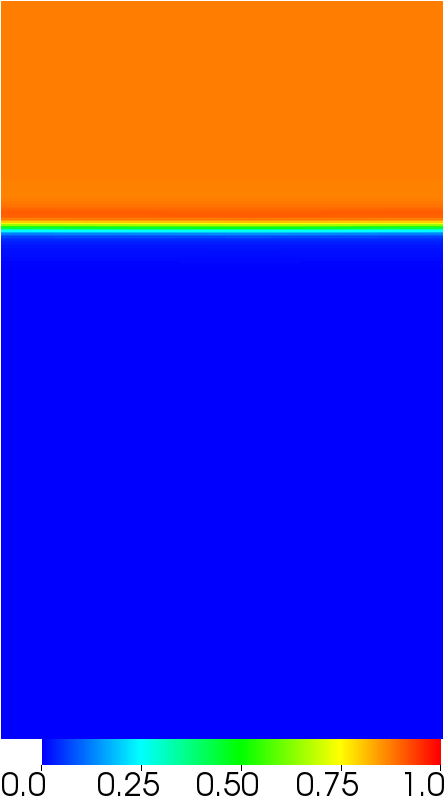
\includegraphics[width=1\textwidth]{figure/PT_RT/concent1/visit0000.png}
		\caption{$t=1s$}
	\end{subfigure}
	\begin{subfigure}[ht!]{0.2\textwidth}
		\centering
		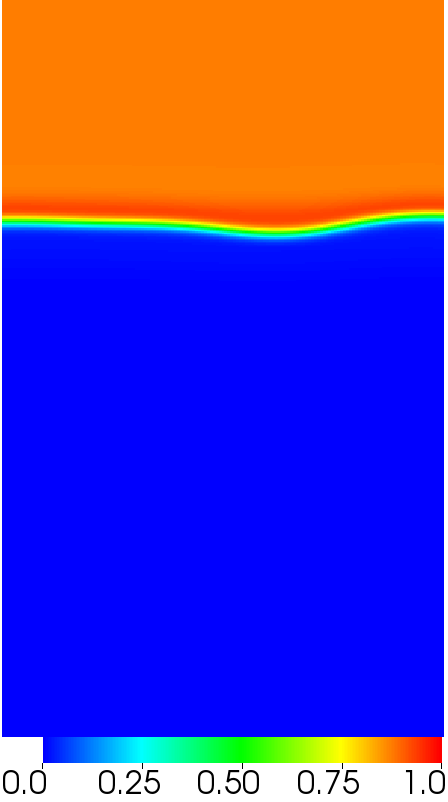
\includegraphics[width=1\textwidth]{figure/PT_RT/concent1/visit0001.png}
		\caption{$t=2s$}
	\end{subfigure}
	\begin{subfigure}[ht!]{0.2\textwidth}
		\centering
		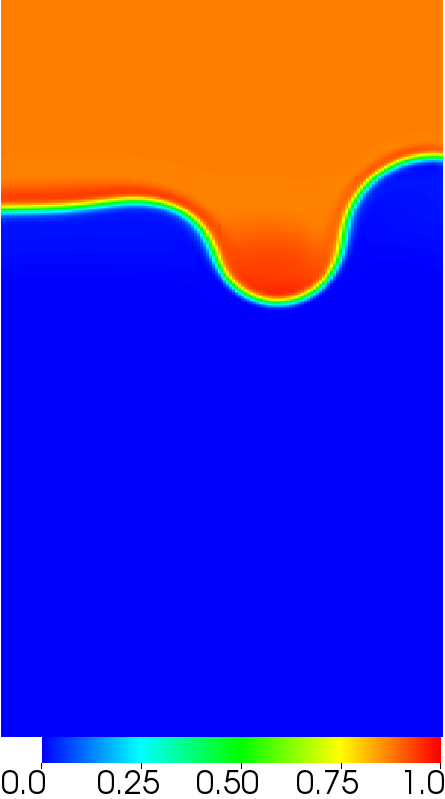
\includegraphics[width=1\textwidth]{figure/PT_RT/concent1/visit0002.png}
		\caption{$t=2,5s$}
	\end{subfigure}
	\begin{subfigure}[ht!]{0.2\textwidth}
		\centering
		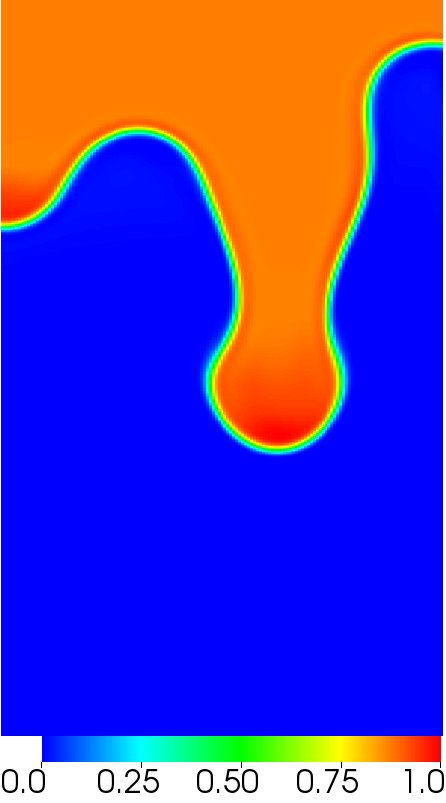
\includegraphics[width=1\textwidth]{figure/PT_RT/concent1/visit0003.png}
		\caption{$t=3s$}
	\end{subfigure}
\end{figure}\vspace{-0.8cm}
\begin{figure}[H]
	\centering
	\ContinuedFloat
	\begin{subfigure}[ht!]{0.2\textwidth}
		\centering
		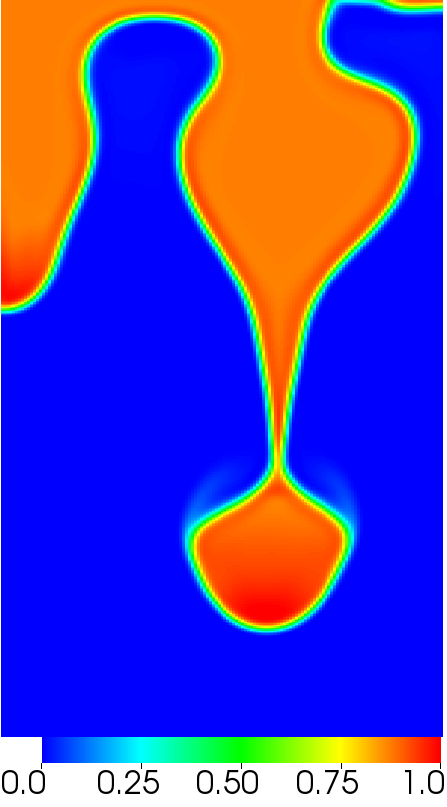
\includegraphics[width=1\textwidth]{figure/PT_RT/concent1/visit0004.png}
		\caption{$t=3,5s$}
	\end{subfigure}
	\begin{subfigure}[ht!]{0.2\textwidth}
		\centering
		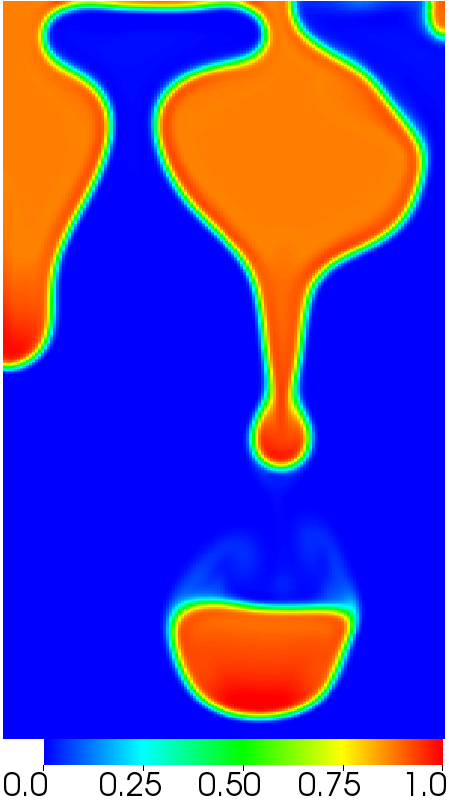
\includegraphics[width=1\textwidth]{figure/PT_RT/concent1/visit0005.png}
		\caption{$t=3,75s$}
	\end{subfigure}
	\begin{subfigure}[ht!]{0.2\textwidth}
		\centering
		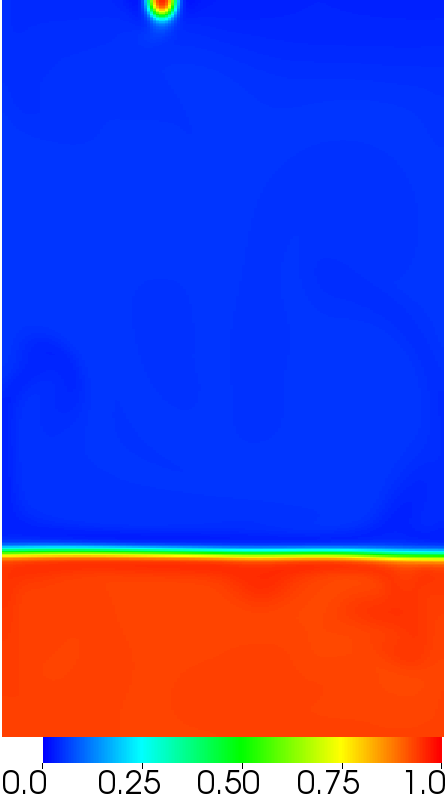
\includegraphics[width=1\textwidth]{figure/PT_RT/concent1/visit0006.png}
		\caption{$t=40s$}
	\end{subfigure}
	\caption{Champ de concentration de l'élément immiscible}
	\label{fig:rt1}
\end{figure}


\begin{figure}[H]
	\centering
	\begin{subfigure}[ht!]{0.2\textwidth}
		\centering
		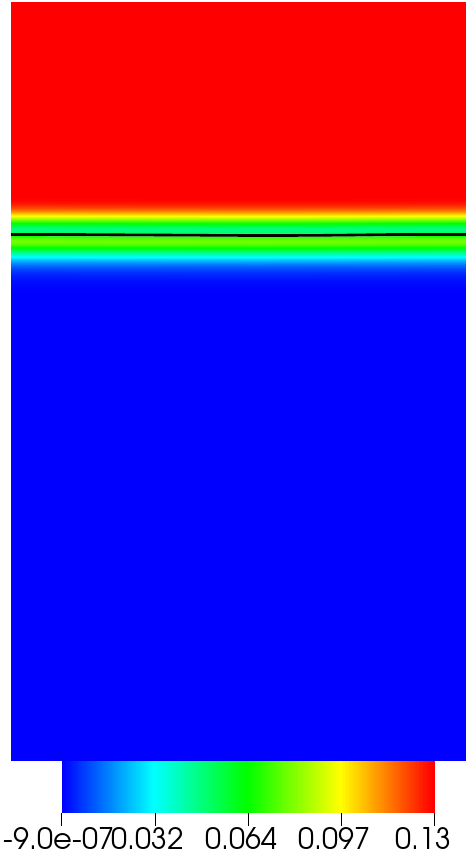
\includegraphics[width=1\textwidth]{figure/PT_RT/concent0/visit0007.png}
		\caption{$t=1s$}
	\end{subfigure}
	\begin{subfigure}[ht!]{0.2\textwidth}
		\centering
		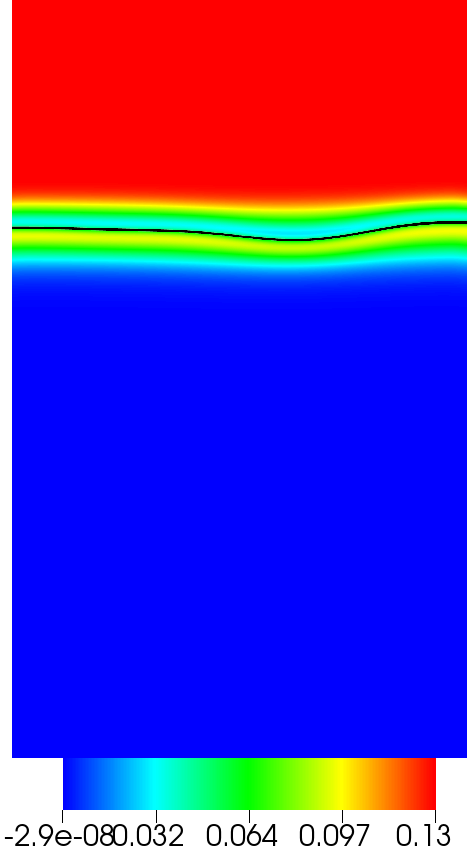
\includegraphics[width=1\textwidth]{figure/PT_RT/concent0/visit0008.png}
		\caption{$t=2s$}
	\end{subfigure}
	\begin{subfigure}[ht!]{0.2\textwidth}
		\centering
		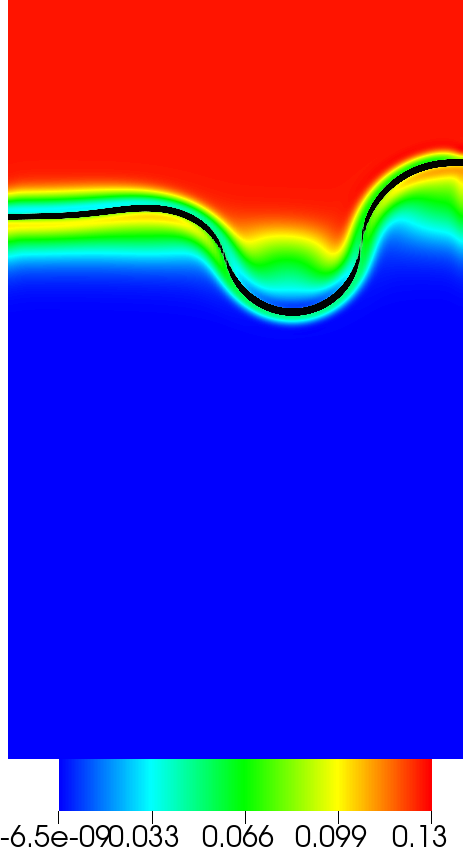
\includegraphics[width=1\textwidth]{figure/PT_RT/concent0/visit0009.png}
		\caption{$t=2,5s$}
	\end{subfigure}
	\begin{subfigure}[ht!]{0.2\textwidth}
		\centering
		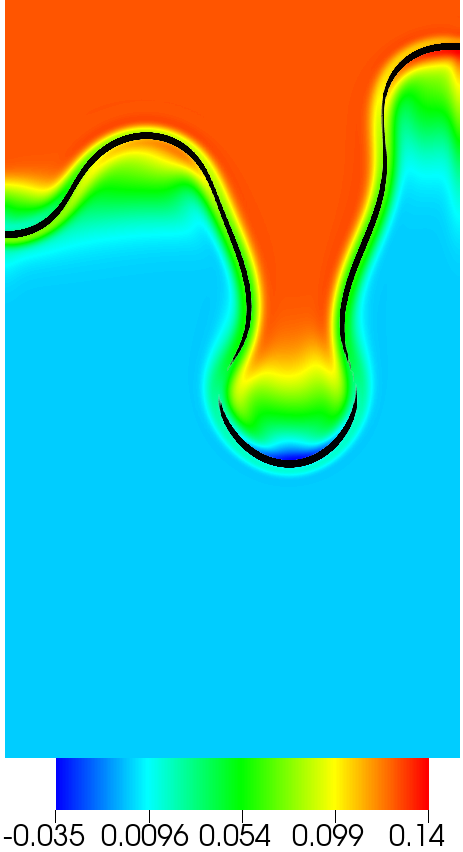
\includegraphics[width=1\textwidth]{figure/PT_RT/concent0/visit0010.png}
		\caption{$t=3s$}
	\end{subfigure}
\end{figure}\vspace{-0.8cm}
\begin{figure}[H]
	\centering
	\ContinuedFloat
	\begin{subfigure}[ht!]{0.2\textwidth}
		\centering
		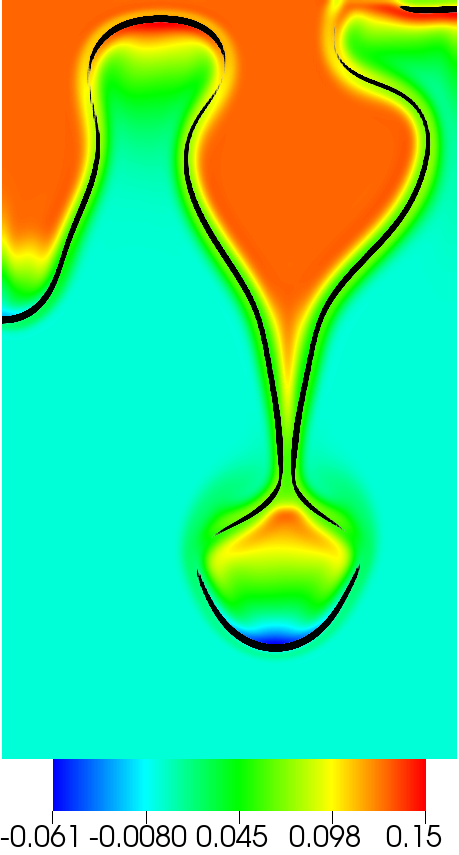
\includegraphics[width=1\textwidth]{figure/PT_RT/concent0/visit0011.png}
		\caption{$t=3,5s$}
	\end{subfigure}
	\begin{subfigure}[ht!]{0.2\textwidth}
		\centering
		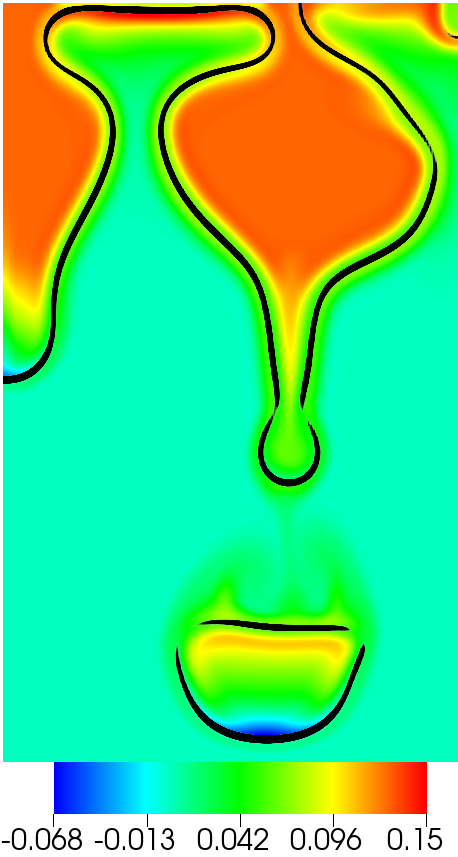
\includegraphics[width=1\textwidth]{figure/PT_RT/concent0/visit0012.png}
		\caption{$t=3,75s$}
	\end{subfigure}
	\begin{subfigure}[ht!]{0.2\textwidth}
		\centering
		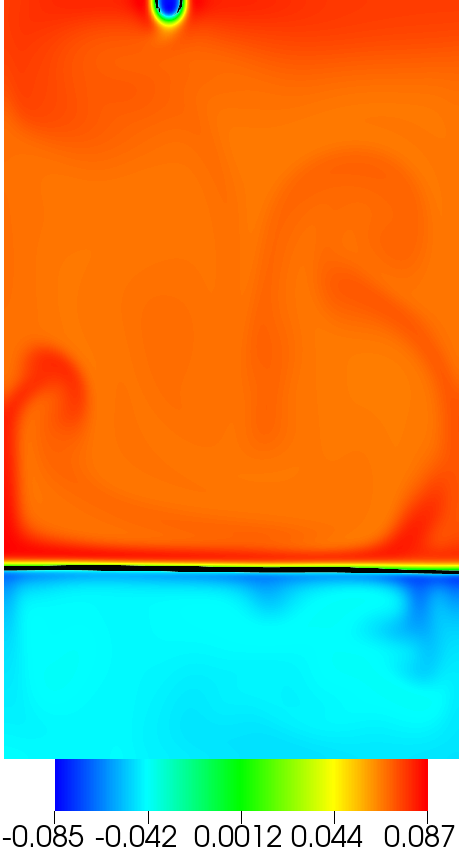
\includegraphics[width=1\textwidth]{figure/PT_RT/concent0/visit0013.png}
		\caption{$t=40s$}
	\end{subfigure}
	\caption{Champ de concentration de l'élément miscible}
	\label{fig:rt2}
\end{figure}


\begin{figure}[H]
	\centering
	\begin{subfigure}[ht!]{0.2\textwidth}
		\centering
		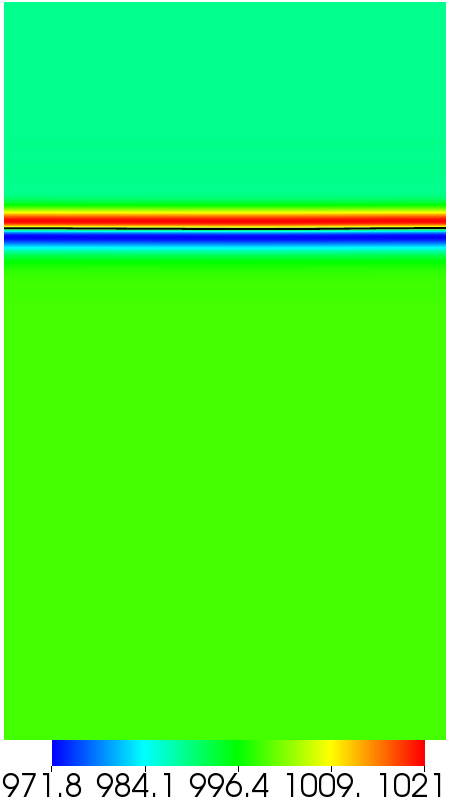
\includegraphics[width=1\textwidth]{figure/PT_RT/masse_vol/visit0014.png}
		\caption{$t=1s$}
	\end{subfigure}
	\begin{subfigure}[ht!]{0.2\textwidth}
		\centering
		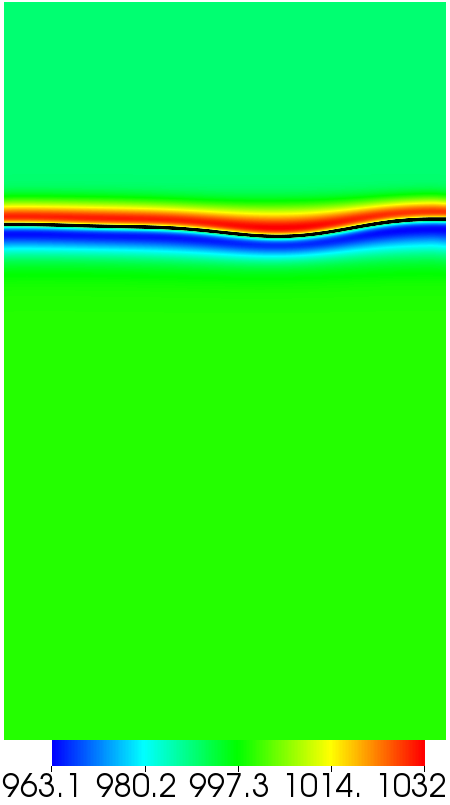
\includegraphics[width=1\textwidth]{figure/PT_RT/masse_vol/visit0015.png}
		\caption{$t=2s$}
	\end{subfigure}
	\begin{subfigure}[ht!]{0.2\textwidth}
		\centering
		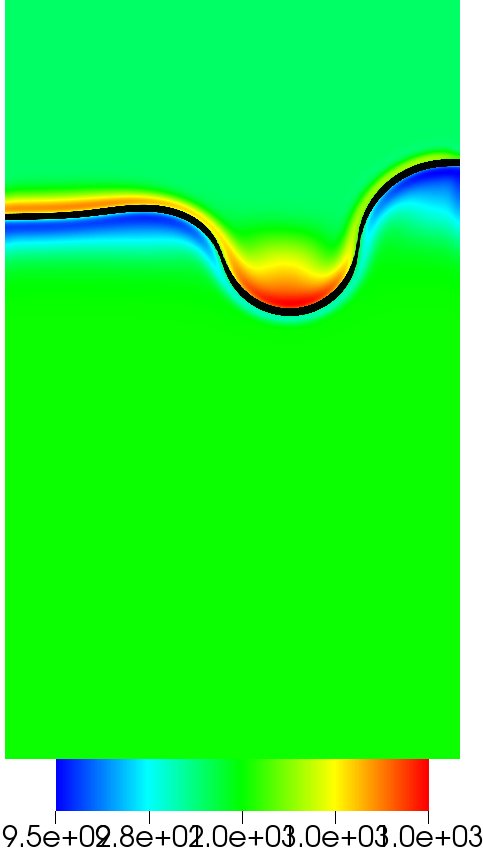
\includegraphics[width=1\textwidth]{figure/PT_RT/masse_vol/visit0020.png}
		\caption{$t=2,5s$}
	\end{subfigure}
	\begin{subfigure}[ht!]{0.2\textwidth}
		\centering
		\includegraphics[width=1\textwidth]{figure/PT_RT/masse_vol/visit0016.png}
		\caption{$t=3s$}
	\end{subfigure}
\end{figure}\vspace{-0.8cm}
\begin{figure}[H]
	\centering
	\ContinuedFloat
	\begin{subfigure}[ht!]{0.2\textwidth}
		\centering
		\includegraphics[width=1\textwidth]{figure/PT_RT/masse_vol/visit0017.png}
		\caption{$t=3,5s$}
	\end{subfigure}
	\begin{subfigure}[ht!]{0.2\textwidth}
		\centering
		\includegraphics[width=1\textwidth]{figure/PT_RT/masse_vol/visit0018.png}
		\caption{$t=3,75s$}
	\end{subfigure}
	\begin{subfigure}[ht!]{0.2\textwidth}
		\centering
		\includegraphics[width=1\textwidth]{figure/PT_RT/masse_vol/visit0019.png}
		\caption{$t=40s$}
	\end{subfigure}
	\caption{Champ de masse volumique}
	\label{fig:rt3}
\end{figure}
\begin{minipage}{0.2\textwidth}\hspace{-1cm}
	\begin{circuitikz}[scale=0.4]
		\oeil[shift={(3.5,5.2)},rotate=60,fill=white];
		\draw [-triangle 60] (4,6) -- (6,9);
		\begin{scope}[xshift=3cm]
			\draw [scale=1,thick] (0,0) -- (6,0) -- (6,12) -- (0,12) -- cycle;
			\draw [scale=1,thick] (0,9) -- (6,9) ;
			\draw [scale=1,thick,dashed] (3,8) -- (3,10) ;
			%\draw [scale=1,thick,dotted] (3,9) circle (0.8cm) node {};
			\node (A) at (3,1.7) {fluide $\beta$};
			\node (B) at (3,11) {fluide $\alpha$};
		\end{scope}
	\end{circuitikz}
\end{minipage} \hspace{-2cm}
\begin{minipage}{0.8\textwidth}
	\begin{figure}[H]
		\centering
		\includegraphics[width=0.8\linewidth]{figure/prof_rho_RT}
		\caption{Profil de masse volumique lors des premiers instants}
		\label{fig:profrhort}
	\end{figure}
\end{minipage} \\

Finalement, dans ce dernier chapitre, nous avons pu observer la capacité du code à reproduire des comportements hydrodynamiques d'intérêt pour l'étude de la stratification du corium. 


\chapter*{Conclusion}

Ce stage a finalement permis de participer à la validation d'un code CFD implémenté dans TrioCFD dans le cadre de la thèse de M.A Rasolofomanana \cite{rasolofomanana_modelisation_nodate}. Une expérience de la littérature couplant transfert de masse et hydrodynamique a pu être reproduite qualitativement et l'influence d'un nombre important de paramètres a pu être étudiée. Ce stage a également permis de retravailler sur le paramétrage du modèle champ de phase multicomposant en mettant en lumière certaines incompatibilités entre paysages et paramètres. \\
Une validation des régimes de déformation de goutte a également pu être menée permettant de participer à la validation dans un cas simplifié (sans transfert de masse). \\
Finalement, un comportement physique d'intérêt pour le laboratoire et la thématique accident grave a pu être simulé qualitativement permettant d'imaginer la réalisation de simulation quantitative dans le futur.

Les perspectives liées a ce travail sont multiples, sur le moyen terme une meilleure compréhension du potentiel thermodynamique analytique. La suite logique de ce travail serait également de proposer une formulation anisotherme pour permettre sur le long terme des simulations complètes couplant la thermohydraulique et la thermochimie d'un bain de corium.

Sur le plan personnel, ce stage m'a permis d'aborder des modèles complexes encore en développement et a conforté mon envie de réaliser une thèse orientée modélisation et calcul scientifique.




% ======================================== Fin Document ========================================

% ======================================== Début Listes & Co ========================================



\newpage
\printbibliography
\appendix
%
\chapter{Solution analytique pour une interface plane}
La solution analytique stationnaire permet de donner des conditions initiales cohérentes, ainsi on s'intéresse au cas binaire "classique" (avec un seul paramètre d'ordre noté $\phi$) avec des points d'équilibres placés aux extremums, le composé est choisi comme complètement miscible. La densité d'énergie est alors choisit sous une forme analytique polynomiale d'ordre 4 en double puits :
\begin{equation}
	f(\phi) = \phi^2 (1-\phi)^2
	\label{eq:anal_bin}
\end{equation}
On rappel fonctionnelle de Ginzburg-Landau :
\begin{equation}
	\mathbb{F} =\int_V \lambda f(\phi) + \frac{1}{2}\kappa ||\nabla \phi||^2 dV
\end{equation}
Avec $\lambda$ un paramètre d'upscalling présenté précédemment, $\kappa$ un coefficient de gradient.
La condition d'équilibre est définit tel que :
\begin{equation}
	\kappa \frac{d^2\phi}{dz^2} = \lambda \frac{d f(\phi)}{d\phi}
\end{equation}
L'astuce consiste alors par multiplier l'équation par $\displaystyle \frac{d\phi}{dz}$ puis d'intégrer entre 0 et $z$, soit :
\begin{align}
	& \kappa \frac{d^2\phi}{dz^2}\frac{d\phi}{dz} = \lambda \frac{d f(\phi)}{d\phi}\frac{d\phi}{dz} \\
	\Rightarrow & \kappa \int_0^z \frac{d^2\phi}{dz^2}\frac{d\phi}{dz} dz= \int_0^z \frac{d f(\phi)}{dz} dz
\end{align}
Loin de l'interface, en $z=0$ on considère le système à l'équilibre soit $\frac{d\phi}{dz} = 0$ et on fixe une condition au limite de type Dirichlet homogène :
\begin{equation}
	\phi (z= 0) = 0 \Rightarrow f(0) = 0
\end{equation}
Finalement le résultat de l'intégration précédente nous donne :
\begin{equation}
		\cfrac{\kappa}{2} \frac{d\phi}{dz} = \lambda f(\phi)
\end{equation}
En remplaçant $f(\phi)$ par sa formulation analytique \ref{eq:anal_bin} : 
\begin{equation}
	\frac{d\phi}{\phi(1-\phi)} = \sqrt{\frac{2\lambda}{\kappa}} dz
	\label{solution_statio_plane}
\end{equation}
En posant $u = 2\phi - 1$ soit $du = 2d\phi$
\begin{align*}
	 \cfrac{d\phi}{\phi(1-\phi)} &= \cfrac{\cfrac{du}{2}}{\left(\cfrac{u+1}{2}\right)\left( 1 -\cfrac{u+1}{2}\right)} \\
	 & = \frac{2du}{(1+u)(1-u)} \\
	 & = 2\frac{du}{1-u^2}
\end{align*}
Finalement l'équation \ref{solution_statio_plane} devient :
\begin{equation}
	\frac{du}{1-u^2} = \cfrac{1}{2}\sqrt{\frac{2\lambda}{\kappa}}dz
\end{equation}
On remarque que le termes de gauche correspond à la dérivée de la fonction réciproque de la tangente hyperbolique, soit :
\begin{equation}
	\text{arctanh}(u) = \cfrac{1}{2}\sqrt{\frac{2\lambda}{\kappa}} z + C
\end{equation}
Avec $C$ une constante d'intégration.
En réutilisant le changement de variable il est immédiat que :
 \begin{equation}
 \phi(z) = \frac{1}{2}\left(\tanh \left(\cfrac{1}{2}\sqrt{\frac{2\lambda}{\kappa}}z +C\right)+1\right)
 \end{equation}
La constante $C$ peut être déterminé à partir d'une valeur moyenne du paramètre d'ordre, cette résolution ne sera pas explicité ici.

\section{Méthode de calcul}





%%
\chapter{De la tension de surface au coefficients de gradient}
\section{Méthode générale}
Cette deuxième annexe présente la méthode de calcul des coefficients de gradient à partir de la tension de surface qui est une donnée physique du système. Physiquement la tension interfaciale $\sigma$ représente l'excès d'énergie libre par unité de surface associé à la présence d'une interface entre deux phases distinctes, on peut ainsi la écrire :
\begin{equation}
\sigma = \cfrac{\mathbb{F}-\mathbb{F}^{hom}}{S}
\end{equation}
Où $S$ représente la surface de l'interface, $\mathbb{F}$ l'énergie libre du système et $\mathbb{F}$ l'énergie libre homogène du système, c'est-à-dire l'énergie libre du système dénuée d'interface. 
Dans un premier temps on rappel la forme des fonctionnelles de Ginzburg-Landau associées à ses deux systèmes :
\begin{align*}
&\mathbb{F} = \int_{V}\sum_{i=1}^{n-1}\sum_{j=1}^{n-1}\frac{\kappa_{ij}}{2}\nabla \phi_i \cdot \nabla \phi_j + f(\phi_1,..,\phi_{n-1}) - \sum_{1}^{n-1}\tilde{\mu}_i^{eq}\phi_i dV \\
&\mathbb{F}^{hom} = \int_V f^{\alpha,eq}  - \sum_{1}^{n-1}\tilde{\mu}_i^{eq}\phi_i^{\alpha,eq} dV 
\end{align*}
Ainsi en combinant les deux équations précédentes : 
\begin{equation}
\sigma = \int_{V}\sum_{i=1}^{n-1}\sum_{j=1}^{n-1}\frac{\kappa_{ij}}{2}\nabla \phi_i \cdot \nabla \phi_j + f(\phi_1,..,\phi_{n-1}) - f^{\alpha,eq} - \sum_{1}^{n-1}\tilde{\mu}_i^{eq}(\phi_i-\phi_i^{\alpha,eq}) dV
\end{equation}
Dans le cas 1D suivant $z$ l'équation précédente devient : 
\begin{equation}
\sigma = \int_{0}^L\sum_{i=1}^{n-1}\sum_{j=1}^{n-1}\frac{\kappa_{ij}}{2}\frac{ d\phi_i}{dz} \frac{ d\phi_j}{dz} + f(\phi_1,..,\phi_{n-1}) - f^{\alpha,eq} - \sum_{1}^{n-1}\tilde{\mu}_i^{eq}(\phi_i-\phi_i^{\alpha,eq}) dz
\end{equation}
La condition d'équilibre s'écrit :
\begin{equation}
\sum_{j=1}^{n-1} \kappa_{i,j} \frac{d^2\phi_j}{dz^2} = \left.\frac{\partial f}{\partial \phi_i}\right|_{\phi_{j\neq i}} - \tilde{\mu}_i^{eq}
\end{equation}
Après multiplication par $\displaystyle \frac{d\phi_i}{dz}$ et intégration on trouve :
\begin{equation}
\sigma = \int_0^L \sum_{i=1}^{n-1}\sum_{j=1}^{n-1} \kappa_{i,j}\frac{d\phi_i}{dz}\frac{d\phi_j}{dz}dz
\end{equation}
On retrouve alors la relation permettant la détermination de ce coefficient dans le cas binaire en posant $n=2$
\begin{equation}
\sigma = \int_0^L\kappa^{bin}\left(\frac{d\phi}{dz}\right)^2dz
\end{equation}
Sauf mention contraire, dans le cadre de l'étude on considère :
\begin{equation}
\bm{\bar{\bar{\kappa}}} =    \begin{pmatrix} 
\kappa^{bin}& 0 \\ 
0				& \kappa^{bin} 
\end{pmatrix} 
\end{equation}

%\chapter{Détermination des paramètres pour des simulations}
L'objectif est de ce placer dans le cas binaire, ainsi on pose $\phi_B^k = \phi_{B}^{eq,k}$ et $\phi_A^k = \phi^{k}$
.\begin{align*} 
\Omega^{\star} &= P^{disp} \times P^{cont} \\ 
& = \left(\phi_{}-\phi_{}^{eq,disp}\right)^2\left(\phi_{}-\phi_{}^{eq,cont}\right)^2\left[ \left(\frac{\co{\theta^{disp}}}{a^\alpha}\right)^2 + \left(\frac{\sinus{\theta^{disp}}}{b^\alpha}\right)^2  \right]
\left[ \left(\frac{\co{\theta^{cont}}}{a^\beta}\right)^2 + \left(\frac{\sinus{\theta^{cont}}}{b^\beta}\right)^2  \right]
\end{align*}
Par soucis de simplification on définit une constante $\Lambda$ tel que : 
\begin{equation}
\Lambda^2 = \left[ \left(\frac{\co{\theta^{disp}}}{a^\alpha}\right)^2 + \left(\frac{\sinus{\theta^{disp}}}{b^\alpha}\right)^2  \right]
\left[ \left(\frac{\co{\theta^{cont}}}{a^\beta}\right)^2 + \left(\frac{\sinus{\theta^{cont}}}{b^\beta}\right)^2  \right]
\end{equation}
On rappelle la formule reliant la tension de surface et le paramètre d'ordre dans le cas binaire : 
\begin{equation}
\sigma = \int_0^L\kappa^{bin}\left(\frac{d\phi}{dz}\right)^2dz
\end{equation}
Ainsi on peut écrire :
\begin{align}
\sigma & = \sqrt{2\kappa\lambda}\int_{\phi^{disp,eq}}^{\phi^{cont,eq}}\sqrt{\Omega^{\star}}d\phi \\
\nonumber	& = \sqrt{2\kappa\lambda}\int_{\phi^{disp,eq}}^{\phi^{cont,eq}}\left(\phi_{}-\phi_{}^{eq,disp}\right)\left(\phi_{}-\phi_{}^{eq,cont}\right)\Lambda d\phi \\
\nonumber	& = \sqrt{2\kappa\lambda}\int_{\phi^{disp,eq}}^{\phi^{cont,eq}}\left\{\phi_{}^2 -\phi_{} \left(\phi^{eq,disp} +\phi^{eq,cont} \right) + \phi^{eq,disp}\phi^{eq,cont}\right\}\Lambda d\phi \\
\nonumber	&  = \sqrt{2\kappa\lambda} \Lambda \left[\cfrac{\phi^3}{3} - \cfrac{\phi^2}{2} \left(\phi^{eq,disp} +\phi^{eq,cont} \right) +\phi \phi^{eq,disp}\phi^{eq,cont}      \right]_{\phi^{disp,eq}}^{\phi^{cont,eq}}
\end{align}
Dans les cas où les composant ne sont pas totalement miscible/immiscible on obtient un résultat de la forme :
%\begin{dmath*}
%	\sigma=  \sqrt{2\lambda\kappa} \Lambda\left(\cfrac{\left(\phi^{eq,cont}\right)^3-\left(\phi^{eq,disp}\right)^3}{3} -\frac{1}{2} \left(\left(\phi^{eq,cont}\right)^2-\left(\phi^{eq,disp}\right)^2  \right)  \left(\phi^{eq,disp} +\phi^{eq,cont} \right) +\left(\phi^{eq,cont}-\phi^{eq,disp}\right)\phi^{eq,disp}\phi^{eq,cont}\right)
%\end{dmath*}
%Ainsi on pose : 
%\begin{dmath*}
%	\xi_1 = \left|\Lambda\left(\cfrac{\left(\phi^{eq,cont}\right)^3-\left(\phi^{eq,disp}\right)^3}{3} -\frac{1}{2} \left(\left(\phi^{eq,cont}\right)^2-\left(\phi^{eq,disp}\right)^2  \right)  \left(\phi^{eq,disp} +\phi^{eq,cont} \right) +\left(\phi^{eq,cont}-\phi^{eq,disp}\right)\phi^{eq,disp}\phi^{eq,cont}\right)\right|
%\end{dmath*}
On rappel également la définition de l'épaisseur d'interface :
\begin{align}
\epsilon&= \cfrac{\phi_{}^{eq,cont}-\phi_{}^{eq,dis}}{\max\left(\cfrac{d\phi_{}}{dz}\right)}
\\
&=\sqrt{\frac{\kappa}{2\lambda}}\frac{\phi^{eq,cont}-\phi^{eq,dis}}{\max\left(\sqrt{\Omega^{\star}}\right)}
\end{align}
Cette définition peut s'observer géométriquement :
\begin{figure}[H]
	\centering
	\includegraphics[width=0.3\linewidth]{figure/fig_interface}
	\caption{Définition de l'interface choisie}
	\label{fig:figinterface}
\end{figure}

Ainsi on pose :
\begin{align}
\xi_2&=\frac{\phi^{eq,cont}-\phi^{eq,dis}}{\max\left(\sqrt{\Omega^{\star}}\right)} \\
& = \cfrac{\phi^{eq,cont}-\phi^{eq,dis}}{\max({\left(\phi_{}-\phi_{}^{eq,disp}\right)\left(\phi_{}-\phi_{}^{eq,cont}\right)\Lambda})}
\end{align}

Finalement les coefficients de gradient et facteur d'agrandissement sont obtenus tel que : 
\begin{equation}
\kappa = \frac{\sigma \epsilon}{\xi_1 \xi_2}
\label{eq:kappa_potentiel_ternaire_}
\end{equation}
\begin{equation}
\lambda=\frac{\xi_2 \sigma}{2\epsilon\xi_1}
\label{eq:parametre_upscaling_potentiel_ternaire_}
\end{equation}
%\chapter{Caractérisation de l'adsorption d'interface} \label{absorption}
Comme expliqué précédemment la méthode champ de phase et une méthode de capture d'interface, ainsi dans notre cas l'interface est résolue implicitement au travers des profils de concentrations. Finalement, notre système possède autant d'interfaces que de champs capturés ($n-1$ interfaces pour $n$ composants). Les interfaces peuvent alors avoir des positions différentes créant une adsorption d'interface \cite{rasolofomanana_diffuse-interface_2022}. En effet, ce décalage de position d'interface peut créer un excès de masse dans la zone d'interface. Cet excès peut alors être la cause d'une non monotonie du profil de masse volumique, induisant des instabilités de Rayleigh Taylor purement numérique.
\begin{figure}[H]
	\centering
	\includegraphics[width=0.5\linewidth]{figure/fig_absorption}
	\caption{Schéma représentatif de la différence de position dans un cas ternaire}
	\label{fig:figabsorption}
\end{figure}
Dans cette section nous allons donc essayer d'observer l'influence du paramétrage sur cette absorption d'interface. Dans un premier temps, nous allons caractériser l'influence de l'épaisseur d'interface $\epsilon$. Pour cela, nous faisons varier cette épaisseur, les résultats sont présentés en figure \ref{fig:planeimmiscible}.
\begin{figure}[H]
	\centering
	\includegraphics[width=0.6\linewidth]{figure/plane_immiscible}
	\caption{Profil d'interface du composant miscible pour différentes épaisseur d'interface $\epsilon$, les lignes en pointillés représentent les concentrations à l'équilibre dans chaque phase et les positions d'interfaces}
	\label{fig:planeimmiscible}
\end{figure}
L'interface étant non monotone, la position de l'interface miscible est obtenue en considérant la phase dispersée comme la zone où la concentration moyenne de composé miscible est nulle. L'interface immiscible est quant à elle obtenue en considérant la phase continue comme la zone où la concentration de composant immiscible est nulle :
%\begin{subequations}
%	\label{eq:all}
%	\begin{empheq}[left={\empheqlbrace\,}]{align}
%	&x^0_{misc} = x_i \mid \cfrac{x_i}{L_x}\phi_{misc}^{drop,eq}  +  \cfrac{L_x - x_i}{L_x}\phi_{misc}^{cont,eq} = \bar{\phi}_{misc}^{eq}\\
%	&x^0_{immi} = x_i \mid \cfrac{x_i}{L_x}\phi_{immi}^{drop,eq}  +  \cfrac{L_x - x_i}{L_x}\phi_{immi}^{cont,eq} = \bar{\phi}_{immi}^{eq}\\
%	& \Delta x^0 = x^0_{misc} - x^0_{immi}
%	\end{empheq}
%\end{subequations}
\begin{subequations}
	\begin{empheq}[left={\empheqlbrace\,}]{align}
	&x^0_{misc} = x_i \mid \frac{1}{x_i}\int_0^{x_i}\phi_{misc} dx = 0\\
	&x^0_{immi}= x_i \mid \frac{1}{L_x - x_i}\int_{L_x}^{x_i}\phi_{immi} dx = 0\\
	& \Delta x^0 = x^0_{misc} - x^0_{immi}
	\end{empheq}
\end{subequations}
Avec $x^0_{misc}$ (resp. $x^0_{immi}$) la position de l'interface du composant miscible (resp. immiscible) et $\Delta x^0$ l'absorption d'interface
Finalement on présente les valeurs de décalage d'interface en fonction de $\epsilon$ : 
\begin{center}
	\begin{tabular}{|c||c|c|c|c|}
		\hline 
		$\epsilon/L_x$ & $4.10^{-2}$ & $2.10^{-2}$ & $1,34.10^{-2}$ & $0,67.10^{-2}$ \\ 
		\hline 
		$\Delta x^0 /L_x$ & 0.071 & 0.035 & 0.020 & -0.020 \\ 
		\hline 
	\end{tabular} 
\end{center}

Par construction les coefficients de gradient ont un impact direct sur le profil d'interface, l'article \cite{rasolofomanana_diffuse-interface_2022} présente un paramétrisation de la matrice des coefficients de gradient pour traiter les non monotonie d'interface. Cette paramétrisation utilise la propriété de symétrie de la matrice des coefficients de gradient pour la réécrire sous la forme :
\begin{equation}
\bar{\bar{\bm{\kappa}}} = \alpha \bm{R}\bm{D}\bm{R}^T
\label{eq:param_kappa}
\end{equation}
avec : $\bm{R}$ une matrice de rotation et $\bm{D}$ une matrice diagonale de la forme :
\begin{equation}
\bm{R} =    \begin{pmatrix} 
\cos\varphi & -\sin\varphi \\ 
\sin\varphi				&  \cos\varphi
\end{pmatrix}
\end{equation}
\begin{equation}
	\bm{D}(d) =    \begin{pmatrix} 
	2 & 0 \\ 
	0 & d
	\end{pmatrix} 
\end{equation}
La cohérence avec le système binaire est assurée par le coefficient $\alpha$ obtenu tel que :
\begin{equation}
\alpha = \frac{\kappa^{bin}}{2\cos^2\varphi + d \sin^2\varphi}
\end{equation}
Les résultats de la paramétrisation de l'interface sont présentés en figure \ref{fig:profinterfacekappa}, on y observe effectivement un impact du choix de la matrice de coefficient de gradient sur le profil d'interface en régime stationnaire. Cependant, on remarque également qu'il est difficilement imaginable de complètement "lissé" notre interface à l'aide de cette méthode. De plus il est possible d'observer que la réduction de la non-monotonie s'accompagne d'un élargissement important de l'interface.
\begin{figure}[H]
		\centering
		\includegraphics[width=0.7\textwidth]{figure/ProfInterfStatio2.png}
		\caption{Profils de l'interface pour différents paramétrages du coefficient de gradient}
		\label{fig:profinterfacekappa}
\end{figure}



\end{document}


\section{Évaluation des paraboloïdes}

L'objectif est de paramétrer les paraboloïdes afin d'obtenir des valeurs proches de la réalité. Malheureusement le trop grand nombre de paramètres, ne permettent pas la convergence des algorithmes de fit 'classique'. \\
Pour remédier à ce problème on découpe le problème en deux sous problèmes:
\begin{enumerate}
	\item On transforme le produit des deux paraboloïdes en un polynôme de degré 4 
	\item On résout un système liant les coefficients polynomiaux aux paramètres des paraboloïdes
\end{enumerate} 
Ainsi on exprime :
\begin{equation}
\Omega^{\star} = \sum_{i,j} c_{ij}\left.\phi^{misc}\right.^i\left.\phi^{immi}\right.^j
\end{equation}
On note alors $\bm{\Gamma} = \left.\phi^{misc}\right.^i\left.\phi^{immi}\right.^j $ la matrice contenant les variables du polynôme, $\bm{c} = c_{ij}$ le vecteur contenant les coefficient polynomiaux et $\bm{\Theta} $ le vecteur contenant les valeurs issus d'Open-CALPHAD. Ainsi on cherche à résoudre :
\begin{equation}
\bm{\Gamma c = \Theta}
\end{equation}
Or on a cond($\Gamma$)$ \simeq 20626\gg 1$ ainsi le problème est mal conditionné (sur-déterminé) et les résultats ne peuvent être satisfaisant.

\section{Solution analytique pour une interface plane}
La solution analytique stationnaire permet de donner des conditions initiales cohérentes, ainsi on s'intéresse au cas binaire "classique" (avec un seul paramètre d'ordre noté $\phi$), La densité d'énergie est choisit de la forme analytique d'ordre 4 en double puits :
\begin{equation}
f(\phi) = \phi^2 (1-\phi)^2
\end{equation}
La fonctionnelle de Ginzburg-Landau est alors de la forme :
\begin{equation}
\mathbb{F} =\int_V \lambda f(\phi) + \frac{1}{2}\kappa ||\nabla \phi||^2 dV
\end{equation}
Dans l'état stationnaire, la condition d'équilibre nous donne :
\begin{equation}
\kappa \frac{d^2\phi}{dz^2} = \lambda \frac{d f(\phi)}{d\phi}
\end{equation}
L'astuce est alors de multiplier l'équation par $\displaystyle \frac{d\phi}{dz}$ puis d'intégrer entre 0 et $L$, soit :
\begin{align}
& \kappa \frac{d^2\phi}{dz^2}\frac{d\phi}{dz} = \lambda \frac{d f(\phi)}{d\phi}\frac{d\phi}{dz} \\
\Rightarrow & \kappa \int_0^z \frac{d^2\phi}{dz^2}\frac{d\phi}{dz} dz= \int_0^z \frac{d f(\phi)}{dz} dz
\end{align}
Loin de l'interface, en $z=0$ on considère le système à l'équilibre soit $\frac{d\phi}{dz} = 0$ et on fixe une condition au limite de type Dirichlet homogène :
\begin{equation}
\phi (z= 0) = 0 \Rightarrow f(0) = 0
\end{equation}
Finalement le résultat de l'intégration précédente nous donne :
\begin{equation}
\frac{1}{2}\kappa \left(\frac{d\phi}{dz}\right) = \lambda f(\phi)
\end{equation}
En remplaçant $f(\phi)$ par sa formulation analytique : 
\begin{equation}
\frac{d\phi}{\phi(1-\phi)} = \sqrt{\frac{2\lambda}{\kappa}} dz
\label{solution_statio_plane}
\end{equation}
En posant $u = 2\phi - 1$ soit $du = 2d\phi$
\begin{align*}
\cfrac{d\phi}{\phi(1-\phi)} &= \cfrac{\cfrac{1}{2}du}{\left(\cfrac{u+1}{2}\right)\left( 1 -\cfrac{u+1}{2}\right)} \\
& = \frac{2du}{(1+u)(1-u)} \\
& = 2\frac{du}{1-u^2}
\end{align*}
Finalement l'équation \ref{solution_statio_plane} devient :
\begin{equation}
\frac{du}{1-u^2} = \cfrac{1}{2}\sqrt{\frac{2\lambda}{\kappa}}dz
\end{equation}
On remarque que le termes de gauche correspond à la dérivée de la fonction réciproque de la tangente hyperbolique, soit :
\begin{equation}
\text{arctanh}(u) = \cfrac{1}{2}\sqrt{\frac{2\lambda}{\kappa}} z + C
\end{equation}
Avec $C$ une constante d'intégration.
En réutilisant le changement de variable il est immédiat que :
\begin{equation}
\phi(z) = \frac{1}{2}\left(\tanh \left(\cfrac{1}{2}\sqrt{\frac{2\lambda}{\kappa}}z +C\right)+1\right)
\end{equation}
La constante $C$ peut être déterminé à partir d'une valeur moyenne du paramètre d'ordre, cette résolution ne sera pas explicité ici.